% Options for packages loaded elsewhere
\PassOptionsToPackage{unicode}{hyperref}
\PassOptionsToPackage{hyphens}{url}
%
\documentclass[
  12pt,
  openany]{book}
\usepackage{lmodern}
\usepackage{setspace}
\usepackage{amsmath}
\usepackage{ifxetex,ifluatex}
\ifnum 0\ifxetex 1\fi\ifluatex 1\fi=0 % if pdftex
  \usepackage[T1]{fontenc}
  \usepackage[utf8]{inputenc}
  \usepackage{textcomp} % provide euro and other symbols
  \usepackage{amssymb}
\else % if luatex or xetex
  \usepackage{unicode-math}
  \defaultfontfeatures{Scale=MatchLowercase}
  \defaultfontfeatures[\rmfamily]{Ligatures=TeX,Scale=1}
\fi
% Use upquote if available, for straight quotes in verbatim environments
\IfFileExists{upquote.sty}{\usepackage{upquote}}{}
\IfFileExists{microtype.sty}{% use microtype if available
  \usepackage[]{microtype}
  \UseMicrotypeSet[protrusion]{basicmath} % disable protrusion for tt fonts
}{}
\makeatletter
\@ifundefined{KOMAClassName}{% if non-KOMA class
  \IfFileExists{parskip.sty}{%
    \usepackage{parskip}
  }{% else
    \setlength{\parindent}{0pt}
    \setlength{\parskip}{6pt plus 2pt minus 1pt}}
}{% if KOMA class
  \KOMAoptions{parskip=half}}
\makeatother
\usepackage{xcolor}
\IfFileExists{xurl.sty}{\usepackage{xurl}}{} % add URL line breaks if available
\IfFileExists{bookmark.sty}{\usepackage{bookmark}}{\usepackage{hyperref}}
\hypersetup{
  hidelinks,
  pdfcreator={LaTeX via pandoc}}
\urlstyle{same} % disable monospaced font for URLs
\usepackage[left=4cm, right=3cm, top=3cm, bottom=3cm]{geometry}
\usepackage{longtable,booktabs}
\usepackage{calc} % for calculating minipage widths
% Correct order of tables after \paragraph or \subparagraph
\usepackage{etoolbox}
\makeatletter
\patchcmd\longtable{\par}{\if@noskipsec\mbox{}\fi\par}{}{}
\makeatother
% Allow footnotes in longtable head/foot
\IfFileExists{footnotehyper.sty}{\usepackage{footnotehyper}}{\usepackage{footnote}}
\makesavenoteenv{longtable}
\usepackage{graphicx}
\makeatletter
\def\maxwidth{\ifdim\Gin@nat@width>\linewidth\linewidth\else\Gin@nat@width\fi}
\def\maxheight{\ifdim\Gin@nat@height>\textheight\textheight\else\Gin@nat@height\fi}
\makeatother
% Scale images if necessary, so that they will not overflow the page
% margins by default, and it is still possible to overwrite the defaults
% using explicit options in \includegraphics[width, height, ...]{}
\setkeys{Gin}{width=\maxwidth,height=\maxheight,keepaspectratio}
% Set default figure placement to htbp
\makeatletter
\def\fps@figure{htbp}
\makeatother
\setlength{\emergencystretch}{3em} % prevent overfull lines
\providecommand{\tightlist}{%
  \setlength{\itemsep}{0pt}\setlength{\parskip}{0pt}}
\setcounter{secnumdepth}{4}
\PassOptionsToPackage{cmyk}{xcolor}
\usepackage[none]{hyphenat}
\usepackage[cmyk]{xcolor} % Recommended by US-AB
\usepackage{lmodern} % Recommended by US-AB
\usepackage{fancyhdr}
\usepackage{etoolbox}
\patchcmd{\chapter}{\thispagestyle{plain}}{\thispagestyle{fancy}}{}{} % Removes plain pagestyle from chapter headings (otherwise, page numbers are centered)
\AtBeginDocument{\addtocontents{toc}{\protect\thispagestyle{empty}}} 
\pagestyle{empty} % This makes ToC without header/footer
\usepackage[skip=15pt]{caption} % This should increase space below captions (not tested)
\raggedbottom
\usepackage[noindentafter]{titlesec}
\usepackage{titlesec}
\titleformat{\chapter}{\normalfont\bfseries}{\thechapter.}{15pt}{}\titlespacing*{\chapter}{0pt}{-50pt}{0pt}
\titleformat{\section}{\normalfont\bfseries}{\thesection.}{1em}{}\titlespacing*{\section}{0pt}{0pt}{0pt}
\titleformat{\subsection}[runin]{\normalfont\bfseries}{\thesubsection.}{1em}{}

\usepackage{CJKutf8} % For Mandarin in Acknowledgments

% For guiding quote in beginning of intro:
\makeatletter
% \renewcommand{\@chapapp}{}% Not necessary...
\newenvironment{chapquote}[2][2em]
  {\setlength{\@tempdima}{#1}%
   \def\chapquote@author{#2}%
   \parshape 1 \@tempdima \dimexpr\textwidth-2\@tempdima\relax%
   \itshape}
  {\par\normalfont\hfill--\ \chapquote@author\hspace*{\@tempdima}\par\bigskip}
\makeatother
\usepackage{placeins}
\usepackage{titlesec}
\usepackage{amsmath}
\usepackage{wrapfig}
\usepackage{caption}
\captionsetup[figure]{font=scriptsize}
\usepackage{float}
\usepackage{subcaption}
\ifluatex
  \usepackage{selnolig}  % disable illegal ligatures
\fi
\newlength{\cslhangindent}
\setlength{\cslhangindent}{1.5em}
\newlength{\csllabelwidth}
\setlength{\csllabelwidth}{3em}
\newenvironment{CSLReferences}[2] % #1 hanging-ident, #2 entry spacing
 {% don't indent paragraphs
  \setlength{\parindent}{0pt}
  % turn on hanging indent if param 1 is 1
  \ifodd #1 \everypar{\setlength{\hangindent}{\cslhangindent}}\ignorespaces\fi
  % set entry spacing
  \ifnum #2 > 0
  \setlength{\parskip}{#2\baselineskip}
  \fi
 }%
 {}
\usepackage{calc}
\newcommand{\CSLBlock}[1]{#1\hfill\break}
\newcommand{\CSLLeftMargin}[1]{\parbox[t]{\csllabelwidth}{#1}}
\newcommand{\CSLRightInline}[1]{\parbox[t]{\linewidth - \csllabelwidth}{#1}\break}
\newcommand{\CSLIndent}[1]{\hspace{\cslhangindent}#1}

\author{}
\date{\vspace{-2.5em}}

\begin{document}

{
\setcounter{tocdepth}{4}
\tableofcontents
}
\setstretch{1.25}
\cleardoublepage
\pagenumbering{gobble}
\pagestyle{fancy}
\fancyhf{}
\renewcommand{\headrulewidth}{0pt}
\fancyfoot[LE,RO]{\thepage}
\renewcommand{\floatpagefraction}{.9}

\setcounter{page}{11}

\hypertarget{abbreviations}{%
\chapter*{Abbreviations}\label{abbreviations}}
\addcontentsline{toc}{chapter}{Abbreviations}

\begin{tabular}{ll}
\toprule
Abbreviation & Term\\
\midrule
3' & 3 prime\\
4E-BP & 4E binding protein\\
5' & 5 prime\\
A-site & Acceptor-site\\
AMP & Adenosine-mono-phosphate\\
AMPK & Adenosine-mono-phosphate
kinase\\
ATP & adenosine triphosphate\\
ABCE1 & ATP binding cassette protein\\
DNA & Deoxyribonucleic acid\\
eEF & Eukaryotic elongation factor\\
eIF & Eukaryotic initiation facotr\\
eRF & Eukaryotic release factor\\
E-site & Exit-site\\
GTP & Guanosine triphosphate\\
LARP1 & La ribonucleoprotein domain family member 1\\
mORF & Main open reading frame\\
mTOR & Mammalian/mechatistic target of rapamycin\\
mRNA & Messenger RNA\\
met-tRNAi & Methionyl-initiatior transfer RNA\\
MAPK & Mitogen-activated protein
kinase\\
PDA & Pancreatic ductal adenocarcinoma\\
P-site & Peptidyl-site\\
PI3K & Phosphoinositide 3-kinase\\
PIC & Pre-initiation complex\\
PDCD4 & Programmed cell death protein 4\\
AKT & Protein kinase A\\
RNA & Ribonucleic acid\\
RPF & Ribosome protected fragment\\
RBP & RNA binding protein\\
S6K & S6 kinase\\
TOP & Terminal oligopyrimidine\\
TC & Ternary complex\\
tRNA & Transfer RNA\\
TE & Translation efficiency\\
UTR & Untranslated region\\
uORF & Upstream open reading frame\\
\bottomrule
\end{tabular}
\clearpage
\pagenumbering{arabic}

\setcounter{page}{1}

\chapter{Introduction}
\section{Gene expression}
\subsection{The central dogma of gene expression}
  \begin{wrapfigure}{r}{.6\textwidth}
  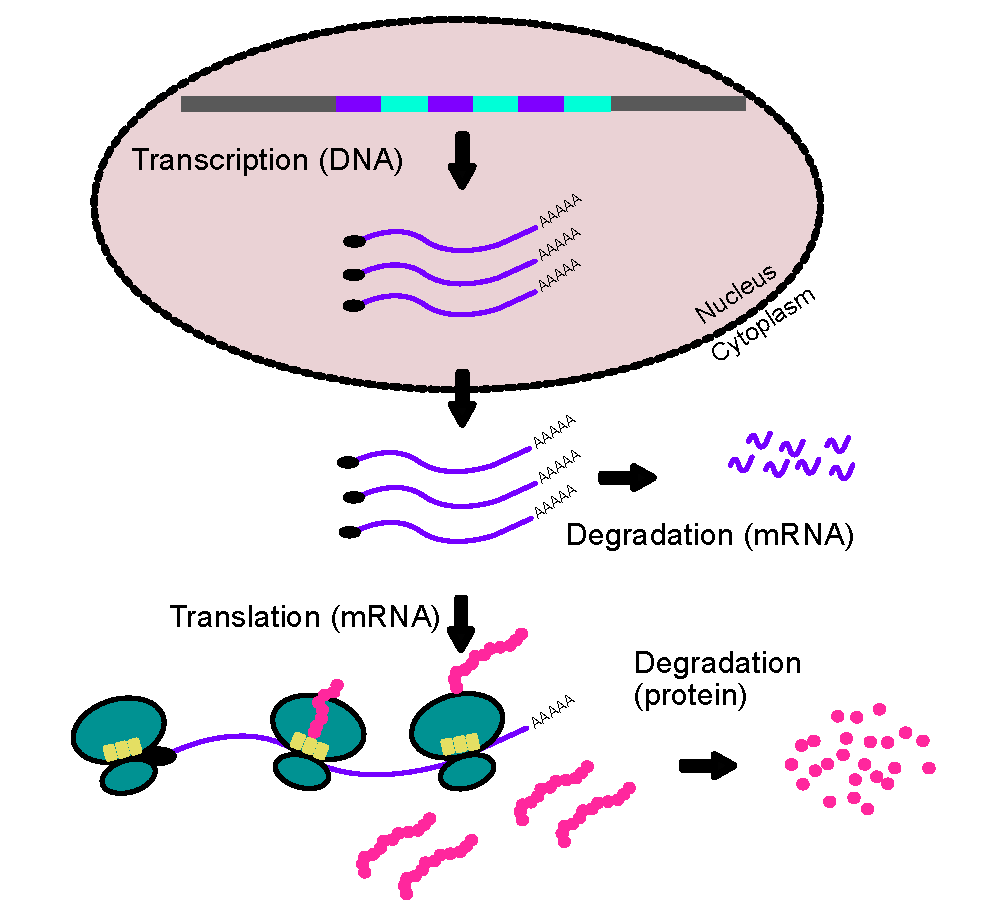
\includegraphics{./figures/geneExprPath_2.pdf}
  \caption{The gene expression pathway - DNA is transcribed into RNA containing a 5' cap (black oval) introns (teal boxes),exons (purple boxes) and a poly(A) tail. RNAs are processed into mRNAs that consisting of a 5' cap, exons and a poly(A) tail. mRNAs can be transported out of the cellular nucleus into the cytoplasm where they can be degraded, stored or translated into proteins depending on cellular demands. Synthesised proteins can be degraded by proteosomes. \label{fig:geneExprPath}}
\end{wrapfigure}

The whole genetic code of an organisms is stored as deoxyribonucleic acid (DNA) molecules in a double stranded formation as highly condensed chromosomes. Transcription is the process whereby temporary copies of the DNA are generated, called transcripts or ribonucleic acid (RNA), and occurs in the cell's core (nucleus). RNAs can undergo processing by which multiple different variants coming from the same region are produced. A subset of processed RNAs is the so called messenger RNA (mRNA). These mRNAs are transported from the nucleus into the cytoplasm where they can be stored, degraded or associate with ribosomes. Ribosomes translate mRNAs in proteins that fulfill major functions within the cell. Proteins themselves can also undergo degradation. (\textbf{see figure \ref{fig:geneExprPath}}). This flow of genetic information into expressed proteins is commonly referred to as the central dogma in molecular biology (F. Crick, 1970).
\clearpage

\subsection{Contribution to gene expression}

Proteins are the last product of the gene expression pathway and carry out the vast majority of all cellular functions. While it is apparent that modulation of protein levels will offer information on the changes in gene expression, it cannot completely answer the question as to why the levels change. In a disease context, protein levels alone might offer sufficient insight to explain phenotypic differences. However, information on how these differences arise mechanistically is obscured. Yet, these differences in underlying biological mechanisms can be used as targets in therapeutic strategies.

Experimental methods to measure gene expression at different steps are often referred to as ``omics'' (e.g.~proteomics for protein expression, transcriptomics for mRNA expression). These methods provide snapshots of the step under scrutiny in a specific context (steady state or perturbation) for a large portion of genes or proteins. Initially, transcriptomics studies approached gene expression with the assumption that mRNA expression is the main determinant for protein levels and therefore could be used as a proxy for them. However, this view was challenged by several landmark studies that observed a poor mRNA to protein correlation and indicated a larger role of post transcriptional regulation in gene expression than previously assumed (de Sousa Abreu, Penalva, Marcotte, \& Vogel, 2009; Lu, Tomfohr, \& Kepler, 2005; Schwanhäusser et al., 2011; Silva \& Vogel, 2016; Vogel \& Marcotte, 2012).

The debate regarding which step of the gene expression pathway contributes most is ongoing, nevertheless an understanding has been reached that the cellular context is a major determinant. At steady state, mRNA levels seem to explain protein abundance best, however in perturbed systems the contribution of transcript abundance alone is not sufficient to explain protein abundance (Liu, Beyer, \& Aebersold, 2016). For example in a study that challenged immune cells, protein levels were dependent on cellular transcript levels (Jovanovic et al., 2015). In contrast a study investigating cells under stress observed extensive modulation at the protein levels, whereas mRNA transcript abundance was only mildly affected (Cheng et al., 2016).

While the contribution of different steps of the gene expression is dependent on many different factors, e.g.~cellular state or treatments, mRNA translation (synthesis of proteins) is an essential process of this pathway. Furthermore, dysregulation of mRNA translation has been observed in multiple diseases, ranging from neurological disorders to cancer which warrants for a comprehensive understanding of this process (Graff et al., 2009; Kapur \& Ackerman, 2018; L. J. Lee et al., 2021; Ruggero, 2013). This thesis will focus on the role of mRNA translation in the context of cancer.
\newline

\section{mRNA translation}
\subsection{Overview of an mRNA}

After transcription, primary RNA transcripts are processed into mRNAs. mRNAs contain a protein coding region which is flanked by untranslated regions (5' and 3' UTRs) that exert translational control over the mRNA (see \ref{regmRNA}). The 5' has a cap that is important for translation initiation (Grifo, Tahara, Morgan, Shatkin, \& Merrick, 1983), while the 3' end has a poly-A tail protecting the mRNA against degradation (Wilusz, Wormington, \& Peltz, 2001). Multiple different mRNAs (isoforms or transcript variants) from the same genomic region exist. These variants can arise due to a process called alternative splicing which alters the exon composition (e.g.~coding region) of an mRNA. These variants can co-exist at the same time and have distinct properties and can perform distinct functions (Joly Anne-Laure et al., 2018). Furthermore, splicing resulting in alternative UTRs for the same mRNA can introduce to differences in translation (Floor \& Doudna, 2016; Jewer et al., 2020).

\begin{wrapfigure}{o}{1\textwidth}
  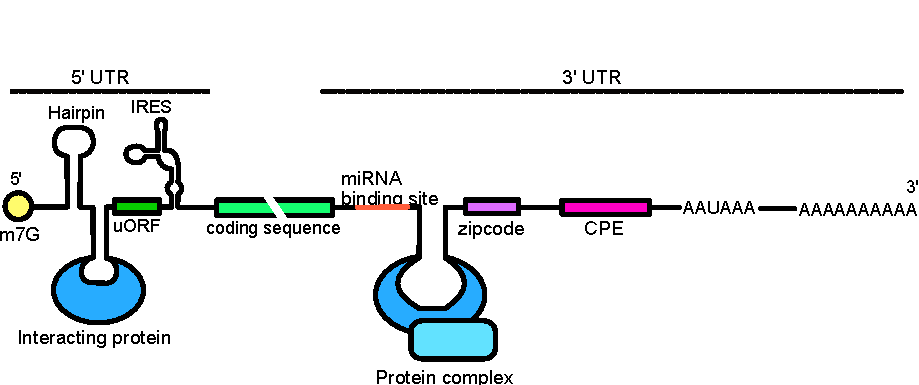
\includegraphics{./figures/UTRFeatures.pdf}
  \caption{ An mRNA consists of a coding sequence (green), 5' (light orange) and 3' (purple) untranslated regions flanking the coding sequence, a 5' cap and a poly-A tail. Located within the 5' and 3' untranslated region are cis elements (light red boxes) that can exert translational control by interfering with ribosomal movement along the mRNA or interact with trans factors (blue and red) or recruit the 43s ribsome (dark green) to the mRNA (see section \ref{regmRNA}). The codon composition of the coding sequence influences translation elongation rates (see section \ref{tRNA}).   
 \label{fig:UTRFeat}}
\end{wrapfigure}
\clearpage
\subsection{Translation of an mRNA}

For the vast majority of protein coding mRNAs, eukaryotic mRNA translation occurs in the cytoplasm, however a small subset of mRNAs is translated in the mitochondria (D'Souza \& Minczuk, 2018). mRNA translation is a process that includes initiation, elongation, termination and ribosome recycling and is an essential process \textbf{see Figure \ref{fig:doodlemRNASteps}}. During the initiation phase a ribosome will associate with the mRNA and starts scanning along the mRNA for a start codon to begin synthesis of the polypeptide chain by incorporating amino acids (Alan G. Hinnebusch, 2014). Amino acids are transferred to the ribosome by specialised RNAs called transfer RNAs (tRNA) that can recognise the genetic code in the mRNA. The availability of tRNAs as well as their modification can influence the rate of elongation. The order by which amino acids are incorporated is dictated by the order of the codons of the open reading frame (ORF). There are more possible codon combinations in comparison to amino acids. This allows that amino acids are encoded by multiple codons, for example lysine is encoded by AAA and AAG. Once the ribosome encounters a stop codon, translation will terminate and the polypeptide chain will be released. The ribosome then disassociates from the mRNA and can be recycled to engage translation of the same or another mRNA. The following sections describe these processes in more detail.

\begin{wrapfigure}{o}{1\textwidth}
  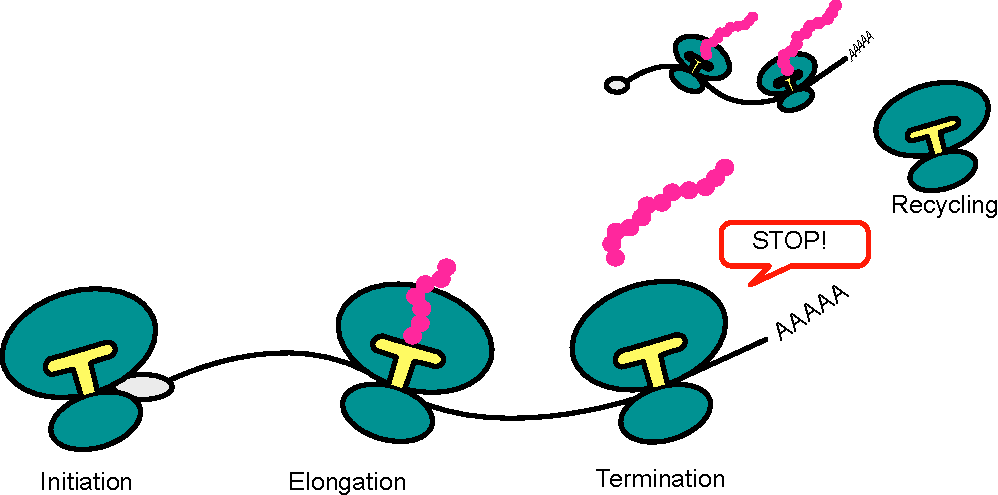
\includegraphics{./figures/doodleTranslation.pdf}
  \caption{mRNA translation initiation, elongation, termination and ribosome recycling steps - The ribosome binds to the mRNA and initiates scanning for a start codon. The elongation phase incorporates amino acids into a polypeptide chain (i.e. the protein product). Once the end of the coding sequence is detected, by recognition of stop codons, the ribosome terminates translation and releases the polypeptide chain. The ribosome can then be recycled to participate in the translation of another mRNA or reinitiate. \label{fig:doodlemRNASteps}}
\end{wrapfigure}
\clearpage

\subsection{Initiation} \label{initiation}

For the initiation to commence, in eukaryotes, two complexes are required; the pre-initiation complex (PIC) and the eukaryotic initiation factor 4F (eIF4F) complex. Both these complexes are governed by signalling pathways that regulate their availability dependent on cellular cues (\textbf{see section \ref{regmRNA}}). The PIC consists of the methionyl-initiatior transfer RNA (met-tRNAi) in a ternary complex (TC) with guanosine triphosphate (GTP) bound eIF2 (Asano, Clayton, Shalev, \& Hinnebusch, 2000). eIF4F is the translation initation complex containing three eIFs: eIF4E, the 5' cap binding protein, eIF4G a scaffold protein and eIF4A and RNA helicase (Grifo, Tahara, Morgan, Shatkin, \& Merrick, 1983; Alan G. Hinnebusch, 2006). eIF4F recruites the PIC to the 5' cap of the mRNA after which scanning for a start codon (AUG) occurs. After AUG recognition eIF2-GTP is hydrolyzed forming a stable 48S PIC. After release of eIF2-GTP the 60S ribosomal subunit joins to form the 80S ribosome and protein synthesis can start (\textbf{Figure \ref{initiation}}).

\subsection{Elongation}

The 80S ribosome contains three sites important for decoding an mRNA: the acceptor (A), peptidyl (P) and exit (E) sites. During elongation in eukaryotes, aminoacytelated tRNAs are delivered to the A-site in a ternary complex with eukaryotic elongation factor 1A (eEF1A) and Guanosine triphosphate (GTP). When the tRNA recognises its cognate codon and pairs, a bond between the amino acid and the polypeptide chain is formed. The formation of the bonds causes the ribosomal units to rotate in relation to each other (Moazed \& Noller, 1989; Munro, Altman, O'Connor, \& Blanchard, 2007). The rotation causes a shift of the tRNA acceptor end from the A and P to the P and E sites, whereas the codon end remains in the A and P site. This is the ``hyrbid'' state of the tRNAs in the ribosome(Dorner, Brunelle, Sharma, \& Green, 2006). eEF2 then promotes the translocation by which the codon end of the tRNA follow into the P and E sites. The deacytelated tRNA is then released from the ribosome. This process is repeated until a stop codon (UAA, UGA or UAG) enters the A site of the ribosome (Hellen, 2018).

\begin{figure}[ht]
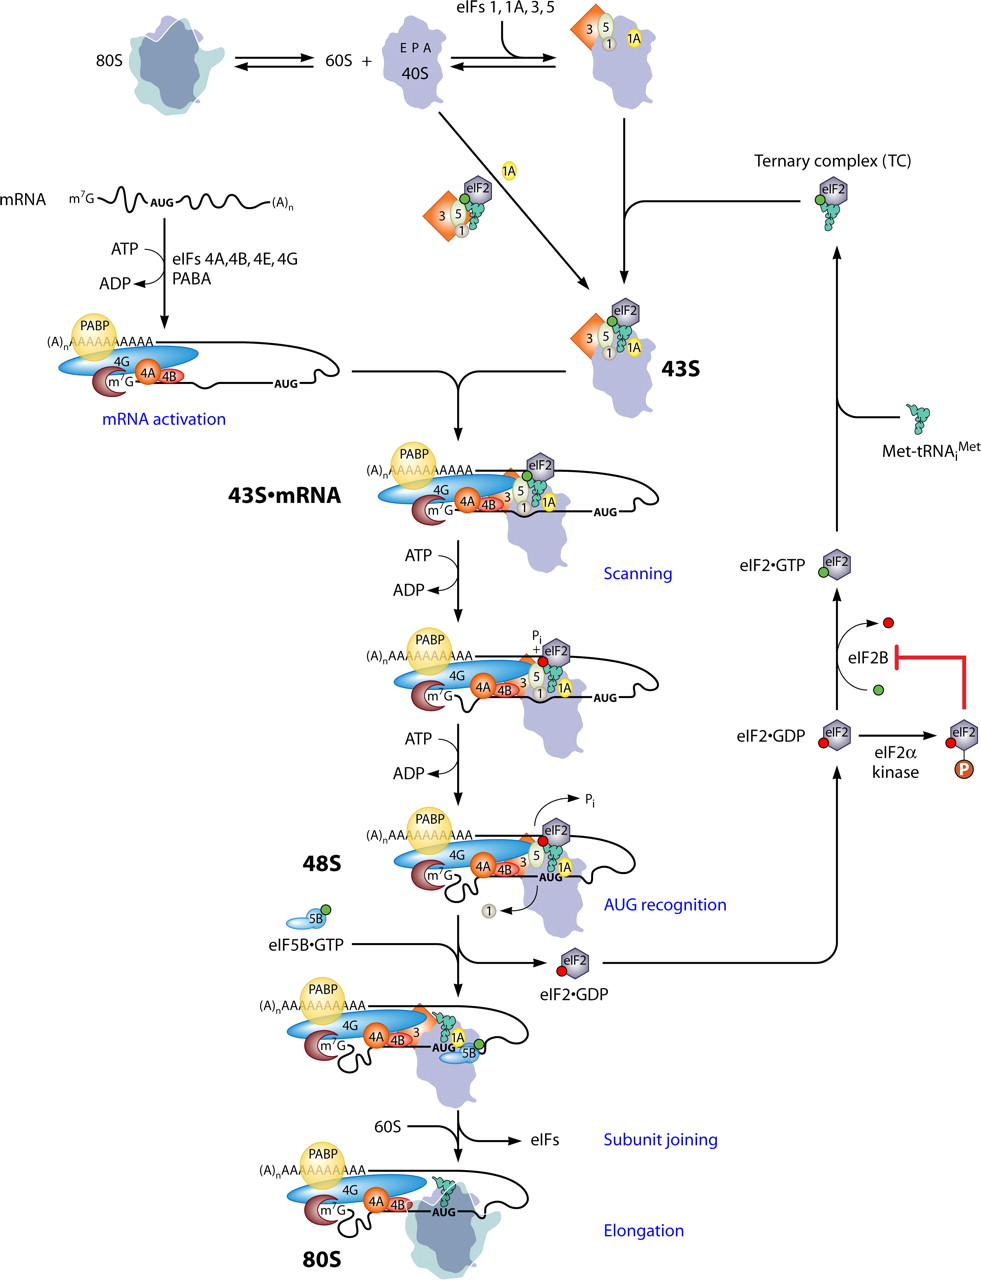
\includegraphics{./figures/initiation.jpg} 
  \caption{Pathway of eukaryotic translation initiation via ribosomal scanning.
  \label{fig:initiation}}
\end{figure}

\clearpage

\subsection{Termination and recycling} 
\begin{wrapfigure}{r}{.4\textwidth}
  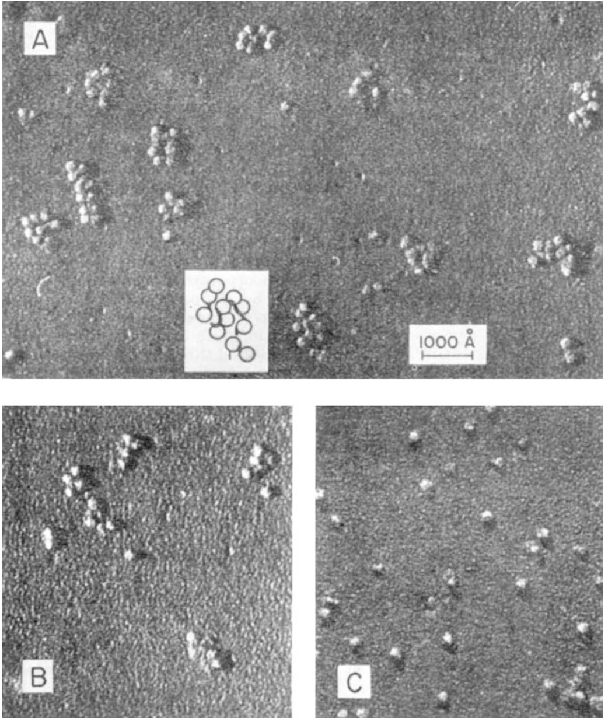
\includegraphics{./figures/polysome.pdf}
  \caption{Electromicrongraph of ribosomes extracted from different positions along a sucrose gradient used for polysome fractionation (A-C). For details on polysome fractionation see section \ref{exptMethod}. Reprinted with permission. DR. T. STAEHELIN et. al. Nature.1963 Aug 31;199:865-70.doi: 10.1038/199865a0. Copyright © 1963, Nature Publishing Group.
  Schematic of the TAPES method - A ribosome (A) can initiate with rate \(\alpha\) on an mRNA with a coding sequence with codons i= 1 ... L. The elongation rate at a specific codon is defined by \(\omega_i\) and \(\beta\) determines the termination rate once a stop codon is encountered. TASEP has been constantly modified, e.g. to allow for correction of initiation or elongation when the following codon is already occupied. Reprinted with permission. Juraj Szavits-Nossan and Martin R. Evans. 10.1103/PhysRevE.101.062404. ©2020 American Physical Society. 
 \label{fig:polysomes}}
\end{wrapfigure}

mRNA translation termination is facilitated by two eukaryotic release factors (eRF), eRF2 and eRF3-GTP (Alkalaeva, Pisarev, Frolova, Kisselev, \& Pestova, 2006; Stansfield et al., 1995). A TC containing eRF2 and eRF3-GTP binds to the A-site of the ribosome upon recognition of a stop codon. This causes an ATP hydrolysis event resulting in a conformational change and release of the polypeptide chain. eRF1 and the ATP binding cassette protein (ABCE1) together promote the splitting of the 60S and 40S subunits after which they can be recycled (Dever \& Green, 2012; Hellen, 2018; Pisarev et al., 2010).

\subsection{Translation efficiency}

Each ribosome synthesises a single protein during translation of an mRNA assuming it is not prematurely terminated. It has been known since the '60s that translation of an mRNA occurs via multiple bound ribosomes (polysomes) simultaneaously (\textbf{see figure \ref{fig:polysomes}A-C}) (Staehelin, Brinton, Wettstein, \& Noll, 1963; Warner, Rich, \& Hall, 1962). Therefore the translation efficiency of an mRNA depends on the number of ribosomes it is associated with. While all steps of translation can affect the translation efficiency of an mRNA, it is most commonly regulated at the initiation step (Dever \& Green, 2012; Jackson, Hellen, \& Pestova, 2010; Richter \& Coller, 2015).

Experimental methods, e.g.~polysome profiling, are used to study translation efficiencies. Furthermore, there are efforts to model translation kinetics such as totally asymmetric simple exclusion process (TASEP) to obtain a better understanding of ribosome movements along the mRNA (MacDonald, Gibbs, \& Pipkin, 1968; Maniloff, 1969) (\textbf{See figure \ref{fig:polysomes}D}). A model that assessed ribosome traffic under steady state and high initiation rates indicates traffic is not only dependent on the densities of ribosomes but also codon specific elongation rates and their distribution along the mRNA (Szavits-Nossan \& Ciandrini, 2020). The next section will go further into detail how initiation rates and elongation can be regulated.
\newline

\section{Regulation of mRNA translation} \label{regmRNA}

mRNA translation is the most energy consuming process in the cell. In rat it was estimated that translation accounts for \textasciitilde20\% of the cellular energy consumption (Buttgereit \& Brand, 1995). The high energy consumption of mRNA translation and its central role in the gene expression pathway requires it to be tightly regulated, especially in cancer where dysregulated metabolism is common (Hanahan \& Weinberg, 2011).

Regulation of translation can be exerted at a global level (i.e.~regulation of a large set of mRNA simultaneously) by e.g.~perturbations of major signalling pathways impinging on mRNA translation. Furthermore, a strong feature of translational control is that it can affect distinct mRNA populations selectively. This form of translational regulation acts on characteristics of mRNAs, e.g.~through cis elements in the UTRs, RNA binding proteins (RBP) or regulation of initiation factors (\textbf{see figure \ref{fig:UTRFeat}}) (Leppek, Das, \& Barna, 2018). Below we will discuss multiple mechanisms that regulate mRNA translation globally or selectively.

\subsection{mTOR} \label{mTOR}

mTOR is a conserved Ser/Thr kinase and is found in two structurally and functionally distinct complexes, mTORC1 and mTORC2 (Pearce et al., 2007; Saxton \& Sabatini, 2017). In a growth promoting environment mTOR switches cell metabolism to increase protein synthesis, lipids and nucleotides, while suppressing catabolic pathways. mTORC2 promotes survival via signalling through protein kinase A (AKT) and is involved in metabolism (Sarbassov, Guertin, Ali, \& Sabatini, 2005).

mTOR activity is modulated via growth factor signalling (i.e.~insulin and insulin-like growth factor; IGF1). Growth factor signalling is mediated through the phosphoinositide 3-kinase (PI3K) / AKT and Ras/mitogen-activated protein kinase (MAPK) pathways. Both these pathways are involved in oncogenic signalling and under investigation as therapeutic targets in cancer (Hilger, Scheulen, \& Strumberg, 2002; Yang et al., 2019). In several cancers (e.g.~breast, lung, prostate and colon) the gene encoding the p110\(\alpha\) subunit of PI3K is frequently mutated or amplified (J. W. Lee et al., 2005; D. A. Levine et al., 2005; Samuels et al., 2004). The E545K mutation leads to a reduced inhibition of p85 at the catalytic p110\(\alpha\) subunit of PI3K (Jiang et al., 2018). In \textbf{study 3} we investigate oncogenic signalling via the PI3K pathway activated by insulin and the role of mTOR in mediating the resulting effects on gene expression in the MCF7 breast cancer cell line that harbours the E545K mutation (Schneck et al., 2013). Furthermore, hyperactivity of PI3K/AKT and Ras/MAPK signalling pathways have been reported in multiple cancers and been linked anti- cancer therapy resistance (Pópulo, Lopes, \& Soares, 2012; Salaroglio, Mungo, Gazzano, Kopecka, \& Riganti, 2019; Tan \& Yu, 2013). mTOR, as a downstream actor of these pathways integrating their signals, has therefore become a focus of anti cancer therapy by either targeting mTORC1 or using dual inhibitors for PI3K and mTOR (Bhat et al., 2015).

\begin{wrapfigure}{r}{0.6\textwidth}
  \includegraphics{./figures/mTORsignal.jpg}
  \caption{Schematic representation of mTOR signaling to the translational machinery. Philippe P. Roux, and Ivan Topisirovic Mol. Cell. Biol. 2018; doi:10.1128/MCB.00070-18. Reprinted with permission. Copyright © 2018, American Society for Microbiology
 \label{fig:mtorsignal}}
\end{wrapfigure}

mTOR also fulfills a central role in metabolic signalling where it integrates amino acid availability, glucose and cellular oxygen levels to form an appropriate response. For example, increased amino acid availability induces relocalisation of mTOR into proximity of Rag GTPases leading to its activation (Sancak et al., 2008). Furthermore, Glucose deprivation and oxygen availability regulate mTOR activity via adenosine-mono-phosphate kinase (AMPK) signalling. AMPK is activated when a shift in the cellular AMP to adenosine-tri-phophate (ATP) ratio is sensed (Kimball, 2006; Sanders, Grondin, Hegarty, Snowden, \& Carling, 2007). While hypoxia (i.e.~deprivation of oxygen) inhibits protein synthesis in normal cells, in breast cancer, protein synthesis was not inhibited during hypoxia which is attributed to uncontrolled mTOR signalling (Connolly, Braunstein, Formenti, \& Schneider, 2006).

Given the central of mTOR governing proliferation, growth and metabolism, which are often deregulated in cancer, it is vital to comprehensively understand mTORC1 signalling herein (Hanahan \& Weinberg, 2011).

\subsubsection{Global regulation of translation via mTOR}

mTOR regulates mRNA translation mainly by regulating availability of eIF4E through phosphorylation of 4E binding proteins (4E-BPs)(Gingras et al., 1999). eIF4E is required for mRNA 5' cap binding and formation of the eIF4F complex. Therefore, inhibition of mTOR leads to a down regulation of cap dependent mRNA translation.
Other downstream targets of mTOR such as S6k has been shown to regulate components of the translation machinery, e.g.~by activation of programmed cell death protein 4(PDCD4). PDCD4 competes for binding to eIF4G with eIF4A (Dorrello et al., 2006; Göke et al., 2002).

\subsubsection{Selective or "mTOR sensitive" regulation of translation}

Selective or ``mTOR sensitive'' regulation of translation acts on transcripts with a terminal oligo pyrimidine motif (TOP mRNAs). This TOP motif consists of a C followed by a stretch of 4-15 pyrimidines directly after the 5' cap. TOP mRNAs show near complete dissociation from ribosomes under conditions when mTOR is inhibited and are enriched for genes encoding for parts of the translation machinery (Meyuhas, 2000; Thoreen et al., 2012; Yamashita et al., 2008). Recent works indicate the importance of La ribonucleoprotein domain family member 1 (LARP1) in regulation of TOP mRNAs with contradictory findings (Fonseca et al., 2015; Hopkins et al., 2016; Jia et al., 2021; Maraia, Mattijssen, Cruz-Gallardo, \& Conte, 2017). A panel of researches were asked to evaluate these findings which led to the establishment of a model for translational regulation via LARP1 (Berman et al., 2021). Herein, LARP1 is thought to bind to the 5' mRNA cap of TOP mRNAs via its DM15 domain and represses translation by obstructing eIF4E binding in instances where mTOR activity is abolished. In environments where mTOR is active phosphorylation of the DM15 occurs by mTOR causing it to release the 5' cap, wile the la domain of LARP1 remains bound to the mRNA thereby stabilizing it to facilitate translation (Berman et al., 2021). Other instances of selective translation are for mRNAs that lack the TOP motif, but show sensitivity to mTOR activity due to its role in eIF4F complex formation.

\subsection{selective regulation through members of the eIF4F complex}

As mentioned before, the eIF4F complex consists of eIF4E, eIF4A and eIF4G and is required for translation of all cap dependent mRNAs. However, characteristics of 5' UTRs introduce variation to how well mRNAs can be translated. Graff et al.~proposed a model of strong and weak mRNAs. Herein, strong mRNAs are widely expressed and represent the majority of cellular mRNAs and are characterised by short unstructured 5' UTRs, e.g.~\(\beta\)-actin. On the other hand, weak mRNAs show long and structured 5' UTRs and encode for potent growth and survival factors, e.g.~c-Myc, ODC1 and VEGF. Translation of ``strong'' mRNAs would remain effective in conditions where eIF4F complex availability would be limited. However, ``weak'' mRNAs show sensitivity eIF4F availability which is dependent on eIF4E expression (Graff, Konicek, Carter, \& Marcusson, 2008). Elevated eIF4E expression is common in cancer and drives malignancy (De Benedetti \& Graff, 2004).

Studies investigated the effects of eIF4A inhibition on mRNA translation and the underlying characteristics of eIF4A dependent mRNAs. Therein, mRNAs that were senstitive to silvesterol treatment showed characteristics of ``weak'' mRNAs, i.e.~long and structured 5' UTRs (Rubio et al., 2014; Waldron, Raza, \& Le Quesne, 2018; Wolfe et al., 2014). In addition one third of eIF4A dependent mRNAs were encoded by genes with multiple 5' UTR variants, while for eIF4A independent mRNAs this was \textless{} 1\% (Rubio et al., 2014). Translation of mRNAs with different 5' UTR variants has recently been implicated to drive cancer cell plasticity towards more ``stem cell like'' phenotypes during hypoxia (Jewer et al., 2020).

Recently, a more nuanced picture for translation of mRNAs sensitive to inhibition of components of the eIF4F complex has been shown (Gandin et al., 2016). Therein, a comparison of treatments with an mTOR inhibitor (i.e.~limiting eIF4F complex assembly) and silvesterol were evaluated leading to identification of mTOR-eIF4E and mTOR-eIF4A senstive mRNAs. Indeed, as shown before mTOR-eIF4A senstive mRNAs were characterised by long and structured 5' UTRs and endoced for pro surival proteins, however their translation was also dependent on eIF4E availability. mTOR-eIF4E sensitive mRNAs were characterised by short 5' UTRs and did not show dependence on eIF4A. Furthermore, these mRNAs encode for proteins related to metabolism.

\subsection{The integrated stress response}

The integrated stress response is a pathway which can be activated through kinases responding to various stress signals. These kinases include Protein kinase R-like endoplasmic reticulum kinase (PERK) which is activated by misfolded peptides in the endoplasmatic reticulum (ER), Heme regulated eIF2alpha kinase (HRI) which is activated during oxidative stress, protein kinase R (PKR) which is activated in response to certain viral infections by binding to double-stranded RNA (dsRNA) and GCN2 which is activated when cells are deprived of amino acids(Dmitry E. Andreev et al., 2015; Guan et al., 2017; Kapur, Monaghan, \& Ackerman, 2017; Lemaire, Lary, \& Cole, 2005; Taniuchi, Miyake, Tsugawa, Oyadomari, \& Oyadomari, 2016). During the integrated stress response the alpha subunit of eIF2 is phosphorylated. Upon eIF2\(\alpha\) phosphorylation, eIF2\(\alpha\) directly engages the guanine nucleotide exchange factor eIF2B and prevents conversion of inactive eIF2-GDP to active eIF2-GTP needed for met-tRNAi incorporation in the TC, therefore inhibiting translation by reducing PIC availability (Sonenberg \& Hinnebusch, 2009) (\textbf{see also figure \ref{fig:initiation}}).

\subsubsection{Global and selective regulation of translation via the ISR}

Global and selective regulation of translation via the ISR is, similar to mTOR signalling, achieved at a global and selective level. Phosphorylation of eIF2 alpha limits ternary complex availability, therefore ribosome recruitment to the 5' cap is limited which results in a reduction of translation initiation. While global translation is reduced upon ISR, translation of a selective subset of mRNA with upstream open reading frames (uORFs) is increased. A uORF is a reading frame that originates in the 5' UTR of an mRNA upstream of which the AUG precedes that of the coding sequence. uORFs can be out of frame with the main ORF (mORF) and, when translated, lower the expression of the mORF (Marilyn Kozak, 1984). ATF4, a transcription factor for stress response genes, contains multiple uORFs of which one partially overlaps with the mORF. Under normal conditions ATF4 mRNA translation is initiated at uORF1 and reinitiation at uORF2 occurs. The overlap of uORF2 with the mORF causes ribosomes to synthesise protein from uORF2 thereby inhibiting the translation of the coding sequence. Limitation of TC availability during ISR causes longer ribosome scanning times leading to that ribosomes scan past uORF2 and initiate at the mORF (Pakos-Zebrucka et al., 2016).

Ribosome profiling studies indicate that 50\% of mammalian mRNAs harbour uORFs. mRNAs containing uORFs include oncogenes and transcripts important in differentiation and cell cycle (Calvo, Pagliarini, \& Mootha, 2009; Ingolia, Lareau, \& Weissman, 2011; Morris, 1995). The surrounding sequence of the uORF is important for initiation of translation. An AUG in the classical Kozak context (i.e.~{[}A,G{]}..\textbf{ATG}G) is most efficient for translation initiation due to better recognition by the ribosome (Calvo, Pagliarini, \& Mootha, 2009; M. Kozak, 1986). However, uORFs that do not contain AUG have been described as well. For example in Fli-1 two conserved uORFs have been described where one contains an AUG and the other GUG (Sarrazin et al., 2000). Translation of either uORF results in different proteins isoforms endoded in the same mRNA. Furthermore, other elements (e.g.~structures) in proximity of the uORF can also influence its translation (Ruan, Hill, Fatemie-Nainie, \& Morris, 1994).

\subsection{Regulation of mRNA translation by tRNAs} \label{tRNA}
\begin{wrapfigure}{o}{0.6\textwidth}
  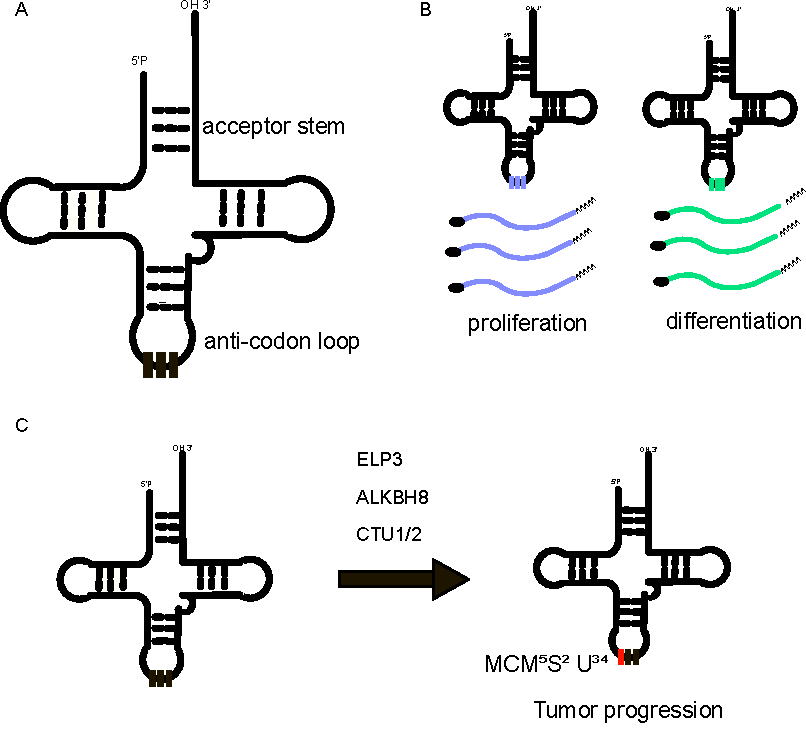
\includegraphics{./figures/tRNA.pdf}
  \caption{ (A) Schematic representation of the tRNA cloverleaf structure with indicated anti-codon and amino acid acceptor sites.  (B) Schematic representation of the proliferation and differentiation mRNAs dependent on distinct tRNA subsets. (C) Schematic representation of the U34 wobble position and the catalytic enzymes involved in this modification that is implied in tumor progression.
 \label{fig:tRNA}}
\end{wrapfigure}

As touched upon earlier, tRNAs are an essential part of the translation machinery that carry the amino acids to the ribosome. tRNAs consist of a 76-90 long nucleotide sequence set into a ``cloverleaf'' structure forming several loops (Sharp, Schaack, Cooley, Burke, \& Soil, 1985) (\textbf{see figure \ref{tRNA}}). The acceptor stem binds the amino acid carried by the tRNA, while the anti-codon loop binds to the mRNA within the ribosome via classical watson-crick pairing (Watson \& Crick, 1953). Multiple codons can encode for the same amino acid (synonymous codons), however the availability of the tRNAs for different codons may vary which can influence elongation rates.

This supply ( i.e.~tRNA availability) and demand (i.e.~codon in expressed mRNA transcripts) relationship has been found to vary across different cellular states, e.g.~proliferation and differentiation. Gingold et. al.~observed two differen tRNA subsets; one induced under proliferation that is otherwise repressed and a subset with similar regulation under differentiation of which the supply matches the codon demand of the transcriptome (Gingold et al., 2014). This model has been disputed and it was proposed that the observed differences would be attributed to GC content in the mRNA (Rudolph et al., 2016). Nevertheless, abbarent tRNA expression and codon usage have been reported in cancer (Z. Zhang et al., 2018). Furthermore, a comprehensive study including small RNAseq (i.e.~for identification of tRNAs) and protein samples across 17 tissues obtained from the The Cancer Genome Atlas (TCGA) reported a tRNA signature stratified by Ki67 (a proliferation marker) staining with implications for patient survival (Hernandez-Alias, Benisty, Schaefer, \& Serrano, 2020). Therefore, while a consensus on proliferation specific tRNA subsets might not have been reached, emerging evidence implicates a role thereof in cancer (Gingold et al., 2014; Hernandez-Alias, Benisty, Schaefer, \& Serrano, 2020; Z. Zhang et al., 2018). More specifically, increased expression of \(tRNA_{CCG}^{Arg}\) and \(tRNA_{UUC}^{Glu}\) has been observed in breast cancer cell lines and proposed to drive metastasis (Goodarzi et al., 2016).

Others report of a role of tRNAs in cancer attributed to tRNA modifications, specifically at the U34 anti- codon (or wobble) position which is highly conserved (El Yacoubi, Bailly, \& de Crécy-Lagard, 2012; Rapino, Delaunay, Zhou, Chariot, \& Close, 2017). Wobbling was proposed by Francis Crick and refers to the ability of non-watson-crick base pairing of tRNA anti codons (F. H. Crick, 1966). This enables a smaller set of tRNAs (41-55 in eukaryotes) to encode for the 64 possible codon combinations (Goodenbour \& Pan, 2006). In mammals, the U34 modification catalytic cascade involves the acetyltransferase Elongator (ELP3), the methyltransferase TRM9-like domain of Alkylation repair homolog 8 (ALKBH8), and the urmylation (URM) pathway, that includes the cytosolic thiouridylase homolog 1 and 2 (CTU1/CTU2) (Kalhor \& Clarke, 2003; Karlsborn et al., 2014). These enzymes ultimately modify the U34 modification into 5-methoxycarbonyl-methyl-2-thiouridine (\(mcm^5s^2U\)) which ensures cognate codon recognition. This modification is thought to occur in a small subset of tRNAs, namely \(tRNA^{UUU}\), \(tRNA^{UUC}\), \(tRNA^{UUG}\), \(tRNA^{UCC}\), and \(tRNA^{UCU}\).

Loss of the ability to modify U34 has been shown to reduce translation elongation rates with varying effects on protein expression (Deng et al., 2015; Nedialkova \& Leidel, 2015; Zinshteyn \& Gilbert, 2013). While in some cases U34 dependent signalling led to ribosome stalling resulting in protein aggregates and increased stress (Nedialkova \& Leidel, 2015; Zinshteyn \& Gilbert, 2013), others reported a subtle dowregulation of proteins encoded by mRNAs requiring U34-modified tRNAs (Deng et al., 2015). U34 modification dependent tRNAs have been shown to play a role in cancer. For example, ELP3 is important in tumor initiation in the intestine and promotes breast cancer invasion as well as progression to metastasis (Delaunay et al., 2016; Ladang et al., 2015). Furthermore, loss of U34 modification in a prostate cancer model lead to an adaptive transcriptional response for mRNAs whose translation was dependent on the U34 modification (Lorent et al., 2019).

\subsection{RNA binding proteins and trans-acting factors}

The UTRs of an mRNA contain sequence elements to which small RNA and RNA binding proteins (RBPs) bind and exert translational regulation. For instance, microRNAs (miRNA), a small class of non coding RNA. The precise role and mechanisms in regulation of translation of miRNAs is still under active investigation (Oliveto, Mancino, Manfrini, \& Biffo, 2017). However, they can directly bind to other RNAs and silence them accomplished through translational repression or destabilisation {[}Jonas2015{]}. Regulation of gene expression by miRNAs has been observed in cancer where miRNAs have been implicated to promote tumorgenesis or act as tumor suppressors (Muniyappa et al., 2009; Nagpal et al., 2015; Sampson et al., 2007; Tian et al., 2010).

RBPs are a class of proteins involved in many regulatory steps of gene expression and account for \textasciitilde7.5\% of the protein coding genes. The poly-A-binding-protein (PABP) is a RBP involved in mRNA translation initiation. PABP is thought to form a closed loop complex of the 3' end to the 5' by interacting with eIF4G. This closed loop is proposed to promote translation and prevent mRNA decay (Afonina, Myasnikov, Shirokov, Klaholz, \& Spirin, 2014; Amrani, Ghosh, Mangus, \& Jacobson, 2008) (\textbf{see also figure \ref{fig:initiation}}). Another important RBP implicated in regulation of translation is Human antigen R (HuR). HuR preferentially binds to AU-rich sequences in the 3' UTR and acts as a stabilizing agent and is involved in RNA-processing (Baou, Norton, \& Murphy, 2011; Fan \& Steitz, 1998; T. D. Levine, Gao, King, Andrews, \& Keene, 1993; Peng, Chen, Xu, \& Shyu, 1998). Furthermore, a study in adenocarcinoma implicates that HuR inhibits translation of proapoptotic factors (Winkler et al., 2014). Other studies in breast, colon and lung cancer observed correlation between HuR and malignancy. Among its targets are HIF-1, VEGF and c-Myc which are known drivers for tumor progression (Denkert et al., 2004; López de Silanes et al., 2003; López de Silanes, Lal, \& Gorospe, 2005).
\newline

\section{Expertimental methods to measure mRNA translation} \label{exptMethod}
\begin{wrapfigure}{r}{0.6\textwidth}
    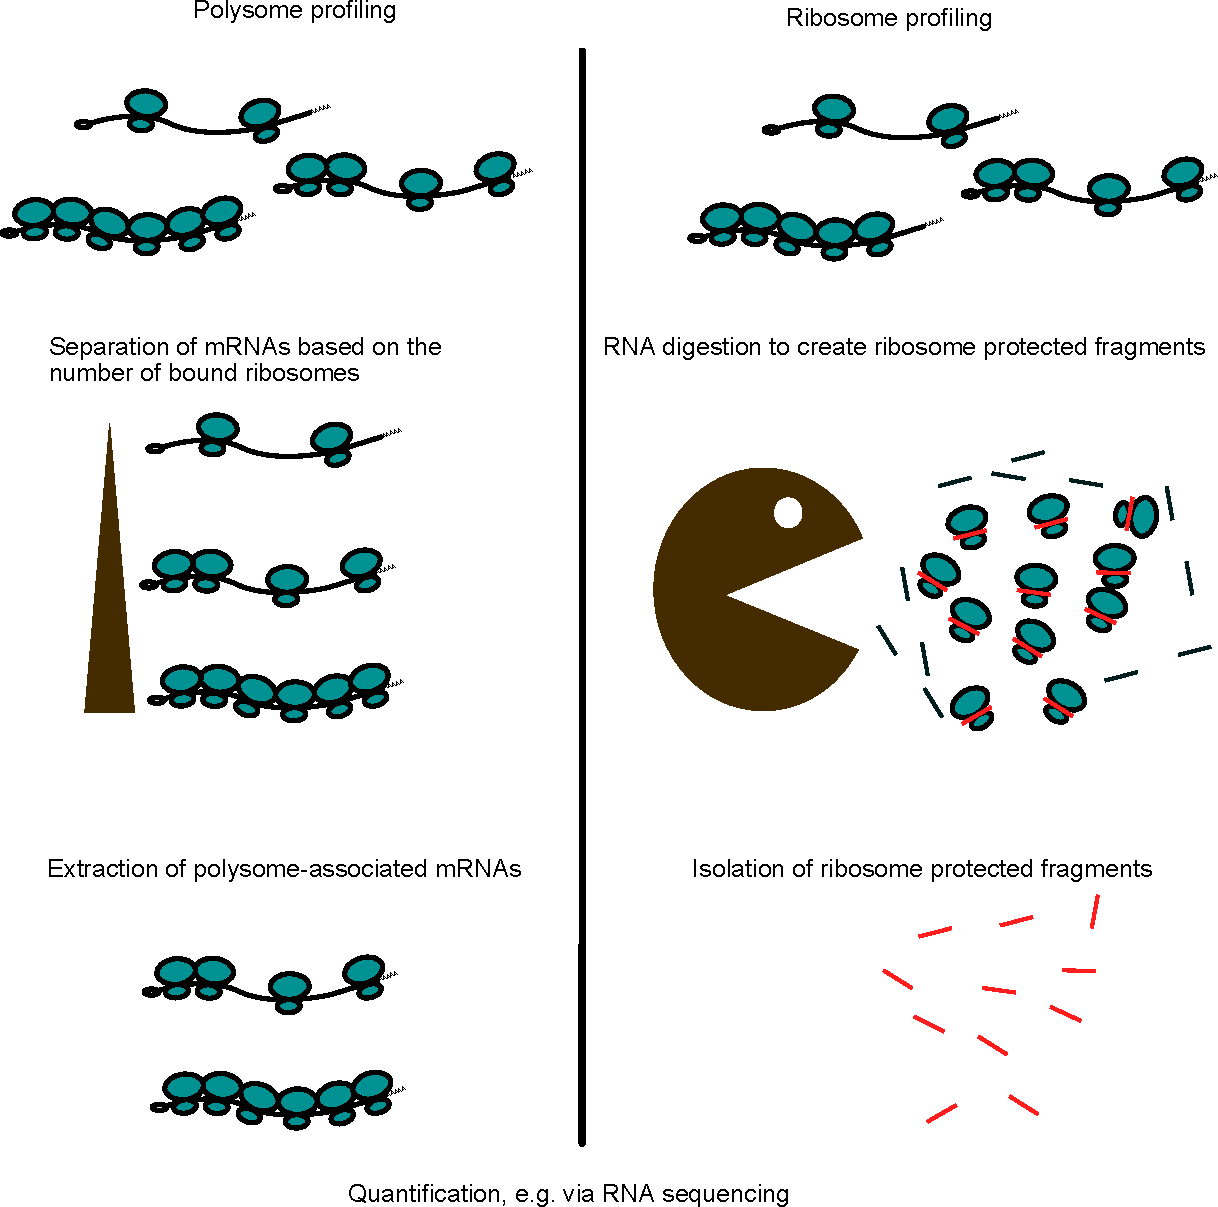
\includegraphics{./figures/polyRibo.pdf}
  \caption{Polysome profiling and ribosome profiling workflows. In polysome profiling a fraction from whole cytoplasmic RNA is loaded onto a sucrose gradient on which they get separated by sedimentation using ultra centrifugation. Fractions corresponding to efficiently translated mRNAs are collected and can be quantified with for example RNA sequencing (left). During ribosome profiling a fraction from the whole cytoplasmic RNA is exposed to a digestion agent which disturbs the RNA. The ribosomes will protect fragments thereby creating ribosome protected fragments. These fragments are then isolated and can be sequenced.  \label{fig:polyRibo}}
\end{wrapfigure}

Methods that measure mRNA translation try to capture the number of ribosomes an mRNA is associated with on the principle that this is directly correlated with their translation efficiency. This is under the assumption that elongation rates across pools of mRNAs are similar which is supported by ribosome kinetic studies (Ingolia, Lareau, \& Weissman, 2011). Two methods are predominantly used for measuring mRNA translation, or changes in translation efficiencies across conditions, namely polysome profiling and ribosome profiling (\textbf{see figure \ref{fig:polyRibo}}). The methods will be explained below in further detail.

\subsection{Polysome profiling}

Polysome profiling is a technique to measure changes in translational efficiencies of mRNAs between two or more conditions. Polysome profiling allows for separation of polysomes from monosomes, ribosomal subunits and messenger ribonucleoprotein particles (mRNPs). During the assay, ribosomes are immobilized on the mRNAs using translation elongation inhibitors (e.g.~cycloheximide). A portion of cytoplasmic RNA extracts then sediment on a linear sucrose gradient (5-50\%) using ultra centrifugation. The resulting gradient is fractionated and mRNAs with different number of bound ribosomes can be extracted and analyzed for changes in translational efficiency (Gandin et al., 2014). Typically fractions belonging to mRNAs with more than 3 bound ribosomes are pooled. A 3-ribosome cut off has been chosen as it is thought to capture most biologically relevant changes in translation efficiency (Gandin et al., 2016).

\begin{wrapfigure}{r}{0.6\textwidth}
    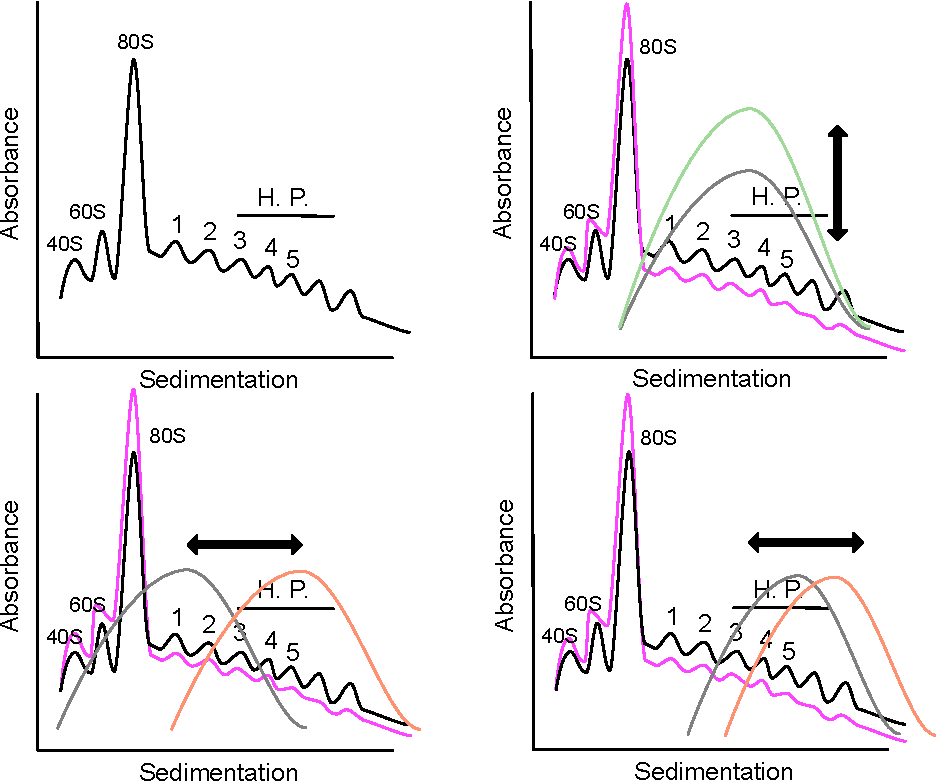
\includegraphics[width=0.9\linewidth]{./figures/polysome_shifts.pdf}
  \caption{Polysome profliles -  (top left) Schematic representation of a polysome profile using linear sucrose gradient fractionation. Indicated in the polysome profiles are the 40S, 60S ribosomal subunits as well as the 80S monosome. H.P. indicates heavy polysome fractions.Between conditions (i.e. black an pink lines) distribution changes for mRNA abundance (grey and green; top right), translation (grey and red; bottom left) and translation within high polysome fractions (grey and red; bottom right) are illustrated. \label{fig:polysome}}
\end{wrapfigure}

An illustration of a polysome profile with peaks for the 40S, 60S subunits and 80S ribosome can be seen in (\textbf{Fig \ref{fig:polysome} top left}). Subsequent peaks along the frations indicate the mRNAs with 2 or more bound ribosomes. mRNAs are typically normally distributed along the fractions, i.e.~in a pool of the same mRNA many will be associated with different numbers of ribosomes (Gandin et al., 2016). Changes in mRNA abundance will lead to an overall increase in the amount of isolated polysome-associated mRNA without a shift of the distribution along the fractions (\textbf{Fig \ref{fig:polysome} top right}). This means that the translation efficiency per mRNA remains unchanged. Changes in translational efficiency can be observed by shifts of polysome association for mRNAs from the light (inefficiently translated) towards the heavy (efficiently translated) polysome fractions or vice versa (\textbf{Fig \ref{fig:polysome} bottom left}). Shift within the heavy polysome fractions (i.e.~with a mean distribution around 4 bound ribosomes to 7 bound ribosomes) can also occur (\textbf{Fig \ref{fig:polysome} bottom right}). Quantification of mRNA levels within each fraction can be assessed using Northern blotting or reverse transcription quantitative polymerase chain reaction (RT-qPCR). For transcriptome wide studies quantification is done using either DNA-microarrays or RNA sequencing.

Pooling of mRNAs as well as collection of multiple fractions makes polysome profiling inconvenient when dealing with large samples sizes or experiments with low amounts of input RNA. Therefore, an optimized sucrose gradient was developed where mRNAs bound to \textgreater3 ribosomes are collected on a sucrose cushion and thereby can be isolated from one single fraction (Liang et al., 2018). This optimized gradient allows for application of polysome profiling in small tissue samples where RNA quantity is limiting and reduces labor intensity of the assay.

Polysome-associated mRNA levels are subject to changes in translation efficiency as well as factors contributing to cytosolic mRNA levels that impact to pool of mRNAs that can associate with ribosomes e.g.~transcription and mRNA stability. Therefore, to identify true changes in translation efficiency it is important to collect cytoplasmic mRNA and polysome-associated mRNA from the same sample in parallel to correct for such mechanisms during downstream analysis.

\subsection{Ribosome profiling} \label{riboseq}

ibosome profiling is a technique that enables sequencing of ribosome protected mRNA fragments (RPFs) (Steitz, 1969). In the assay ribosomes are immobilized on the mRNAs using, similar to polysome profiling, translation elongations inhibitors (e.g.~cyclohexamide (CHX)) (Ingolia, 2016; Ingolia, Ghaemmaghami, Newman, \& Weissman, 2009). One limitation with the use of translation elongation inhibitors is the distortion of ribosome distributions especially at translation initiation sites (Gerashchenko \& Gladyshev, 2014; Hussmann, Patchett, Johnson, Sawyer, \& Press, 2015). For example, treatment with cyclohexamide can affect identification of uORFs in ribosome profiling experiments (Spealman et al., 2018). These introduced artefacts need to be accounted for in the downstream analysis when assessing ribosome position along the mRNA.

RPFs are obtained by RNAse treatment that degrades the links of RNA between ribosomes leaving single ribosomes with a \textasciitilde28 nucleotide long RNA fragment within each ribosome. However, as ribosomal RNAs (rRNA) is also degraded during this process they represent a big fraction herein. The RPFs are then isolated using ultra centrifugation through a sucrose cushion. During this step other RNA fragments such as rRNAs, non-coding RNAs (ncRNAs) or large ribonucleoprotein complexes can co-migrate and contaminate the sample. Typically RPFs with a size ranging from 25-30 nucleotides are selected for quantification. However, among these sizes could be RNA protected by RBPs that have no ribosome associated to it. Furthermore, ribosomes undergoing conformational changes have been shown to protect fragments corresponding to a length of 21nt only when translation elongation is blocked by e.g.~CHX (Lareau, Hite, Hogan, \& Brown, 2014). Therefore, size selection can distort the estimation of translation efficiency from ribosome profiling data (Dmitry E. Andreev et al., 2017). From the resulting RPFs libraries can be constructed and quantified using RNA sequencing. During library construction additional biases due to enzyme sequence preferences can be introduced that can lead wrong estimations of codon positions within the ribosome (Artieri \& Fraser, 2014a).

Initially, fragmented total mRNA using alkaline hydrolysis of the same size were retrieved in paralell to RPFs. This was achieved by extraction of total mRNA from cell lysate followed by purification via recovery of polyadenylated messages or removal of ribosomal RNA (Brar \& Weissman, 2015; Ingolia, Ghaemmaghami, Newman, \& Weissman, 2009). The random fragmentation of total mRNA has been shown to underlie experimental bias. Therefore, now unfragmented total mRNA is sequenced in parallel.

\subsection{Comparing ribosome and polysome profiling}

Albeit both methods generate count data after quantification with RNA sequencing, there are some key aspects that differ between the techniques. Polysome profiling separates efficiently translated mRNAs from non- efficiently translated mRNAs along a sucrose gradient thereby creating an mRNA based perspective for analysing changes in translational efficiencies. In contrast, ribosome profiling determines translational efficiencies by counting the number of RPFs of both efficiently and non-efficiently translated mRNAs. This can have implications for identifaction of transcript variants. For example If a ribosome would not protect a fragment spanning a variant the information would be lost during ribosome profiling (Floor \& Doudna, 2016). Whereas in polysome profiling the quantification is based on the whole mRNA. This gives polysome profiling the advantage in cases of transcript variants with different 5' UTR lengths.

Changes in translational efficiencies, e.g.~shifts in ribosome association, can be dramatic (i.e.~near complete dissociation of ribosomes from an mRNA) or subtle (shifts from e.g.~2 to 4 ribosomes) and could be due to different properties of the mRNAs (Gandin et al., 2016). When these two changes in translation efficiencies are present in parallel, ribosome profiling is biased towards identification of dramatic shifts and masks the subtle ones, leading to false biological conclusions (Gandin et al., 2016). This has been attrituted to the indirect estimation of translation efficiencies from counting RPFs for ribosome profiling, which is highly dependent on the abundance of mRNAs. In polysome profiling this effect is much less pronounced as changes in translation efficiency are directly estimated from the mRNAs associated with heavy polysomes (Masvidal, Hulea, Furic, Topisirovic, \& Larsson, 2017). Higher sensitivity in detecting changes in translational efficiencies on a global scale makes polysome profiling more suitable for transcriptome-wide studies (Gandin et al., 2016; Masvidal, Hulea, Furic, Topisirovic, \& Larsson, 2017).

An advantage of ribosome profiling is that it provides exact nucleotide positions occupied by ribosomes. This offers information at a single nucleotide level where the ribosome sits. Polysome profiling cannot reveal ribosome locations along the mRNA. The single nucleotide resolution of ribosome profiling is necessary in contexts studying local translation events such as ribosomal frame shifts (Rato, Amirova, Bates, Stansfield, \& Wallace, 2011) or uORF translation (Dmitry E. Andreev et al., 2015).

Both methods have their strengths and weaknesses and therefore each method should be considered depending on the underlying biological question.
\newline

\section{Modes for regulation of gene expression through mRNA translation} \label{modes}

From transcriptome-wide assessments of translation using ribosome or polysome profiling expression levels are obtained for both cytoplasmic and polysome-associated mRNAs (or RPFs). For simplicity, from now on, these RNA types will be referred to as total mRNA (i.e.~cytoplasmic mRNA) and translated mRNA (i.e.~polysome-associated mRNA or RPFs). The estimation of expression levels for both translated mRNA and total mRNA allows for interrogation at two steps of the gene expression pathway and their interaction. The interplay of total mRNA with translated mRNA can give valuable insights about the underlying mechanisms that govern gene expression in the studied system.

\begin{wrapfigure}{l}{0.6\textwidth}
  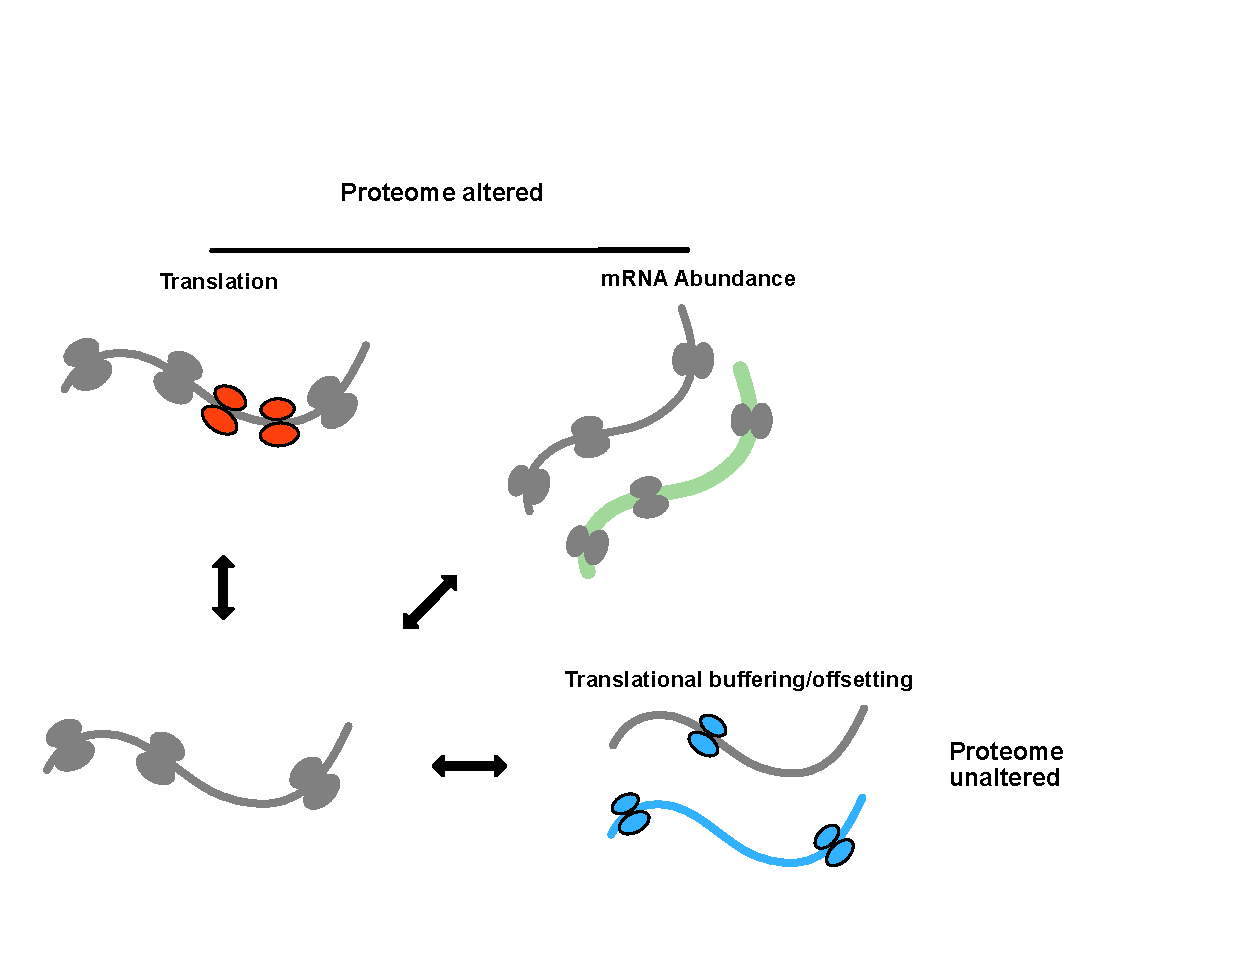
\includegraphics{./figures/geneModes_MRNA.pdf}
  \caption{Regulatory modes of gene expression - Schematic representation of regulatory modes of translation efficiency in a fold-change scatter plot. Indicated in red are changes in translation (i.e. changes in translated mRNA but not total mRNA), in green changes in mRNA abundance (i.e. congruent changes between total mRNA and translated mRNA) and in blue translational buffering (i.e. changes in total mRNA levels but not translated mRNA levels). TE changes as the TE-score would estimate them are indicated.\label{fig:modes}}
\end{wrapfigure}

When comparing perturbed systems to their corresponding control state we typically observe three ``modes'' in which translated mRNA and total mRNA distinctly interact that impact gene expression (\textbf{See figure \ref{modes}}). We refer to these modes as ``translation,'' ``mRNA abundance'' and ``translational buffering.''

\subsection{Translation}

A change in translation occurs when translated mRNA levels either increase or decrease, however corresponding total mRNA levels remain constant or change to a lesser extent resulting in a change of their translation efficiency. A prominent example of this mode can be observed for TOP mRNAs. These mRNAs, under conditions when mTOR is inhibited, show a near complete dissassociation from ribosomes (Gandin et al., 2016). mRNAs under the translation mode are expected to reshape the proteome (\textbf{See figure \ref{modes}}).

\subsection{mRNA Abundance}

Another mode that impacts the proteome is a change in mRNA abundance, here the translated mRNA level changes to a similar magnitude as the total mRNA level. For these mRNAs the translation efficiency is unaltered, as the change in total mRNA levels explains the change in translated mRNA levels. Nevertheless, as there are more (or less) mRNAs being translated an effect the proteome is expected. The underlying biological implication for this mode mRNAs is often related to transcription or mRNA stability (\textbf{See figure \ref{modes}}).

\subsection{Translational buffering} \label{modeBuffering}

The third mode for regulation of gene expression is termed translational buffering. Under this mode a change in total mRNA levels is observed, whereas polysome-associated mRNA levels remain constant between conditions. Translational buffering also reflects a change in translation efficiency as the proportion of mRNAs to associated with ribosomes is altered. In contrast to changes in translation and mRNA abundance, translational buffering has been shown to maintain protein homeostasis rather than reshape the proteome (Lalanne et al., 2018; Lorent et al., 2019; McManus, May, Spealman, \& Shteyman, 2014).

Currently the literature supports multiple forms of translational buffering. Translational buffering can compensate for differences in mRNA levels due to e.g.~differences in gene dosages, so that protein levels remain similar (Dassi et al., 2015; Lalanne et al., 2018). Furthermore, rather than compensating it can ``offset'' translation to temporarily alter the mRNA:protein ratio in response to a stimulus (Lorent et al., 2019).

Translational buffering in its compensation form has been observed at steady state levels. A study comparing co evolution of transcription and translation across seven different organs and mammals showed overall greater divergence of transcription as compared to translation (Wang et al., 2020). Similar compensation at the level of translation has been observed between individuals, tissues and prokaryotes (Artieri \& Fraser, 2014b; Cenik et al., 2015; Dassi et al., 2015; Lalanne et al., 2018; Perl et al., 2017).

Compensation via translational buffering can also enforce equilibration of pathway or protein complex stoichometry (Lalanne et al., 2018; G.-W. Li, Burkhardt, Gross, \& Weissman, 2014). An example of this was observed in evolutionary distant bacetria, i.e.~B. subtilis and E. coli. In B. subtilis translation related factors rpsP and rplS are located in different operons, whereas in E. coli they lie within an operon together with rimM and trmD. While B. subtilis can fine tune transcription at the different operons, in E. coli these will be transcribed together. However, rimM and trmD are only needed in low protein abundance, whereas rpsP and rplS are required in high abundance. E. coli compensates the transcriptional input at the translational level and thus equilibriates for requirements in pathway stoichometry (Lalanne et al., 2018).

As mentioned above a different form of translational buffering can be observed in perturbed systems that offset changes in transcription at the level of translation temporarily. For example, translational offsetting was observed in prostate cancer cells where a transcriptional program was induced under estrogen receptor \(\alpha\) (ER\(\alpha\)) depletion that was showed no increase in polysome-associated mRNA. mRNAs whose transcription was translationally offset required the tRNA u34 modification. ER\(\alpha\) has been shown to regulate the expression of the catalytic enzymes required for the u34 modification (Lorent et al., 2019). Thus, depletion of ER\(\alpha\) led to that tRNAs could not be properly modified at the u34 position and therefore the translation efficiency of mRNAs requiring the modification was reduced despite increased total mRNA levels.
\newline

\section{Algorithms for analysis of changes in translation efficiencies}\label{algorithm}

Given multiple roles of mRNA translation to regulate the proteome via translation, mRNA abundance and buffering it is critical to distinguish them as their underlying mechanisms can have different biological implications. In this section we will discuss methods that analyse polysome-profiling and ribosome profiling data to estimate changes in translation efficiencies across 2 or more conditions and how these methods identify different modes of gene expression.

Initially analysis of transcriptome-wide translation studies used an approach called the translation efficiency (TE-score) that uses the following equation:
\[\varDelta TE = \frac{\frac{P_{c2}}{T_{c2}}} {\frac{P_{c1}}{T_{c1}}}\\\]

This score is calculated the ratio of the ratios between polysome-associated mRNA levels (P) divided by total mRNA levels (T) within each condition (i.e.~C1 and C2). The TE- score approach has been shown to be prone to spurious correlations (Larsson, Sonenberg, \& Nadon, 2010). Spurious correlations arise due to that the ratio of polysome-associated mRNA and total mRNA can systematically correlate with total mRNA levels which is not corrected for in this equation and leads to an elevated type-1 error.

\textbf{Figure \ref{fig:TE}} gives an overview of the relationship between a change in TE-score and each gene expression mode (\textbf{see also figure \ref{fig:modes}}). Changes in mRNA abundance will lead to a \(\varDelta\)TE close to 0 in log space (i.e.~no change in translation efficiency) as total mRNA and translated mRNA change with a similar magnitude. However, in the case of both translation and translational buffering, the nominator and denominator in the TE-score equation change leading to a \(\varDelta\)TE (TE \textless{} 0 or TE \textgreater{} 0) and thereby identification of both changes in translation and translational buffering simultaneously. Therefore, the TE-score method fails to differentiate between changes in translation and translational buffering which can have drastic consequences for the biological interpretation of the results (Oertlin et al., 2019) (\textbf{see also section \ref{modes}}).

\begin{wrapfigure}{o}{0.5\textwidth}
  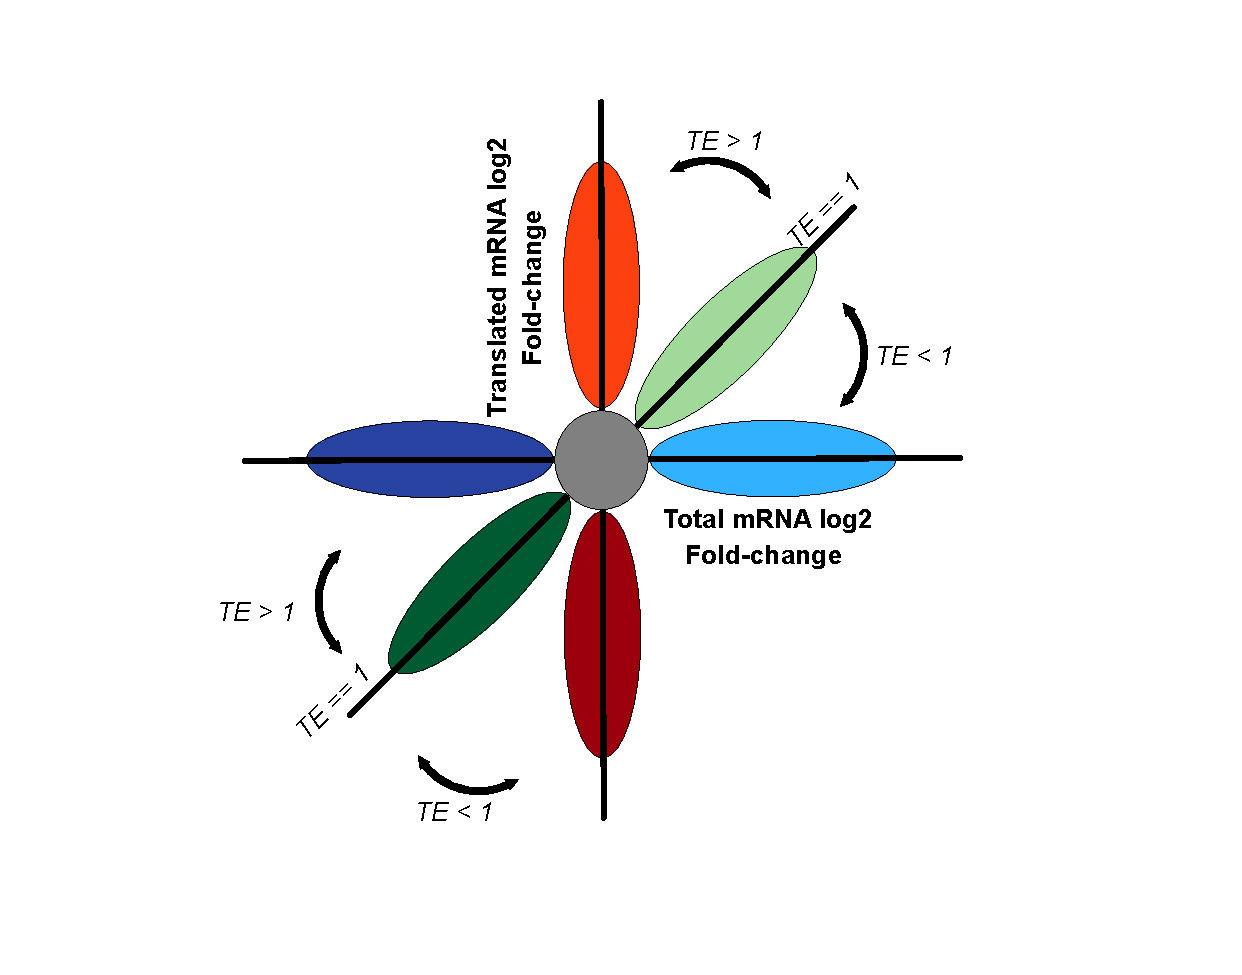
\includegraphics{./figures/geneModes_TE.pdf}
  \caption{TE scores for regulatory modes of gene expression -  Schematic representation of regulatory modes of translation efficiency in a fold-change scatter plot. Indicated in red are changes in translation efficiency altering protein levels, in green changes in mRNA abundance and in blue changes in translation efficiency leading to translational buffering/offsetting. The shifts for the translation efficiency (TE) score are indicated. \label{fig:TE}}
\end{wrapfigure}

The TE-score approach was questioned when proposing the Analysis of Translation Activity (anota) algorithm which was developed for DNA-microarray data (Larsson, Sonenberg, \& Nadon, 2010). anota combines analysis of partial variance (APV) (Schleifer, Eckholdt, Cohen, \& Keller, 1993) with a random variance model (RVM) (Wright \& Simon, 2003). RVM estimates gene variance using shared information across all genes to increase power for detection of differential expression (Wright \& Simon, 2003). anota uses a two-step process that firstly assesses the model assumptions for (i) absence of highly influential data points, (ii) samples classes sharing a common slope, (iii) homoscedasticity of residuals and (iv) normal distribution of per gene residuals. In the second step anota performs analysis of changes in translational activity using the following model:

\[y_{gi} = \beta_g^{RNA}\ X_i^{RNA}+ \beta_g^{cond}\ X_i^{cond} + \varepsilon_{gi}\]

here \(y_{gi}\) is the polysome associated mRNA expression, \(\beta_g^{RNA}\) describes the relationship to total RNA for the \(gth\) gene of the \(ith\) sample column of model matrix \(X\); \(\beta_g^{cond}\) represent the difference in intercept between treatment classes and \(\varepsilon_{gi}\) denotes the residual error.

\begin{wrapfigure}{o}{0.5\textwidth}
  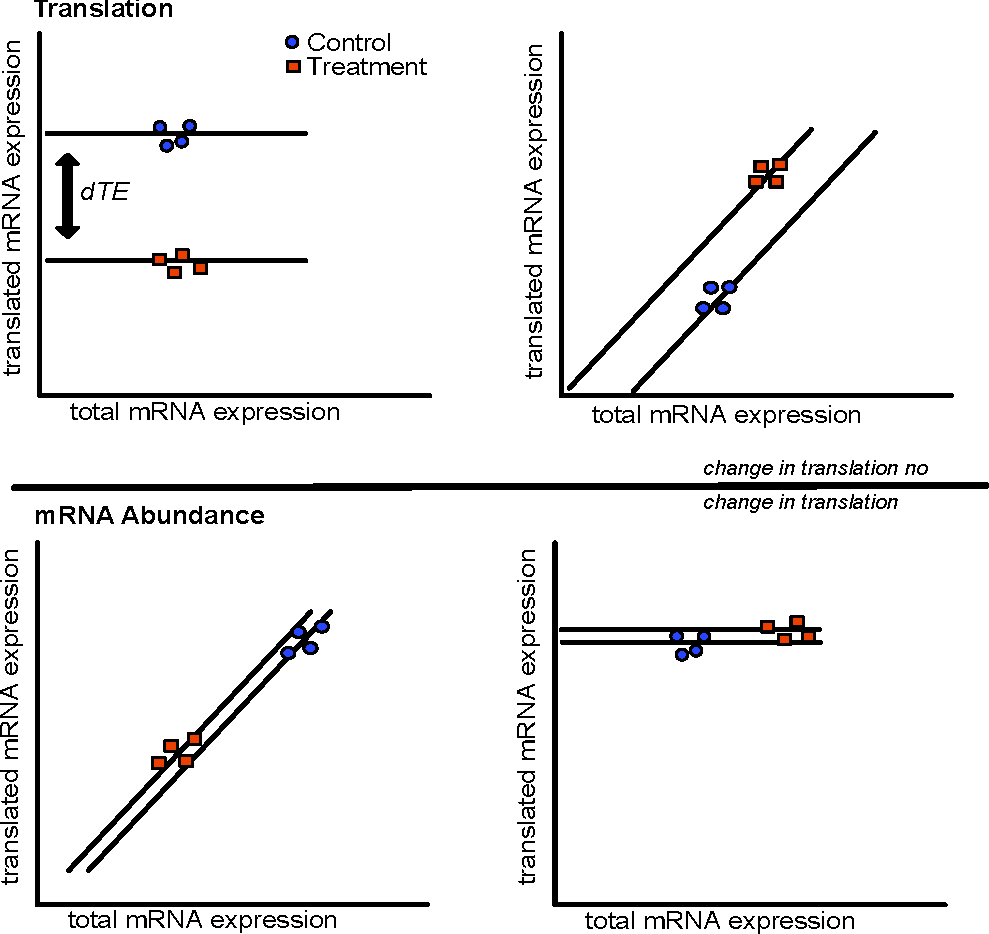
\includegraphics{./figures/geneModes_anota_Larsson.pdf}
  \caption{anota gene models - Schematic representation of the anota analysis models. Translation mRNA expression is set out against total mRNA expression for each biological replicate and treatment condition. Top left shows the model of a gene that is deferentially translated (i.e. change in translated but not total mRNA). The difference in the slope intercepts are used to estimate changes in translation efficiencies between conditions i.e. dTE. Other gene models are shown; change in translation efficiency with varying total mRNA levels (top right); change in mRNA abundance (bottom left) and translational buffering (bottom right).
  \label{fig:anota}}
\end{wrapfigure}

Within anota a common slope for the treatment classes that describes the translated mRNA to total mRNA relationship is calculated. The difference between the slope intercepts is then interpreted as the change in translation efficiency. A simplified view of this model can be seen in (\textbf{Figure \ref{fig:anota} top left}). Here expression for translated mRNA and total mRNA are modeled over two sample classes with each 4 replicates. Furthermore, changes in translation efficiencies can also be observed when translated mRNAs shift to a larger extent than the total mRNA levels (\textbf{Figure \ref{fig:anota} top right}). Identification of genes in this category can be a challenge, especially in highyl variable data set, as they resemble mRNA abundance genes (\textbf{Figure \ref{fig:anota} bottom left}). Nevertheless, using the linear regression analysis anota accurately corrects changes in translated mRNA as can be seen in (\textbf{Figure \ref{fig:anota} bottom right}) where a change in total mRNA but not translated mRNA levels is observed. For this gene the difference in slope intercepts between sample classes is small and will not be identified as differentially translated as would be the case in the TE-score approach. anota was developed at a time where translational buffering was not considered in data sets. Naturally, the methods lacks a setting to analyse translational buffering. This was addressed in anota's successor, anota2seq, and will be discussed in \textbf{Study 1}.

Advances in experimental methods warrant for appropriate statistical methods to analyse data resulting from them. DNA-microarray was the dominant platform to assess transcriptome-wide changes before the advent of RNA sequencing. DNA-microarrays measure intensity after hybridisation events is an indicator of expression, whereas in RNA sequencing reads of constructed libraries are counted. Intensity data from DNA-microarray can be normalised and transformed (i.e.~log transformation) to fulfill the requirements for application of linear models, whereas RNA sequencing harbours additional characteristics that need to be accounted for. Therefore, algorithms developed for analysis of DNA- microarray are not directly applicable to RNA sequencing data as is the case for the anota algorithm.

RNA sequencing data shows variance that is greater than the mean which is commonly referred to as overdispersion. Count data from RNA sequencing have been initially approached using Poisson distributions which assumes that the variance is equal to the mean (Lu, Tomfohr, \& Kepler, 2005). Now established RNA sequencing analysis frameworks such as edgeR and DESeq2 use negative binomial distributions in combination with generalized linear models (GLMs) (Love, Huber, \& Anders, 2014; Robinson, McCarthy, \& Smyth, 2010). The negative binomial distribution uses a dispersion parameter to account for differences in the mean-variance relationship across the expression range (McCarthy, Chen, \& Smyth, 2012). While analysis principles of DESeq2 and edgeR are similar they differ in their normalisation method, dispersion estimation and information sharing across genes. In a simple differential expression analysis between two conditions with one RNA type the GLM model would be as in the following equation:

\[log(y_{gi}) = \beta_g^{cond}\ X_i^{cond} + \varepsilon_{gi}\]

here \(\beta_g^{cond}\ X_i^{cond}\) represent the condition (i.e.~control and treatment) log2 fold change for the \(gth\) gene \(ith\) sample column of the model matrix X and \(\varepsilon_{gi}\) denotes the residual error. When analysing changes in translation effiencies additional parameter for RNA type (i.e.~total mRNA or translated mRNA) and the interaction between the RNA type and condition are added so that:

\[log(y_{gi}) = \beta_g^{RNA}\ X_i^{RNA}+ \beta_g^{cond}\ X_i^{cond} + \beta_g^{RNA:cond}\ X_i^{interaction} + \varepsilon_gi\]

In this model the interaction term is interpreted as the change in translation effiencies (Chothani et al., 2019). Other methods (i.e.~Ribodiff (Zhong et al., 2017), Riborex (W. Li, Wang, Uren, Penalva, \& Smith, 2017) and deltaTE (Chothani et al., 2019)) borrow this analysis principle of an GLM with an interaction term by applying this exact model. A notable difference is that Ribodiff allows dispersion estimation for translated mRNA and total mRNA separately as variance differences between the RNA types can be expected due to varying experimental protocols (Liang et al., 2018; Zhong et al., 2017). While the flexibility of GLMs allows for complex study designs involving 2 or more treatment conditions, Riborex and Ribodiff limit the study design to only two conditions. DeltaTE gives their users full flexibility of the DESeq2 GLM model. Xtail is a method developed for ribosome profiling that makes use of DESeq2 for RNAseq count normalisation (Z. Xiao, Zou, Liu, \& Yang, 2016). Their assessment of differences in translation efficiencies relies on probability matrices for the ratio of translated mRNA over total mRNA within condition and a between condition ratio of these ratios. Babel was the first algorithm designed solely for analysis of differential translation and uses an error-in-variables regression analysis (Olshen et al., 2013). The error-in- variables regression allows accounting for variable total mRNA levels when assessing changes in translation. Although these methods have distinct approaches to identify changes in translation efficiencies, their principle of analysis is similar to comparing a ratio of ratios (see TE-score equation above). Therefore these methods suffer from similar issues as the TE-score which will be discussed in \textbf{Study 1}.

\chapter{Aims of this thesis}

The aims of this thesis are to expand current methodologies for analysis of translation efficiency data and explore the regulation of gene expression in cancer.

In \textbf{Study I} we adapted the ANalysis Of Translation Activity data (anota) algorithm so that it could be applied to next generation sequencing data. Furthermore, we implemented the analysis of translational buffering a recently described regulatory mode of gene expression. The resulting algorithm was named anota2seq.

We then applied the anota2seq algorithm to investigate changes in translation efficiencies in two cancer models:

In \textbf{Study II} we unraveled the effects of eIF4A, an RNA helicase, inhibition using a synthetic rocaglate CR-1-31-B (CR-31) in pancreatic ductal adenocarcinoma.

In \textbf{Study III} we explored the effects of insulin on gene expression in multiple cell lines.

\chapter{Results and discussion}

\section{Study 1 - Generally applicable transcriptome-wide analysis of translation using anota2seq}

Initially changes in translation efficiencies were estimated using the TE-score approach as outlined in section \ref{algorithm}. However, this method was being shown to be prone to spurious correlations leading to elevated false positive identification that can result in false biological conclusions (Larsson, Sonenberg, \& Nadon, 2010). Spurious correlations, when using the TE-score, can be attributed the inadequate correction for changes in total mRNA levels when estimating translation efficiencies (Larsson, Sonenberg, \& Nadon, 2010, 2011). The Analysis of Translation Activity (anota) algorithm facilitates analysis of translational efficiencies that are corrected for changes in total mRNA levels (Larsson, Sonenberg, \& Nadon, 2011).

anota was developed for analysis of transcriptome-wide analysis for data quantified by DNA- microarrays (Larsson, Sonenberg, \& Nadon, 2010). However, advances in experimental methodologies lead to the development in RNA sequencing. RNA sequencing and DNA microarray data have distinct characteristics that need to be accounted for before analysis (\textbf{see section \ref{algorithm}}). Therefore, while the statistical framework of anota had been shown as an adequate approach for analysis of translational efficiencies for data from DNA microarrays it was not directly applicable to RNA sequencing data. The characteristic of RNA sequencing data, that makes applying anota directly not possible, is the mean variance relationship. This encompasses that the counts for lower expressed genes show higher variability than counts for higher expressed genes even after log transformation. Efforts have been made to make RNA sequencing data more ``DNA- microarray like'' so that algorithms developed for intensity based microarray data can be applied to count based RNA sequencing data (Law, Chen, Shi, \& Smyth, 2014; Love, Huber, \& Anders, 2014). Anota2seq, the algorithm developed in this study, allows for transformation and normalisation of RNA sequencing data so that the anota statistical frame work can be applied for analysis of count data.

Another feature of anota2seq is that it allows for statistical analysis of translational buffering. The need for the analysis of translational buffering, or the uncoupling of transcription from translation, has been noted before anota2seq's development by comparing 20 translatomes and transcriptomes with different underlying stimuli in mammalian cells (Tebaldi et al., 2012). The same authors proposed a framework, called tRanslatome, that combines several methodologies for analysis of differential transcription and translation efficiencies, including anota, for a comprehensive analysis of transcription and translation as well as their underlying mechanisms (Tebaldi, Dassi, Kostoska, Viero, \& Quattrone, 2014).

\begin{wrapfigure}{o}{0.5\textwidth}
  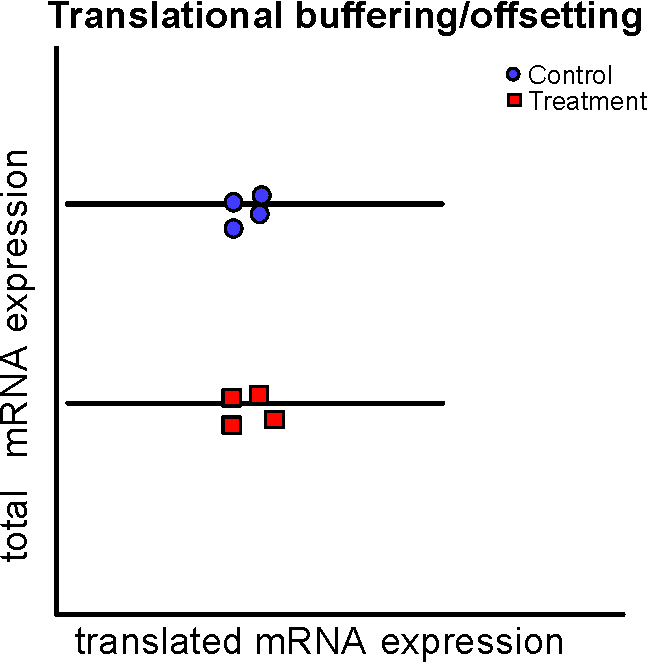
\includegraphics{./figures/geneModes_anota2seq.pdf}
  \caption{anota2seq gene model for analysis of translational buffering /offsetting - Total mRNA expression is set out against translated mRNA expression for each biological replicate and treatment condition. The model shows total mRNA changes that are independent of translated mRNA changes which is classified as translational buffering. It is important to distinguish between the gene modes as their regulation could be due to different underlying biological mechanisms (see section \ref{modes}).
  \label{fig:anota2seq}}
\end{wrapfigure}

Nevertheless, commonly observed in polysome and ribosome profiling data sets are three gene expression modes, translation, translational buffering and mRNA abundance. While anota can be used to identify genes among the translation and mRNA abundance mode, analysis for translational buffering was not implemented therein (\emph{See Figure \ref{fig:anota}}). Therefore, one would need to rely on the integration of several methods to efficiently analyse transcriptome-wide studies of translation efficiences. Anota2seq addresses this issue by changing the analysis model as described in section \ref{algorithm} to analyse changes in total mRNA levels corrected for changes in translated mRNA levels (i.e.~translational buffering, \textbf{see figure \ref{fig:anota2seq}}).

Appliance of anota2seq has successfully identified translational buffering to which biological mechanisms could be linked, e.g.~as mentioned earlier translationally bufferring under ER\(\alpha\) depletion in prostate cancer (\textbf{see section \ref{modeBuffering}}) (Lorent et al., 2019). Furthermore, in \textbf{study 2} translational buffering can be observed as a compensating mechanisms in ``healthy'' cells upon treatment with an eIF4A inhibitor and in \textbf{study 3} we identify mTOR dependent translational buffering for mRNAs with certain 3' UTR characteristics.

The aim of this study was to compare anota2seq's performance to other established algorithms (i.e.~DESeq2, RiboDiff, babel, TE-score and Xtail) for analysis of translation efficiencies, specifically their ability to distinguish the three prominent modes of gene expression. To achieve this we used simulated data. While it is arguable to what extent conclusion drawn from simulated data can be extended towards empirical data it allows for a controlled environment where true positive changes are known in advance. Furthermore, the mean-variance relationship in the simulated data is based on a real polysome profiling data set to increase confidence that drawn conclusions are also applicable to empirical data (Guan et al., 2017). Furthermore, during testing of our simulation we used an additional data set to estimate parameters from to generate data sets. Using these simulated data to compare the performance of the above mentioned algorithms showed almost identical results.

The simulated data consisted of four replicates for translated mRNA and total mRNA with a ``control'' and a ``treatment'' condition. Furthermore, the data sets contained a combination of the following gene sets:

\emph{``Unchanged''}: For this simulation category we sampled reads from the same NB distribution for both the control and treatment conditions in both the translated and total mRNA. This category represents genes that would be unaffected by e.g.~a stimulus of between cellular states.

\emph{``mRNA abundance''}: For this category the control condition for both the translated mRNA and total mRNA were sampled from the same NB distribution. The NB distribution for \textbf{both translated mRNA and total mRNA} of the treatment condition was altered so that values would be drawn corresponding to a fold change (negative or positive) ranging between 1.5 to 3.0. The directionality of the fold changes (i.e.~up or down regulation) was the same for translated mRNA and total mRNA.

\emph{``translation''}: For this category the control condition for both the translated mRNA and total mRNA were samled from the same NB distribution. The NB distribution for \textbf{translated mRNA only} of the treatment condition was altered so that values would be drawn corresponding to a fold change (negative or positive) ranging between 1.5 to 3.0.

\emph{``buffering''}: For this category the control condition for both the translated mRNA and total mRNA were sampled from the same NB distribution. The NB distribution for \textbf{total mRNA only} of the treatment condition was altered so that values would be drawn corresponding to a fold change (negative or positive) ranging between 1.5 to 3.0.

As a first step we tested whether the methods could properly control for type-1 errors (i.e.~false positive identification). For this we simulated a data set with genes belonging only to the ``unchanged'' category. This revealed that babel, but to an even greater extent Xtail, were unable to control their type-1 error as these methods assigned low p-values and FDRs when no real changes were present. DESeq2 was marginally affected by this also. This indicated a limited applicability of Xtail and babel for statistical analysis of translatomes.

From the comparative analysis of the analysis for changes in translation efficiencies affecting protein levels we concluded that anota2seq outperforms all other methods. This was assessed by comparing the area under the curve from Receiver operating characteristics (ROC) and precision recall curves. The ROC curves showed a, albeit slightly, better performance for detecting changes in translation. However, the precision recall was much higher for anota2seq which can be accredited to that the analysis principle of the other methods is based on identifying changes regardless of whether the change is in the translated mRNA or total mRNA (\emph{as explained in section \ref{algorithm}}). Nevertheless, when comparing the performance using simulated data in the absence of genes belonging to the ``buffering'' category anota2seq still showed superior performance.

Next to the a prior knowledge of the introduced changes in the simulation data, it also allowed us to modify parameters to investigate the robustness of the methods to increased variance, overall sequencing depth and differing sequencing depth between samples. Here, all methods showed robustness against variance and sequencing depth differences between samples as long as a minimum of 5 million counts per sample was reached.

A shortcoming in the simulation study is that we did not assess the effects of systematic batch effects. Batch effects can be introduced e.g.~during experimental design and there are many methods that try to correct for these (Johnson, Li, \& Rabinovic, 2007; Leek, 2014; Y. Zhang, Parmigiani, \& Johnson, 2020). Other ways to correct for batch effects is their inclusion in the analysis model, which can be supplied to the analysis model in DESeq2, edgeR as well as anota2seq. Indeed analysis of a dataset with prominent batch effects showed that batch effects can dampen the efficiency of the anota2seq algorithm to identify changes but can be effectively corrected for in the algorithm.

In this study we developed an analysis algorithm for efficient transcriptome-wide analysis of translation efficiencies applicable to DNA-microarrays and RNA seq. Furthermore, anota2seq has been successfully applied to broaden the knowledge around mRNA translation in various different contexts (Chan et al., 2019; Chaparro et al., 2020; Hipolito et al., 2019; Lorent et al., 2019).
\newline

\section{Study 2 - eIF4A supports an oncogenic translation program in pancreatic ductal adenocarcinoma}

Pancreatic cancer is considered a lethal malignancy and has limited treatment options. A study on predictions for european cancer mortality rates for 2021 concluded that health efforts should focus on pancreatic cancer. While other cancers (e.g.~ovary, breast and stomach) showed a decline in mortality rates, no major overall decline was observed for pancreatic cancer in the period of 1970-2021 (Carioli et al., 2021).

Pancreatic ductal adeno carcinoma (PDAC) accounts for over 90\% of exocrine pancreatic cancer, whereas non ductal pancreatic cancers e.g.~acinar cell carcinomas are uncommon (Feldmann, Beaty, Hruban, \& Maitra, 2007; Jun \& Hong, 2016). It is estimated the 60-70\% of the PDACs arise in the head of the pancreas (Luchini, Capelli, \& Scarpa, 2016). So far treatment options are mostly limited to surgical removal, which often is impossible due to the anatomical location of the pancreas head.

With the increasing understanding of tumor heterogeneity, i.e.~tumors with similar tissue origin are diverse at a molecular level, anti cancer therapy improved (Biankin \& Hudson, 2011). In breast cancer stratification by histological, molecular and gene expression features identified several breast cancer subtypes for which different treatment options exist, e.g.~\(ER^+\) breast cancer subtypes respond to endocrine therapy, whereas \(ER^-\) do not (Andre \& Pusztai, 2006; Parker et al., 2009). While breast cancer treatment strategies benefit from a rather well established understanding of the molecular subtypes, in pancreatic cancer transcriptomic based subtyping is still ongoing (Bailey et al., 2016; Collisson et al., 2011; Collisson, Bailey, Chang, \& Biankin, 2019; Moffitt et al., 2015; Puleo et al., 2018). Therefore, it is warranted to extend current knowledge around pancreatic cancer to advance therapeutic strategies in this lethal disease.

While intricacies of molecular subtypes are still being investigated, research has shown that oncogenic mutations in KRAS as well as inactivation of tumor suppressor TP53 are commonly shared among PDAs (Jones et al., 2008). Furthermore, PDAs have been shown to be dependent on increased protein synthesis mediated by KRAS (Chio et al., 2016). This indicates an important role of mRNA translation in PDA.

The aim of \emph{study 2} was to investigate the therapeutic effects of targeting eIF4A in a three dimensional PDA organoid cell culture with mutations in the \(Kras^{LSL-G12D}\), \(Trp53^{LSL-R172H}\) and Pdx1-cre alleles that has been shown to recapitulate PDA tumor progression (Boj et al., 2015). The inhibition of eIF4A was done using a synthetic rocaglate, CR-1-31B (CR-31). Rocaglates have been shown to inhibit eIF4A helicase activity and displayed anti tumor activity (Cencic et al., 2009).

We first wanted to establish the therapeutic validity of targeting eIF4A in PDA. \emph{In vitro} experiments comparing treated PDA organoids (KP) to their normal (N) counter parts revealed heightened sensitivity of KP to CR-31 treatment. OP-puromycin incorporation showed reduced protein synthesis in KP, whereas N were affected to a lesser extent. Furthermore, similar effects were found \emph{in vivo} for PDA tumours. Here CR-31 reduced protein synthesis (assessed by SUnSET assay), tumor growth (assessed by ultra sound imaging) and increased survival. The effect on protein synthesis was not due to inhibition of oncogenic signalling pathways which was evaluated western blot assessing the phosphorylation of e.g.~AKT, mTOR and 4E-BP1. From these findings we concluded that there is therapeutic validity in targeting eIF4A in PDA that acts downstream of oncogenic signalling pathways.

Using polysome profiling we then sought to decipher the mechanisms explaining the increased sensitivity to CR-31 in KP organoids. First we investigated the differences in gene expression between untreated KP and N organoids. Analysis of changes in translation efficiencies using anota2seq revealed massive modulation at both transcription and translation indicative of underlying differences in e.g.~genomic stability and enhanced oncogenic signalling impinging on protein synthesis reported in PDA (Boj et al., 2015). Consistent with the \emph{in vitro} OP-puromycin incorporation and \emph{in vivo} SUNsET experiments, CR-31 had only little effect on translation in N organoids, whereas in KP organoids ample changes in translation were detected.

We then compared the mRNAs affected by CR-31 in KP to the acquired translational profile of untreated KP and N organoids. In order to achieve this we visualised the mRNAs affected by CR-31 in KP onto the data of the untreated KP vs N organoids comparison. This revealed that the acquired translational program of KP organoids is reversed when treated with CR-31.

Performing a similar analysis, we visualised mRNAs sensitive to CR-31 in KP onto the data of the CR-31 treated N organoids. mRNAs affected by CR-31 in KP were translationally offset in CR-31 treated N organoids. Translational buffering, as an adaptive response to treatment, has been shown to maintain protein homeostasis by inducing a transcriptional response increasing the pool of mRNAs that can be translated (Lorent et al., 2019). The ability for N organoids in increase transcription for mRNAs affected by CR-31, whereas KP cannot, could partially explain as to why protein synthesis is not reduced to a similar extent in N as in KP.

We then assessed 5' UTR characteristics of the translationally regulated mRNAs upon CR-31 treatment in KP organoids. It was reported that eIF4A-senstive mRNAs showed overall and more structured 5' UTRs (e.g.~containing G-quadruplexes) (Gandin et al., 2016; Rubio et al., 2014; Wolfe et al., 2014). Furthermore, a mechanisms by which rocaglates would clamp eIF4A to mRNAs with {[}A,G{]} repeats in their 5 UTR was described (Iwasaki, Floor, \& Ingolia, 2016). However, mRNAs sensitive to CR-31 treatment herein showed overall shorter 5' UTRs that were more structured when corrected for their length without enrichment for 4G-quadruplexes or {[}A,G{]} repeats. From the polysome profiling and UTR analysis we concluded that eIF4A supports an oncogenic translation program in PDA cells for mRNAs with shorter but structured 5' UTRs.

Shorter 5' UTRs have been shown to be sensitive to eIF4E expression and encode for metabolic functions (see section \ref{regmRNA}). When we compared an eIF4E overexpression signature in the KP vs N and CR-31 treated KP we observed that in KP organoids translationally regulated mRNAs under eIF4E overexpression were also translationally activated. This observation is consistent with reports of 4E-BP1 loss in pancreatic cancer (Martineau et al., 2014). eIF4A inhibition in tumors resistant to mTOR inhibiton by loss of 4E-BP1 has been shown to circumvent this resistance (Müller et al., 2019). Indeed, CR-31 treatment in KP reversed the translational profile for eIF4E sensitive mRNAs. Therefore, while rocaglates have been shown to directly target eIF4A (Cencic et al., 2009), eIF4F complex formation could be disrupted by reduced eIF4A availability to an extent that also eIF4E dependent translation is affected in PDA organoids herein.

When further inspecting the regulated gene sets in treated and untreated KP compared to their normal counterparts we could see an enrichment in metabolic pathways, e.g.~Oxidative phosphorylation. This pathway was upregulated at the polysome associated RNA levels in untreated KP compared to N, whereas in KP CR-31 treatment reversed the translational profile of this pathway. Indeed, when we measured mitochondrial respiration (by oxygen consumption rates) we found that CR-31 treatment in KP disrupted this process, whereas N organoids where affected to a lesser extent.

A way to counter loss of energy production through oxidative phosphorylation is to increase activity of other anaerobic metabolic pathways, i.e.~glycolysis. However, in CR-31 treated KP we could not detect a upregulation of glycolysis measured by \(U-C^{13}\) glucose labeling and extra cellular acidification rates nor did CR-31 treatment affect expression of glycolytic enzymes (e.g.~HK1,HK2, LDHA, SLCA1, SLCA3). Furthermore, glucose deprivation did not further sensitise to CR-31 treatment. This was rather unexpected, given that increased glycolysis is characteristic for cancers as described by Otto walburg (Warburg, Wind, \& Negelein, 1927). However, the polysome prolfing data revealed translational downregulation and subsequent reduction of protein expression for the glucose transporter Slc2a6. Indeed, perturbation of Slc2a6 using \(sgRNA^{Slc2a6}\) in N and KP organoids revealed a decrease in glucose uptake. From this we concluded that glycolytic compensation of KP is diminished by translational regulation of the glucose transporter Slc2a6 upon CR-31 treatment.

Among the translationally activated genes in the CR-31 treated KP organoids where mRNAs involved in the glutamine metabolism (i.e.~Slc1a5 and Gls1). Furthermore, glutamine levels were elevated in patient derived PDA cell lines treated with CR-31. Glutamine can be converted into \(\alpha\)-ketoglutarate and funneled into the krebs cycle and therefore can serve to increase energy production (Z. Xiao, Zou, Liu, \& Yang, 2016). Indeed, using gas chromatography mass spectrometry (GC/MS) to quantify metabolites after culturing PDA cells in \(C_5^{13}\)- glutamine, we identified a shift towards reductive carboxylation of \(\alpha\)-ketoglutarate obtained from \(C_5^{13}\)- glutamine to produce acetyl-CoA. Notably, the glutamine metabolism was not elevated in N organoids.

A combined treatment of CR-31 with glutaminase inhibitors (BPTES or CB839) could sensitise to CR-31 treatment patient-derived PDA cells to CR-31 treatment. Therefore, our study suggests an eIF4A dependent translational program in PDA that can act as a theurapeutic target in PDA. Furthermore, a recently published ribosome profiling study of a CR-31 treated human pancreatic cancer cell line (PANC1) observed the same therapeutic effect of CR-31 treatment \emph{in vivo} on survival and tumor volume (Singh et al., 2021). This underlines the significance of our study in identifying eIF4A as therapeutic target in PDA.

Nevertheless, the same study indicated differences on the underlying regulated mRNA subsets (Singh et al., 2021). They report, in line with the literature, that eIF4A depdent mRNAs show long and structured 5' UTRs containing \(GGC_4\) sequence motifs they propose to form G-quadruplexes (Singh et al., 2021; Wolfe et al., 2014). While the 5' UTRs of the mRNAs identified herein where overall shorter, they were overall more structured. Also, the mRNAs identifed in Singh et. al.~were involved in KRAS signalling, which was unaltered in our study. Furthermore, Singh et. al.~chose to use ribosome profiling in their study that provides nucleotide resolution of ribosome occupancy (Singh et al., 2021). The nucleotide resolution of ribosome profiling could give insights whether ribosomes stall at G-quadruplex sites. Yet, the authors did not exploit this feature of their applied experimental methodology. Whether G-quadruplexes can actually form stably in cells is still investigated. Waldron et. al.~showed that \(GGC_4\) structures do not form G-quadruplexes, but rather classical hairpin secondary structures and that these dictate eIF4A dependency (Waldron, Raza, \& Le Quesne, 2018).

This raises some questions about the differences between experimental setups and their potential influence on biological outcomes and interpretation thereof. For instance, Singh et. al.~performed ribosome profiling on a PANC1 cell line culture treated with 25nM CR-31, wheres herein we performed polysome profiling on a 3D-organoid culture treated with 10nM CR-31. The differences between ribosome and polysome profiling have been discussed extensively (see section \ref{exptMethod}). Furthermore, by measuring IC50 concentrations for CR-31 in a panel of pancreatic cancer cell lines, Singh et. al.~show a \textasciitilde6-fold difference in susceptability to CR-31 between the cell lines of which PANC1 cells were most sensitive to CR-31. Dosage dependent viability experiments of patient derived PDA cells in our study revealed that at 10nM CR-31 treatment cell viability was reduced by \textasciitilde30\%, whereas treatment with 25nM reduced viability by \textgreater{} 50\%. Furthermore, in patient derived PDA a combination treatment of CR-31 and CB839 showed no synergistic effects at 25nM CR-31, whereas at 12.50nM synergy was observed. Therefore, combining the findings of these two studies indicate that CR-31 treatment in PDA indeed has a therapeutic effect, however the underlying mechanisms that are observed in the transcriptome wide analysis of translation efficiencies could be dependent on the experimental method to assess mRNA translation, the model system and drug concentrations.
\newline

\section{Study 3 - mTOR-dependent translational buffering overrides transcriptome alterations leading to
maintained proteome composition}

Breast cancer is an umbrella term for a heterogeneous disease with numerous molecular subtypes with different clinical behaviour. Currently, breast cancer is classified into five major groups; luminal A, luminal B, HER-2, basal and normal like. The classification is based on histopatholgy and receptor status. Histopathological are determined by the degree of tumor differentiation (tubule formation), nuclear pleomorphism and proliferation (mitotic count). These features are then scored into a histological grade (I-III) (Eliyatkın, Yalçın, Zengel, Aktaş, \& Vardar, 2015). As mentioned earlier, receptor status of the progesterone (PR), estrogen (ER) and HER-2 are evaluated and have implications for neo adjuvant and adjuvant treatment strategies. Advances in technologies lead to classification of breast cancer subtypes using gene expression profiles,e.g.~the PAM50 classification, that allow for unbiased classification of breast cancer (Parker et al., 2009). A study that correlated the gene expression profiles of the PAM50 classification found a significanlty higher mRNA:protein correlation for PAm50 genes, indicating their prognostic value (Johansson et al., 2019). Nevertheless, the authors observed intermixed luminal B and HER2 clustering based on protein expression in line with the literature that HER2 subtypes receive conflicting mRNA based classifications (Johansson et al., 2019; Prat et al., 2014). Thus, the understanding of breast cancer subtypes has increased tremendously leading to improved and targeted treatment options, however there is need for further research to understand the full breast cancer spectrum on a molecular level.

Another important factor to consider in breast cancer treatment are life style and other health related issues that could impact cancer progression or response to treatment, e.g.~obesity. Studies in the 1970 observed unfavorable prognosis for breast cancer in obese women (Abe, Kumagai, Kimura, Hirosaki, \& Nakamura, 1976). More recent studies observed endocrine therapy to be less effective in obese patients and increased cancer incidence in individuals with higher weight or lack of physical activity (Eheman et al., 2012; K. Lee, Kruper, Dieli-Conwright, \& Mortimer, 2019). Obesity can pose an increased risk to develop metabolic disorders such as metabolic syndrome or type 2 diabetes that can lead to hyperinsulinemia, i.e.~elevated physiological insulin levels (Saltiel, 2001).

The role of insulin in the body is to regulate glucose and lipid metabolism as well as protein synthesis. Protein synthesis and metaboloism are often dysregulated in cancer (Hanahan \& Weinberg, 2011; Saltiel, 2001). Insulin can bind to both IGF1R and INSR that activate the PI3K/AKT/mTOR and RAS/ERK signalling pathways. A role of insulin in cancer progression has initially been observed in long term tissues cultures where it increased metabolism as well as growth (Osborne, Bolan, Monaco, \& Lippman, 1976). Another growth factor that is similar to insulin is IGF1 which acts to the same receptors as insulin. IGF1 plays a role in cancer progression and its levels are elevated upon hyperinsulinemia (Bailyes et al., 1997; Christopoulos, Msaouel, \& Koutsilieris, 2015; Gallagher \& LeRoith, 2010; Molinaro et al., 2019).

The importance of both IGF1 and insulin signalling in cancer has been well established now and led to development of therapeutic strategies by e.g.~targeting both IGF1R and INSR or the PI3K signalling pathway (Kuijjer et al., 2013; Mayer et al., 2017). Yet, to this day the full extent of insulin signalling on gene expression in cancer has not been established. This study aims to bridge this gap in knowledge by elucidating the effects of insulin signalling on gene expression using a multi-omics (including transcriptomics, translatomics and proteomics) approach to capture multiple steps of the gene expression pathway simultaneously. Furthermore, we asses insulin signalling in cancer cells as well as non-transformed epithelial cells.

We first investigated the effects of insulin on gene expression in a luminal A breast cancer cell line, i.e.~MCF7 cells. Polysome-profiling revealed a strong transcripional and translational response upon insulin stimulation. Among the translationally activated mRNAs were mRNAs with short 5' UTRs that harboured TOP motifs which is n accordance that insulin signalling leads to activation of mTORC1 and phosphorylation of its downstream targets. When visualising the mRNAs in the data where MCF7 cells were stimulated with insulin in the presence of torin1, an mTOR active site inhibitor, we observed that the changes in mRNA translation were almost fully reversed. This led to the conclusion that the effects of insulin on gene expression are to a great extent dependent on mTOR activity.

What was surprising to us was the observation that a subset of mRNAs exhibited translational buffering upon insulin stimulation while mTOR is inhibited. For these mRNAs, the total mRNA levels were increased, whereas the polysome-association was unaltered between conditions effectively uncoupling transcription from translation. As has been seen by others, we confirm that translationally buffered mRNAs maintain constant protein expression across conditions using HiRIEF LC/MS (Branca et al., 2014; Lorent et al., 2019). These findings indicate that mTOR can act as a gatekeeper for transcriptional programs to fine tune translation in response to extra cellular or intra cellular signals.

MCF7 cells are of epithelial origin and therefore not ``classical'' insulin sensitive such as adipose tissue or muscle cells. Their strong response to insulin prompted us to investigate whether this could be due to cellular plasticity in cancer. To assess this we chose to compare the effects found in MCF7 to a non-malignant epithelial cell type, i.e.~HMEC cells. We found that insulin alone was not sufficient to stimulate the PI3k/AKT/mTOR pathway in HMEC to a similar extent as in MCF7. However, a combination treatment of insulin and IGF1 in HMEC cells elicited a similar reponse as insulin treatment in MCF7 alone. Furthermore, it is known that during hyperinsulinemia IGF1 levels are increased and both IGF1 and insulin signalling has been associated with cancer (Gallagher \& LeRoith, 2010). We therefore opted to compare the combined insulin + IGF1 treatment in HMEC to that of MCF7 assuming their signalling cascades are nearly identical as proposed in the literature (Boucher, Tseng, \& Kahn, 2010; Pollak, 2008).

Polysome profiling of the insulin + IGF1 stimulated HMEC cells revealed a strong translational response, but was lacking the transcriptional activation found in MCF7 cells. Translationally activated mRNAs in HMEC showed 5' UTR features similar to those in MCF7 cells. Consequently, their translational activation was dependent on mTOR signalling evident from their translational suppression under conditions when mTOR was inhibited during insulin + IGF stimulation. Furthermore, comparing the mRNA signatures of HMEC and MCF7 in the opposite cell line we observed that changes at the level of translation were almost fully in accord across cell types.

In contrast to MCF7 cells, HMEC did not elicit a strong transcriptional response as shown by the small number of changes in mRNA abundance. However, when comparing a recently described transcription signature induced after INSR translocation to the nucleus, we could see that in both HMEC and MCF7 these mRNA show changes in total mRNA levels but of differing magnitude (Hancock et al., 2019). A possible explanation for the different response in transcription could be due to differences in chromosome instability between the cell lines that expose different parts of the DNA to trans acting factors. While not assessed herein, a transcription factor analysis paired with chromatin immunoprecipitation (ChIP) sequencing could provide insight into this (Park, 2009; Solomon, Larsen, \& Varshavsky, 1988). Assuming a consequence of having a weaker transcriptional response, HMEC cells did not elicit translational buffering upon insulin + IGF1 stimulation when mTOR was inhibited. Thus the effects of insulin and IGF1 signalling on mRNA translation are foremost mTOR dependent, however total mRNA responses differ between malignant and non-malignant epithelial cells.

The translational buffering in MCF7 prompted us to investigate this phenomenon more. To assess differences dependent on mRNA characteristics we defined two subsets. The ``reversed'' and the ``uncoupled'' (that is translationally buffered when mTOR is inhibited) subsets that only differed in their total mRNA response when mTOR was inhibited during insulin stimulation. To rule out that the observed effects on total mRNA are technical artifacts we validated total mRNA levels for two genes from each subset. The differences in regulation of gene expression were not dependent on codon usage which has been described before in a different context (Lorent et al., 2019). However, overall uncoupled mRNAs had shorter 3' UTRs with a higher GC content and were depleted for HuR binding sites.

The depletion of HuR binding sites in the 3' UTRs of the uncoupled subset prompted us to investigate mRNA stability differences. Using a time series experiment under actinomycin D treatment to block transcription quantified using nanoString, we found significant longer mRNA half lifes for the uncoupled subset as compared to the reversed subset. From these data we hypothesised that there are different underlying mechanisms that regulate gene expression under conditions where mRNA translation is dampened between these subsets. Under this hypothesis the reversed subset is likely regulated through mRNA stability, whereas the more stable uncoupled subset requires to be regulated by translation as their total mRNA level remains high for longer periods of time.

The involvement of HuR in this cannot be fully supported with our current data as the analysis only supports a correlation between the occurrence of HuR binding sites and the 3' UTRs of the reversed subset. The effect on stability could be due to other trans acting factors such as miRNAs (Valinezhad Orang, Safaralizadeh, \& Kazemzadeh-Bavili, 2014). A way to increase confidence is to investigate HuRs involvement experimentally, e.g.~we could use a sgRNA to silence HuR and measure total mRNA levels of the reversed and uncoupled mRNAs previously validated by qPCR. If HuR is involved, we would expect that the reversed mRNAs retain higher total mRNA levels under the condition where mTOR is inhibited during insulin stimulation in MCF7 cells as compared to control. Furthermore, while the differences in total mRNA levels between the insulin and the insulin and torin1 treated conditions in the RNAseq data imply a treatment effect on the mRNA stability we did not observe this in the time chase experiment quantified by nanoString. This raises the question whether the transcription block induced by actinomycin D could influence the regulation of mRNA stability between treatments. We could address this by including actinomycin D in the sgHuR experiment and see if effects thereof differ or an experiment independent of sgHuR. Presence of such an effect could indicate a cross talk between transcription and regulation of mRNA stability.

Since the translational buffering identified herein was only observed in insulin treated cancer cells, we wondered whether this is only specific to this system. Cellular plasticity in cancer allows cancer cells to obtain stem cell like features (Jewer et al., 2020; Quail, Taylor, \& Postovit, 2012; Wahl \& Spike, 2017). Therefore, we reasoned that a system were we study gene expression of stem cells could give some insight whether cancer cells obtained stem cell features that normal epithelial cells do not have. Furthermore, we wanted to investigate whether other means of mTOR inactivation, e.g.~hypoxia, would lead to similar effects on gene expression. To assess these aspects we cultured H9 stem cells in medium with insulin present in normoxia and hypoxia. This experimental setup differs to that of MCF7 and HMEC cells as these were serum starved (i.e.~no insulin in medium) prior to induction with insulin.

Studying this system in H9 we could observe changes for all three modes for regulation of gene expression. Most notably, we observed a large fraction of translationally buffered mRNAs with similar 3' UTR characteristics to that of the uncoupled subset in MCF7 cells. Using publicly available data on mRNA stability we saw that the translationally buffered mRNA were overall more stable as compared to their background. Furthermore, visualising the reversed and uncoupled subset identified in MCF7 in the H9 data we observe differences in their regulation of total mRNA levels, indicating that these subset underlie different modes of regulation even across these two models. Furthermore, these data argue for that translational buffering observed in insulin treated MCF7 cells during mTOR inhibition is not limited to that system but can also occur under more physiological conditions.

Here we present an unprecedented and comprehensive investigation of the effects on insulin on gene expression in cancer cells and non- transformed epithelial cells across multiple steps of the gene expression pathway. Our results indicate that cancer cells have acquired an increased sensitivity to insulin signalling as compared to non-transformed epithelial cells that is largely dependent on mTOR in both cell types. Furthermore, we observed that cancer cells have the ability to translationally buffer mRNAs which is a feature they share with stem cells.

\chapter{Conclusions}

Cancer is a vastly heterogeneous disease that is characterised by uncontrollable growth and proliferation as well as dysregulated metabolism that can evade therapy through acquiring resistance. mRNA translation is a common denominator of these processes and it is therefore paramount to understand the precise mechanisms by which mRNA translation is regulated to better formulate therapeutic strategies against cancer.

This thesis provides an advance in methodology to analyse transcriptome-wide changes translation efficiencies that can be applied to study cancer models. Using this methodology in the context of pancreatic cancer we could propose a possible new therapeutic strategy for this lethal disease where treatment options are limited. Lastly, we explore the effects of insulin on gene expression in an unprecedented study that highlighted an adapted insulin responsiveness of cancer cells. Furthermore, we illuminate the ability of cancer cells to translationally buffer genes which is a feature they share with stem cells and could therefore be an acquired mechanism.

Taken together this thesis provides insight on gene expression in two different cancer models that could potentially lead to clinical applications. While these studies are a step forward, more research is needed to grasp the full extent of the mechanisms involved in cancer.

\hypertarget{acknowledgments}{%
\chapter*{Acknowledgments}\label{acknowledgments}}
\addcontentsline{toc}{chapter}{Acknowledgments}

\hypertarget{references}{%
\chapter*{References}\label{references}}
\addcontentsline{toc}{chapter}{References}

\hypertarget{refs}{}
\begin{CSLReferences}{1}{0}
\leavevmode\hypertarget{ref-Abe1976}{}%
Abe, R., Kumagai, N., Kimura, M., Hirosaki, A., \& Nakamura, T. (1976). Biological characteristics of breast cancer in obesity. \emph{The Tohoku Journal of Experimental Medicine}, \emph{120}(4), 351--359. \url{https://doi.org/10.1620/tjem.120.351}

\leavevmode\hypertarget{ref-Afonina2014}{}%
Afonina, Z. A., Myasnikov, A. G., Shirokov, V. A., Klaholz, B. P., \& Spirin, A. S. (2014). Formation of circular polyribosomes on eukaryotic {mRNA} without cap-structure and poly({A})-tail: A cryo electron tomography study. \emph{Nucleic Acids Research}, \emph{42}(14), 9461--9469. \url{https://doi.org/10.1093/nar/gku599}

\leavevmode\hypertarget{ref-Alkalaeva2006}{}%
Alkalaeva, E. Z., Pisarev, A. V., Frolova, L. Y., Kisselev, L. L., \& Pestova, T. V. (2006). In {Vitro Reconstitution} of {Eukaryotic Translation Reveals Cooperativity} between {Release Factors eRF1} and {eRF3}. \emph{Cell}, \emph{125}(6), 1125--1136. \url{https://doi.org/10.1016/j.cell.2006.04.035}

\leavevmode\hypertarget{ref-Amrani2008}{}%
Amrani, N., Ghosh, S., Mangus, D. A., \& Jacobson, A. (2008). Translation factors promote the formation of two states of the closed-loop {mRNP}. \emph{Nature}, \emph{453}(7199), 1276--1280. \url{https://doi.org/10.1038/nature06974}

\leavevmode\hypertarget{ref-Andre2006}{}%
Andre, F., \& Pusztai, L. (2006). Molecular classification of breast cancer: Implications for selection of adjuvant chemotherapy. \emph{Nature Clinical Practice Oncology}, \emph{3}(11, 11), 621--632. \url{https://doi.org/10.1038/ncponc0636}

\leavevmode\hypertarget{ref-Andreev2017}{}%
Andreev, Dmitry E., O'Connor, P. B. F., Loughran, G., Dmitriev, S. E., Baranov, P. V., \& Shatsky, I. N. (2017). Insights into the mechanisms of eukaryotic translation gained with ribosome profiling. \emph{Nucleic Acids Research}, \emph{45}(2), 513--526. \url{https://doi.org/10.1093/nar/gkw1190}

\leavevmode\hypertarget{ref-Andreev2015}{}%
Andreev, Dmitry E., O'Connor, P. B., Fahey, C., Kenny, E. M., Terenin, I. M., Dmitriev, S. E., \ldots{} Baranov, P. V. (2015). Translation of 5' leaders is pervasive in genes resistant to {eIF2} repression. \emph{eLife}, \emph{4}, e03971. \url{https://doi.org/10.7554/eLife.03971}

\leavevmode\hypertarget{ref-Artieri2014a}{}%
Artieri, C. G., \& Fraser, H. B. (2014a). Accounting for biases in riboprofiling data indicates a major role for proline in stalling translation. \emph{Genome Research}, \emph{24}(12), 2011--2021. \url{https://doi.org/10.1101/gr.175893.114}

\leavevmode\hypertarget{ref-Artieri2014}{}%
Artieri, C. G., \& Fraser, H. B. (2014b). Evolution at two levels of gene expression in yeast. \emph{Genome Research}, \emph{24}(3), 411--421. \url{https://doi.org/10.1101/gr.165522.113}

\leavevmode\hypertarget{ref-Asano2000}{}%
Asano, K., Clayton, J., Shalev, A., \& Hinnebusch, A. G. (2000). A multifactor complex of eukaryotic initiation factors, {eIF1}, {eIF2}, {eIF3}, {eIF5}, and initiator {tRNAMet} is an important translation initiation intermediate in vivo. \emph{Genes \& Development}, \emph{14}(19), 2534--2546. \url{https://doi.org/10.1101/gad.831800}

\leavevmode\hypertarget{ref-Bailey2016}{}%
Bailey, P., Chang, D. K., Nones, K., Johns, A. L., Patch, A.-M., Gingras, M.-C., \ldots{} Grimmond, S. M. (2016). Genomic analyses identify molecular subtypes of pancreatic cancer. \emph{Nature}, \emph{531}(7592), 47--52. \url{https://doi.org/10.1038/nature16965}

\leavevmode\hypertarget{ref-Bailyes1997}{}%
Bailyes, E. M., Navé, B. T., Soos, M. A., Orr, S. R., Hayward, A. C., \& Siddle, K. (1997). Insulin receptor/{IGF}-{I} receptor hybrids are widely distributed in mammalian tissues: Quantification of individual receptor species by selective immunoprecipitation and immunoblotting. \emph{The Biochemical Journal}, \emph{327 ( Pt 1)}, 209--215. \url{https://doi.org/10.1042/bj3270209}

\leavevmode\hypertarget{ref-Baou2011}{}%
Baou, M., Norton, J. D., \& Murphy, J. J. (2011). {AU}-rich {RNA} binding proteins in hematopoiesis and leukemogenesis. \emph{Blood}, \emph{118}(22), 5732--5740. \url{https://doi.org/10.1182/blood-2011-07-347237}

\leavevmode\hypertarget{ref-Berman2021}{}%
Berman, A. J., Thoreen, C. C., Dedeic, Z., Chettle, J., Roux, P. P., \& Blagden, S. P. (2021). Controversies around the function of {LARP1}. \emph{RNA Biology}, \emph{18}(2), 207--217. \url{https://doi.org/10.1080/15476286.2020.1733787}

\leavevmode\hypertarget{ref-Bhat2015}{}%
Bhat, M., Robichaud, N., Hulea, L., Sonenberg, N., Pelletier, J., \& Topisirovic, I. (2015). Targeting the translation machinery in cancer. \emph{Nature Reviews Drug Discovery}, \emph{14}(4, 4), 261--278. \url{https://doi.org/10.1038/nrd4505}

\leavevmode\hypertarget{ref-Biankin2011}{}%
Biankin, A. V., \& Hudson, T. J. (2011). Somatic variation and cancer: Therapies lost in the mix. \emph{Human Genetics}, \emph{130}(1), 79--91. \url{https://doi.org/10.1007/s00439-011-1010-0}

\leavevmode\hypertarget{ref-Boj2015}{}%
Boj, S. F., Hwang, C.-I., Baker, L. A., Chio, I. I. C., Engle, D. D., Corbo, V., \ldots{} Tuveson, D. A. (2015). Organoid {Models} of {Human} and {Mouse Ductal Pancreatic Cancer}. \emph{Cell}, \emph{160}(1), 324--338. \url{https://doi.org/10.1016/j.cell.2014.12.021}

\leavevmode\hypertarget{ref-Boucher2010}{}%
Boucher, J., Tseng, Y.-H., \& Kahn, C. R. (2010). Insulin and insulin-like growth factor-1 receptors act as ligand-specific amplitude modulators of a common pathway regulating gene transcription. \emph{The Journal of Biological Chemistry}, \emph{285}(22), 17235--17245. \url{https://doi.org/10.1074/jbc.M110.118620}

\leavevmode\hypertarget{ref-Branca2014}{}%
Branca, R. M. M., Orre, L. M., Johansson, H. J., Granholm, V., Huss, M., Pérez-Bercoff, Å., \ldots{} Lehtiö, J. (2014). {HiRIEF LC}-{MS} enables deep proteome coverage and unbiased proteogenomics. \emph{Nature Methods}, \emph{11}(1, 1), 59--62. \url{https://doi.org/10.1038/nmeth.2732}

\leavevmode\hypertarget{ref-Brar2015}{}%
Brar, G. A., \& Weissman, J. S. (2015). Ribosome profiling reveals the what, when, where and how of protein synthesis. \emph{Nature Reviews. Molecular Cell Biology}, \emph{16}(11), 651--664. \url{https://doi.org/10.1038/nrm4069}

\leavevmode\hypertarget{ref-Buttgereit1995}{}%
Buttgereit, F., \& Brand, M. D. (1995). A hierarchy of {ATP}-consuming processes in mammalian cells. \emph{The Biochemical Journal}, \emph{312 ( Pt 1)}, 163--7. \url{https://doi.org/10.1042/bj3120163}

\leavevmode\hypertarget{ref-Calvo2009}{}%
Calvo, S. E., Pagliarini, D. J., \& Mootha, V. K. (2009). Upstream open reading frames cause widespread reduction of protein expression and are polymorphic among humans. \emph{Proceedings of the National Academy of Sciences}, \emph{106}(18), 7507--7512. \url{https://doi.org/10.1073/pnas.0810916106}

\leavevmode\hypertarget{ref-Carioli2021}{}%
Carioli, G., Malvezzi, M., Bertuccio, P., Boffetta, P., Levi, F., Vecchia, C. L., \& Negri, E. (2021). European cancer mortality predictions for the year 2021 with focus on pancreatic and female lung cancer. \emph{Annals of Oncology}, \emph{0}(0). \url{https://doi.org/10.1016/j.annonc.2021.01.006}

\leavevmode\hypertarget{ref-Cencic2009}{}%
Cencic, R., Carrier, M., Galicia-Vázquez, G., Bordeleau, M.-E., Sukarieh, R., Bourdeau, A., \ldots{} Pelletier, J. (2009). Antitumor {Activity} and {Mechanism} of {Action} of the {Cyclopenta}{[}b{]}benzofuran, {Silvestrol}. \emph{PLoS ONE}, \emph{4}(4). \url{https://doi.org/10.1371/journal.pone.0005223}

\leavevmode\hypertarget{ref-Cenik2015}{}%
Cenik, C., Cenik, E. S., Byeon, G. W., Grubert, F., Candille, S. I., Spacek, D., \ldots{} Snyder, M. P. (2015). Integrative analysis of {RNA}, translation, and protein levels reveals distinct regulatory variation across humans. \emph{Genome Research}, \emph{25}(11), 1610--1621. \url{https://doi.org/10.1101/gr.193342.115}

\leavevmode\hypertarget{ref-Chan2019}{}%
Chan, K., Robert, F., Oertlin, C., Kapeller-Libermann, D., Avizonis, D., Gutierrez, J., \ldots{} Chio, I. I. C. (2019). {eIF4A} supports an oncogenic translation program in pancreatic ductal adenocarcinoma. \emph{Nature Communications}, \emph{10}(1, 1), 5151. \url{https://doi.org/10.1038/s41467-019-13086-5}

\leavevmode\hypertarget{ref-Chaparro2020}{}%
Chaparro, V., Leroux, L.-P., Masvidal, L., Lorent, J., Graber, T. E., Zimmermann, A., \ldots{} Jaramillo, M. (2020). Translational profiling of macrophages infected with {Leishmania} donovani identifies {mTOR}- and {eIF4A}-sensitive immune-related transcripts. \emph{PLOS Pathogens}, \emph{16}(6), e1008291. \url{https://doi.org/10.1371/journal.ppat.1008291}

\leavevmode\hypertarget{ref-Cheng2016}{}%
Cheng, Z., Teo, G., Krueger, S., Rock, T. M., Koh, H. W. L., Choi, H., \& Vogel, C. (2016). Differential dynamics of the mammalian {mRNA} and protein expression response to misfolding stress. \emph{Molecular Systems Biology}, \emph{12}(1), 855. \url{https://doi.org/10.15252/msb.20156423}

\leavevmode\hypertarget{ref-Chio2016}{}%
Chio, I. I. C., Jafarnejad, S. M., Ponz-Sarvise, M., Park, Y., Rivera, K., Palm, W., \ldots{} Tuveson, D. A. (2016). {NRF2 Promotes Tumor Maintenance} by {Modulating mRNA Translation} in {Pancreatic Cancer}. \emph{Cell}, \emph{166}(4), 963--976. \url{https://doi.org/10.1016/j.cell.2016.06.056}

\leavevmode\hypertarget{ref-Chothani2019}{}%
Chothani, S., Adami, E., Ouyang, J. F., Viswanathan, S., Hubner, N., Cook, S. A., \ldots{} Rackham, O. J. L. (2019). {deltaTE}: {Detection} of {Translationally Regulated Genes} by {Integrative Analysis} of {Ribo}-seq and {RNA}-seq {Data}. \emph{Current Protocols in Molecular Biology}, \emph{129}(1), e108. \url{https://doi.org/10.1002/cpmb.108}

\leavevmode\hypertarget{ref-Christopoulos2015}{}%
Christopoulos, P. F., Msaouel, P., \& Koutsilieris, M. (2015). The role of the insulin-like growth factor-1 system in breast cancer. \emph{Molecular Cancer}, \emph{14}(1), 43. \url{https://doi.org/10.1186/s12943-015-0291-7}

\leavevmode\hypertarget{ref-Collisson2019}{}%
Collisson, E. A., Bailey, P., Chang, D. K., \& Biankin, A. V. (2019). Molecular subtypes of pancreatic cancer. \emph{Nature Reviews Gastroenterology \& Hepatology}, \emph{16}(4, 4), 207--220. \url{https://doi.org/10.1038/s41575-019-0109-y}

\leavevmode\hypertarget{ref-Collisson2011}{}%
Collisson, E. A., Sadanandam, A., Olson, P., Gibb, W. J., Truitt, M., Gu, S., \ldots{} Gray, J. W. (2011). Subtypes of pancreatic ductal adenocarcinoma and their differing responses to therapy. \emph{Nature Medicine}, \emph{17}(4), 500--503. \url{https://doi.org/10.1038/nm.2344}

\leavevmode\hypertarget{ref-Connolly2006}{}%
Connolly, E., Braunstein, S., Formenti, S., \& Schneider, R. J. (2006). Hypoxia inhibits protein synthesis through a {4E}-{BP1} and elongation factor 2 kinase pathway controlled by {mTOR} and uncoupled in breast cancer cells. \emph{Molecular and Cellular Biology}, \emph{26}(10), 3955--3965. \url{https://doi.org/10.1128/MCB.26.10.3955-3965.2006}

\leavevmode\hypertarget{ref-Crick1970}{}%
Crick, F. (1970). Central {Dogma} of {Molecular Biology}. \emph{Nature}, \emph{227}(5258, 5258), 561--563. \url{https://doi.org/10.1038/227561a0}

\leavevmode\hypertarget{ref-Crick1966}{}%
Crick, F. H. (1966). Codon--anticodon pairing: The wobble hypothesis. \emph{Journal of Molecular Biology}, \emph{19}(2), 548--555. \url{https://doi.org/10.1016/s0022-2836(66)80022-0}

\leavevmode\hypertarget{ref-DSouza2018}{}%
D'Souza, A. R., \& Minczuk, M. (2018). Mitochondrial transcription and translation: overview. \emph{Essays in Biochemistry}, \emph{62}(3), 309--320. \url{https://doi.org/10.1042/EBC20170102}

\leavevmode\hypertarget{ref-Dassi2015}{}%
Dassi, E., Greco, V., Sidarovich, V., Zuccotti, P., Arseni, N., Scaruffi, P., \ldots{} Quattrone, A. (2015). Translational compensation of genomic instability in neuroblastoma. \emph{Scientific Reports}, \emph{5}(1, 1), 14364. \url{https://doi.org/10.1038/srep14364}

\leavevmode\hypertarget{ref-DeBenedetti2004}{}%
De Benedetti, A., \& Graff, J. R. (2004). {eIF}-{4E} expression and its role in malignancies and metastases. \emph{Oncogene}, \emph{23}(18), 3189--3199. \url{https://doi.org/10.1038/sj.onc.1207545}

\leavevmode\hypertarget{ref-deSousaAbreu2009}{}%
de Sousa Abreu, R., Penalva, L. O., Marcotte, E. M., \& Vogel, C. (2009). Global signatures of protein and {mRNA} expression levels. \emph{Molecular bioSystems}, \emph{5}(12), 1512--1526. \url{https://doi.org/10.1039/b908315d}

\leavevmode\hypertarget{ref-Delaunay2016}{}%
Delaunay, S., Rapino, F., Tharun, L., Zhou, Z., Heukamp, L., Termathe, M., \ldots{} Close, P. (2016). Elp3 links {tRNA} modification to {IRES}-dependent translation of {LEF1} to sustain metastasis in breast cancer. \emph{Journal of Experimental Medicine}, \emph{213}(11), 2503--2523. \url{https://doi.org/10.1084/jem.20160397}

\leavevmode\hypertarget{ref-Deng2015}{}%
Deng, W., Babu, I. R., Su, D., Yin, S., Begley, T. J., \& Dedon, P. C. (2015). Trm9-{Catalyzed tRNA Modifications Regulate Global Protein Expression} by {Codon}-{Biased Translation}. \emph{PLOS Genetics}, \emph{11}(12), e1005706. \url{https://doi.org/10.1371/journal.pgen.1005706}

\leavevmode\hypertarget{ref-Denkert2004}{}%
Denkert, C., Weichert, W., Winzer, K.-J., Müller, B.-M., Noske, A., Niesporek, S., \ldots{} Hauptmann, S. (2004). Expression of the {ELAV}-{Like Protein HuR Is Associated} with {Higher Tumor Grade} and {Increased Cyclooxygenase}-2 {Expression} in {Human Breast Carcinoma}. \emph{Clinical Cancer Research}, \emph{10}(16), 5580--5586. \url{https://doi.org/10.1158/1078-0432.CCR-04-0070}

\leavevmode\hypertarget{ref-Dever2012}{}%
Dever, T. E., \& Green, R. (2012). The elongation, termination, and recycling phases of translation in eukaryotes. \emph{Cold Spring Harbor Perspectives in Biology}, \emph{4}(7), 1--16. \url{https://doi.org/10.1101/cshperspect.a013706}

\leavevmode\hypertarget{ref-Dorner2006}{}%
Dorner, S., Brunelle, J. L., Sharma, D., \& Green, R. (2006). The hybrid state of {tRNA} binding is an authentic translation elongation intermediate. \emph{Nature Structural \& Molecular Biology}, \emph{13}(3), 234--241. \url{https://doi.org/10.1038/nsmb1060}

\leavevmode\hypertarget{ref-Dorrello2006}{}%
Dorrello, N. V., Peschiaroli, A., Guardavaccaro, D., Colburn, N. H., Sherman, N. E., \& Pagano, M. (2006). {S6K1}- and {ßTRCP}p{Mediated Degradation}n of{PDCD4 Promotes Protein Translation}n and{Cell Growth}. \emph{Science}, \emph{314}(5798), 467--471. \url{https://doi.org/10.1126/science.1130276}

\leavevmode\hypertarget{ref-Eheman2012}{}%
Eheman, C., Henley, S. J., Ballard-Barbash, R., Jacobs, E. J., Schymura, M. J., Noone, A.-M., \ldots{} Edwards, B. K. (2012). Annual {Report} to the {Nation} on the status of cancer, 1975-2008, featuring cancers associated with excess weight and lack of sufficient physical activity. \emph{Cancer}, \emph{118}(9), 2338--2366. \url{https://doi.org/10.1002/cncr.27514}

\leavevmode\hypertarget{ref-ElYacoubi2012}{}%
El Yacoubi, B., Bailly, M., \& de Crécy-Lagard, V. (2012). Biosynthesis and {Function} of {Posttranscriptional Modifications} of {Transfer RNAs}. \emph{Annual Review of Genetics}, \emph{46}(1), 69--95. \url{https://doi.org/10.1146/annurev-genet-110711-155641}

\leavevmode\hypertarget{ref-Eliyatkin2015}{}%
Eliyatkın, N., Yalçın, E., Zengel, B., Aktaş, S., \& Vardar, E. (2015). Molecular {Classification} of {Breast Carcinoma}: {From Traditional}, {Old}-{Fashioned Way} to {A New Age}, and {A New Way}. \emph{The Journal of Breast Health}, \emph{11}(2), 59--66. \url{https://doi.org/10.5152/tjbh.2015.1669}

\leavevmode\hypertarget{ref-Fan1998}{}%
Fan, X. C., \& Steitz, J. A. (1998). Overexpression of {HuR}, a nuclear--cytoplasmic shuttling protein, increases the in vivo stability of {ARE}-containing {mRNAs}. \emph{The EMBO Journal}, \emph{17}(12), 3448--3460. \url{https://doi.org/10.1093/emboj/17.12.3448}

\leavevmode\hypertarget{ref-Feldmann2007}{}%
Feldmann, G., Beaty, R., Hruban, R. H., \& Maitra, A. (2007). Molecular genetics of pancreatic intraepithelial neoplasia. \emph{Journal of Hepato-Biliary-Pancreatic Surgery}, \emph{14}(3), 224--232. \url{https://doi.org/10.1007/s00534-006-1166-5}

\leavevmode\hypertarget{ref-Floor2016}{}%
Floor, S. N., \& Doudna, J. A. (2016). Tunable protein synthesis by transcript isoforms in human cells. \emph{eLife}, \emph{5}, e10921. \url{https://doi.org/10.7554/eLife.10921}

\leavevmode\hypertarget{ref-Fonseca2015}{}%
Fonseca, B. D., Zakaria, C., Jia, J.-J., Graber, T. E., Svitkin, Y., Tahmasebi, S., \ldots{} Damgaard, C. K. (2015). La-related {Protein} 1 ({LARP1}) {Represses Terminal Oligopyrimidine} ({TOP}) {mRNA Translation Downstream} of {mTOR Complex} 1 ({mTORC1}). \emph{The Journal of Biological Chemistry}, \emph{290}(26), 15996--6020. \url{https://doi.org/10.1074/jbc.M114.621730}

\leavevmode\hypertarget{ref-Gallagher2010}{}%
Gallagher, E. J., \& LeRoith, D. (2010). The {Proliferating Role} of {Insulin} and {Insulin}-{Like Growth Factors} in {Cancer}. \emph{Trends in Endocrinology and Metabolism: TEM}, \emph{21}(10), 610--618. \url{https://doi.org/10.1016/j.tem.2010.06.007}

\leavevmode\hypertarget{ref-Gandin2016a}{}%
Gandin, V., Masvidal, L., Hulea, L., Gravel, S.-P., Cargnello, M., McLaughlan, S., \ldots{} Topisirovic, I. (2016). {nanoCAGE} reveals 5' {UTR} features that define specific modes of translation of functionally related {MTOR}-sensitive {mRNAs}. \emph{Genome Research}, \emph{26}(5), 636--648. \url{https://doi.org/10.1101/gr.197566.115}

\leavevmode\hypertarget{ref-Gandin2014}{}%
Gandin, V., Sikström, K., Alain, T., Morita, M., McLaughlan, S., Larsson, O., \& Topisirovic, I. (2014). Polysome fractionation and analysis of mammalian translatomes on a genome-wide scale. \emph{Journal of Visualized Experiments: JoVE}, (87). \url{https://doi.org/10.3791/51455}

\leavevmode\hypertarget{ref-Gerashchenko2014}{}%
Gerashchenko, M. V., \& Gladyshev, V. N. (2014). Translation inhibitors cause abnormalities in ribosome profiling experiments. \emph{Nucleic Acids Research}, \emph{42}(17), e134. \url{https://doi.org/10.1093/nar/gku671}

\leavevmode\hypertarget{ref-Gingold2014}{}%
Gingold, H., Tehler, D., Christoffersen, N. R., Nielsen, M. M., Asmar, F., Kooistra, S. M., \ldots{} Pilpel, Y. (2014). A {Dual Program} for {Translation Regulation} in {Cellular Proliferation} and {Differentiation}. \emph{Cell}, \emph{158}(6), 1281--1292. \url{https://doi.org/10.1016/j.cell.2014.08.011}

\leavevmode\hypertarget{ref-Gingras1999}{}%
Gingras, A.-C., Gygi, S. P., Raught, B., Polakiewicz, R. D., Abraham, R. T., Hoekstra, M. F., \ldots{} Sonenberg, N. (1999). Regulation of {4E}-{BP1} phosphorylation: A novel two-step mechanism. \emph{Genes \& Development}, \emph{13}(11), 1422--1437. Retrieved from \url{https://www.ncbi.nlm.nih.gov/pmc/articles/PMC316780/}

\leavevmode\hypertarget{ref-Goodarzi2016}{}%
Goodarzi, H., Nguyen, H. C. B., Zhang, S., Dill, B. D., Molina, H., \& Tavazoie, S. F. (2016). Modulated {Expression} of {Specific tRNAs Drives Gene Expression} and {Cancer Progression}. \emph{Cell}, \emph{165}(6), 1416--1427. \url{https://doi.org/10.1016/j.cell.2016.05.046}

\leavevmode\hypertarget{ref-Goodenbour2006}{}%
Goodenbour, J. M., \& Pan, T. (2006). Diversity of {tRNA} genes in eukaryotes. \emph{Nucleic Acids Research}, \emph{34}(21), 6137--6146. \url{https://doi.org/10.1093/nar/gkl725}

\leavevmode\hypertarget{ref-Goke2002}{}%
Göke, A., Göke, R., Knolle, A., Trusheim, H., Schmidt, H., Wilmen, A., \ldots{} Chen, Y. H. (2002). {DUG} is a novel homologue of translation initiation factor {4G} that binds {eIF4A}. \emph{Biochemical and Biophysical Research Communications}, \emph{297}(1), 78--82. \url{https://doi.org/10.1016/S0006-291X(02)02129-0}

\leavevmode\hypertarget{ref-Graff2008}{}%
Graff, J. R., Konicek, B. W., Carter, J. H., \& Marcusson, E. G. (2008). Targeting the {Eukaryotic Translation Initiation Factor 4E} for {Cancer Therapy}. \emph{Cancer Research}, \emph{68}(3), 631--634. \url{https://doi.org/10.1158/0008-5472.CAN-07-5635}

\leavevmode\hypertarget{ref-Graff2009}{}%
Graff, J. R., Konicek, B. W., Lynch, R. L., Dumstorf, C. A., Dowless, M. S., McNulty, A. M., \ldots{} Carter, J. H. (2009). {eIF4E} activation is commonly elevated in advanced human prostate cancers and significantly related to reduced patient survival. \emph{Cancer Research}, \emph{69}(9), 3866--3873. \url{https://doi.org/10.1158/0008-5472.CAN-08-3472}

\leavevmode\hypertarget{ref-Grifo1983}{}%
Grifo, J. A., Tahara, S. M., Morgan, M. A., Shatkin, A. J., \& Merrick, W. C. (1983). New initiation factor activity required for globin {mRNA} translation. \emph{Journal of Biological Chemistry}, \emph{258}(9), 5804--5810. \url{https://doi.org/10.1016/S0021-9258(20)81965-6}

\leavevmode\hypertarget{ref-Guan2017}{}%
Guan, B.-J., van Hoef, V., Jobava, R., Elroy-Stein, O., Valasek, L. S., Cargnello, M., \ldots{} Hatzoglou, M. (2017). A {Unique ISR Program Determines Cellular Responses} to {Chronic Stress}. \emph{Molecular Cell}, \emph{68}(5), 885--900.e6. \url{https://doi.org/10.1016/j.molcel.2017.11.007}

\leavevmode\hypertarget{ref-Hanahan2011}{}%
Hanahan, D., \& Weinberg, R. A. (2011). Hallmarks of cancer: {The} next generation. \emph{Cell}, \emph{144}(5), 646--674. \url{https://doi.org/10.1016/j.cell.2011.02.013}

\leavevmode\hypertarget{ref-Hancock2019}{}%
Hancock, M. L., Meyer, R. C., Mistry, M., Khetani, R. S., Wagschal, A., Shin, T., \ldots{} Flanagan, J. G. (2019). Insulin {Receptor Associates} with {Promoters Genome}-wide and {Regulates Gene Expression}. \emph{Cell}, \emph{177}(3), 722--736.e22. \url{https://doi.org/10.1016/j.cell.2019.02.030}

\leavevmode\hypertarget{ref-Hellen2018}{}%
Hellen, C. U. T. (2018). Translation {Termination} and {Ribosome Recycling} in {Eukaryotes}. \emph{Cold Spring Harbor Perspectives in Biology}, \emph{10}(10), a032656. \url{https://doi.org/10.1101/cshperspect.a032656}

\leavevmode\hypertarget{ref-Hernandez-Alias2020}{}%
Hernandez-Alias, X., Benisty, H., Schaefer, M. H., \& Serrano, L. (2020). Translational efficiency across healthy and tumor tissues is proliferation-related. \emph{Molecular Systems Biology}, \emph{16}(3), e9275. \url{https://doi.org/10.15252/msb.20199275}

\leavevmode\hypertarget{ref-Hilger2002}{}%
Hilger, R. A., Scheulen, M. E., \& Strumberg, D. (2002). The {Ras}-{Raf}-{MEK}-{ERK} pathway in the treatment of cancer. \emph{Onkologie}, \emph{25}(6), 511--518. \url{https://doi.org/10.1159/000068621}

\leavevmode\hypertarget{ref-Hinnebusch2006}{}%
Hinnebusch, Alan G. (2006). {eIF3}: A versatile scaffold for translation initiation complexes. \emph{Trends in Biochemical Sciences}, \emph{31}(10), 553--562. \url{https://doi.org/10.1016/j.tibs.2006.08.005}

\leavevmode\hypertarget{ref-Hinnebusch2014}{}%
Hinnebusch, Alan G. (2014). The scanning mechanism of eukaryotic translation initiation. \emph{Annual Review of Biochemistry}, \emph{83}, 779--812. \url{https://doi.org/10.1146/annurev-biochem-060713-035802}

\leavevmode\hypertarget{ref-Hipolito2019}{}%
Hipolito, V. E. B., Diaz, J. A., Tandoc, K. V., Oertlin, C., Ristau, J., Chauhan, N., \ldots{} Botelho, R. J. (2019). Enhanced translation expands the endo-lysosome size and promotes antigen presentation during phagocyte activation. \emph{PLOS Biology}, \emph{17}(12), e3000535. \url{https://doi.org/10.1371/journal.pbio.3000535}

\leavevmode\hypertarget{ref-Hopkins2016}{}%
Hopkins, T. G., Mura, M., Al-Ashtal, H. A., Lahr, R. M., Abd-Latip, N., Sweeney, K., \ldots{} Blagden, S. P. (2016). The {RNA}-binding protein {LARP1} is a post-transcriptional regulator of survival and tumorigenesis in ovarian cancer. \emph{Nucleic Acids Research}, \emph{44}(3), 1227--1246. \url{https://doi.org/10.1093/nar/gkv1515}

\leavevmode\hypertarget{ref-Hussmann2015}{}%
Hussmann, J. A., Patchett, S., Johnson, A., Sawyer, S., \& Press, W. H. (2015). Understanding {Biases} in {Ribosome Profiling Experiments Reveals Signatures} of {Translation Dynamics} in {Yeast}. \emph{PLOS Genetics}, \emph{11}(12), e1005732. \url{https://doi.org/10.1371/journal.pgen.1005732}

\leavevmode\hypertarget{ref-Ingolia2016}{}%
Ingolia, N. T. (2016). Ribosome {Footprint Profiling} of {Translation} throughout the {Genome}. \emph{Cell}, \emph{165}(1), 22--33. \url{https://doi.org/10.1016/j.cell.2016.02.066}

\leavevmode\hypertarget{ref-Ingolia2009}{}%
Ingolia, N. T., Ghaemmaghami, S., Newman, J. R. S., \& Weissman, J. S. (2009). Genome-wide analysis in vivo of translation with nucleotide resolution using ribosome profiling. \emph{Science (New York, N.Y.)}, \emph{324}(5924), 218--223. \url{https://doi.org/10.1126/science.1168978}

\leavevmode\hypertarget{ref-Ingolia2011}{}%
Ingolia, N. T., Lareau, L. F., \& Weissman, J. S. (2011). Ribosome {Profiling} of {Mouse Embryonic Stem Cells Reveals} the {Complexity} and {Dynamics} of {Mammalian Proteomes}. \emph{Cell}, \emph{147}(4), 789--802. \url{https://doi.org/10.1016/j.cell.2011.10.002}

\leavevmode\hypertarget{ref-Iwasaki2016}{}%
Iwasaki, S., Floor, S. N., \& Ingolia, N. T. (2016). Rocaglates convert {DEAD}-box protein {eIF4A} into a sequence-selective translational repressor. \emph{Nature}, \emph{534}(7608, 7608), 558--561. \url{https://doi.org/10.1038/nature17978}

\leavevmode\hypertarget{ref-Jackson2010}{}%
Jackson, R. J., Hellen, C. U. T., \& Pestova, T. V. (2010). The mechanism of eukaryotic translation initiation and principles of its regulation. \emph{Nature Reviews Molecular Cell Biology}, \emph{11}(2, 2), 113--127. \url{https://doi.org/10.1038/nrm2838}

\leavevmode\hypertarget{ref-Jewer2020}{}%
Jewer, M., Lee, L., Leibovitch, M., Zhang, G., Liu, J., Findlay, S. D., \ldots{} Postovit, L.-M. (2020). Translational control of breast cancer plasticity. \emph{Nature Communications}, \emph{11}(1, 1), 2498. \url{https://doi.org/10.1038/s41467-020-16352-z}

\leavevmode\hypertarget{ref-Jia2021}{}%
Jia, J.-J., Lahr, R. M., Solgaard, M. T., Moraes, B. J., Pointet, R., Yang, A.-D., \ldots{} Fonseca, B. D. (2021). {mTORC1} promotes {TOP mRNA} translation through site-specific phosphorylation of {LARP1}. \emph{Nucleic Acids Research}. \url{https://doi.org/10.1093/nar/gkaa1239}

\leavevmode\hypertarget{ref-Jiang2018}{}%
Jiang, W., He, T., Liu, S., Zheng, Y., Xiang, L., Pei, X., \ldots{} Yang, H. (2018). The {PIK3CA E542K} and {E545K} mutations promote glycolysis and proliferation via induction of the β-catenin/{SIRT3} signaling pathway in cervical cancer. \emph{Journal of Hematology \& Oncology}, \emph{11}(1), 139. \url{https://doi.org/10.1186/s13045-018-0674-5}

\leavevmode\hypertarget{ref-Johansson2019}{}%
Johansson, H. J., Socciarelli, F., Vacanti, N. M., Haugen, M. H., Zhu, Y., Siavelis, I., \ldots{} Lehtiö, J. (2019). Breast cancer quantitative proteome and proteogenomic landscape. \emph{Nature Communications}, \emph{10}(1, 1), 1600. \url{https://doi.org/10.1038/s41467-019-09018-y}

\leavevmode\hypertarget{ref-Johnson2007}{}%
Johnson, W. E., Li, C., \& Rabinovic, A. (2007). Adjusting batch effects in microarray expression data using empirical {Bayes} methods. \emph{Biostatistics (Oxford, England)}, \emph{8}(1), 118--127. \url{https://doi.org/10.1093/biostatistics/kxj037}

\leavevmode\hypertarget{ref-JolyAnne-Laure2018}{}%
Joly Anne-Laure, Seitz Christina, Liu Sang, Kuznetsov Nikolai V., Gertow Karl, Westerberg Lisa S., \ldots{} Andersson John. (2018). Alternative {Splicing} of {FOXP3 Controls Regulatory T Cell Effector Functions} and {Is Associated With Human Atherosclerotic Plaque Stability}. \emph{Circulation Research}, \emph{122}(10), 1385--1394. \url{https://doi.org/10.1161/CIRCRESAHA.117.312340}

\leavevmode\hypertarget{ref-Jones2008}{}%
Jones, S., Zhang, X., Parsons, D. W., Lin, J. C.-H., Leary, R. J., Angenendt, P., \ldots{} Kinzler, K. W. (2008). Core {Signaling Pathways} in {Human Pancreatic Cancers Revealed} by {Global Genomic Analyses}. \emph{Science}, \emph{321}(5897), 1801--1806. \url{https://doi.org/10.1126/science.1164368}

\leavevmode\hypertarget{ref-Jovanovic2015}{}%
Jovanovic, M., Rooney, M. S., Mertins, P., Przybylski, D., Chevrier, N., Satija, R., \ldots{} Regev, A. (2015). Dynamic profiling of the protein life cycle in response to pathogens. \emph{Science}, \emph{347}(6226). \url{https://doi.org/10.1126/science.1259038}

\leavevmode\hypertarget{ref-Jun2016}{}%
Jun, S.-Y., \& Hong, S.-M. (2016). Nonductal {Pancreatic Cancers}. \emph{Surgical Pathology Clinics}, \emph{9}(4), 581--593. \url{https://doi.org/10.1016/j.path.2016.05.005}

\leavevmode\hypertarget{ref-Kalhor2003}{}%
Kalhor, H. R., \& Clarke, S. (2003). Novel {Methyltransferase} for {Modified Uridine Residues} at the {Wobble Position} of {tRNA}. \emph{Molecular and Cellular Biology}, \emph{23}(24), 9283--9292. \url{https://doi.org/10.1128/MCB.23.24.9283-9292.2003}

\leavevmode\hypertarget{ref-Kapur2018}{}%
Kapur, M., \& Ackerman, S. L. (2018). {mRNA Translation Gone Awry}: {Translation Fidelity} and {Neurological Disease}. \emph{Trends in Genetics: TIG}, \emph{34}(3), 218--231. \url{https://doi.org/10.1016/j.tig.2017.12.007}

\leavevmode\hypertarget{ref-Kapur2017}{}%
Kapur, M., Monaghan, C. E., \& Ackerman, S. L. (2017). Regulation of {mRNA Translation} in {Neurons}-{A Matter} of {Life} and {Death}. \emph{Neuron}, \emph{96}(3), 616--637. \url{https://doi.org/10.1016/j.neuron.2017.09.057}

\leavevmode\hypertarget{ref-Karlsborn2014}{}%
Karlsborn, T., Tükenmez, H., Mahmud, A. K. M. F., Xu, F., Xu, H., \& Byström, A. S. (2014). Elongator, a conserved complex required for wobble uridine modifications in {Eukaryotes}. \emph{RNA Biology}, \emph{11}(12), 1519--1528. \url{https://doi.org/10.4161/15476286.2014.992276}

\leavevmode\hypertarget{ref-Kimball2006}{}%
Kimball, S. R. (2006). Interaction between the {AMP}-{Activated Protein Kinase} and {mTOR Signaling Pathways}. \emph{Medicine \& Science in Sports \& Exercise}, \emph{38}(11), 1958--1964. \url{https://doi.org/10.1249/01.mss.0000233796.16411.13}

\leavevmode\hypertarget{ref-Kozak1984}{}%
Kozak, Marilyn. (1984). Selection of initiation sites by eucaryotic ribosomes: Effect of inserting {AUG} triplets upstream from the coding sequence for preproinsulin. \emph{Nucleic Acids Research}, \emph{12}(9), 3873--3893. \url{https://doi.org/10.1093/nar/12.9.3873}

\leavevmode\hypertarget{ref-Kozak1986}{}%
Kozak, M. (1986). Point mutations define a sequence flanking the {AUG} initiator codon that modulates translation by eukaryotic ribosomes. \emph{Cell}, \emph{44}(2), 283--292. \url{https://doi.org/10.1016/0092-8674(86)90762-2}

\leavevmode\hypertarget{ref-Kuijjer2013}{}%
Kuijjer, M. L., Peterse, E. F., van den Akker, B. E., Briaire-de Bruijn, I. H., Serra, M., Meza-Zepeda, L. A., \ldots{} Cleton-Jansen, A.-M. (2013). {IR}/{IGF1R} signaling as potential target for treatment of high-grade osteosarcoma. \emph{BMC Cancer}, \emph{13}(1), 245. \url{https://doi.org/10.1186/1471-2407-13-245}

\leavevmode\hypertarget{ref-Ladang2015}{}%
Ladang, A., Rapino, F., Heukamp, L. C., Tharun, L., Shostak, K., Hermand, D., \ldots{} Chariot, A. (2015). Elp3 drives {Wnt}-dependent tumor initiation and regeneration in the intestine. \emph{The Journal of Experimental Medicine}, \emph{212}(12), 2057--2075. \url{https://doi.org/10.1084/jem.20142288}

\leavevmode\hypertarget{ref-Lalanne2018}{}%
Lalanne, J.-B., Taggart, J. C., Guo, M. S., Herzel, L., Schieler, A., \& Li, G.-W. (2018). Evolutionary {Convergence} of {Pathway}-{Specific Enzyme Expression Stoichiometry}. \emph{Cell}, \emph{173}(3), 749--761.e38. \url{https://doi.org/10.1016/j.cell.2018.03.007}

\leavevmode\hypertarget{ref-Lareau2014}{}%
Lareau, L. F., Hite, D. H., Hogan, G. J., \& Brown, P. O. (2014). Distinct stages of the translation elongation cycle revealed by sequencing ribosome-protected {mRNA} fragments. \emph{eLife}, \emph{3}, e01257. \url{https://doi.org/10.7554/eLife.01257}

\leavevmode\hypertarget{ref-Larsson2010}{}%
Larsson, O., Sonenberg, N., \& Nadon, R. (2010). Identification of differential translation in genome wide studies. \emph{Proceedings of the National Academy of Sciences}, \emph{107}(50), 21487--21492. \url{https://doi.org/10.1073/pnas.1006821107}

\leavevmode\hypertarget{ref-Larsson2011}{}%
Larsson, O., Sonenberg, N., \& Nadon, R. (2011). Anota: {Analysis} of differential translation in genome-wide studies. \emph{Bioinformatics (Oxford, England)}, \emph{27}, 1440--1. \url{https://doi.org/10.1093/bioinformatics/btr146}

\leavevmode\hypertarget{ref-Law2014}{}%
Law, C. W., Chen, Y., Shi, W., \& Smyth, G. K. (2014). Voom: Precision weights unlock linear model analysis tools for {RNA}-seq read counts. \emph{Genome Biology}, \emph{15}(2), R29. \url{https://doi.org/10.1186/gb-2014-15-2-r29}

\leavevmode\hypertarget{ref-Lee2005}{}%
Lee, J. W., Soung, Y. H., Kim, S. Y., Lee, H. W., Park, W. S., Nam, S. W., \ldots{} Lee, S. H. (2005). {PIK3CA} gene is frequently mutated in breast carcinomas and hepatocellular carcinomas. \emph{Oncogene}, \emph{24}(8), 1477--1480. \url{https://doi.org/10.1038/sj.onc.1208304}

\leavevmode\hypertarget{ref-Lee2019}{}%
Lee, K., Kruper, L., Dieli-Conwright, C. M., \& Mortimer, J. E. (2019). The {Impact} of {Obesity} on {Breast Cancer Diagnosis} and {Treatment}. \emph{Current Oncology Reports}, \emph{21}(5). \url{https://doi.org/10.1007/s11912-019-0787-1}

\leavevmode\hypertarget{ref-Lee2021}{}%
Lee, L. J., Papadopoli, D., Jewer, M., Rincon, S. del, Topisirovic, I., Lawrence, M. G., \& Postovit, L.-M. (2021). Cancer {Plasticity}: {The Role} of {mRNA Translation}. \emph{Trends in Cancer}, \emph{7}(2), 134--145. \url{https://doi.org/10.1016/j.trecan.2020.09.005}

\leavevmode\hypertarget{ref-Leek2014}{}%
Leek, J. T. (2014). Svaseq: Removing batch effects and other unwanted noise from sequencing data. \emph{Nucleic Acids Research}, \emph{42}(21), e161--e161. \url{https://doi.org/10.1093/nar/gku864}

\leavevmode\hypertarget{ref-Lemaire2005}{}%
Lemaire, P. A., Lary, J., \& Cole, J. L. (2005). Mechanism of {PKR} activation: Dimerization and kinase activation in the absence of double-stranded {RNA}. \emph{Journal of Molecular Biology}, \emph{345}(1), 81--90. \url{https://doi.org/10.1016/j.jmb.2004.10.031}

\leavevmode\hypertarget{ref-Leppek2018}{}%
Leppek, K., Das, R., \& Barna, M. (2018). Functional 5' {UTR mRNA} structures in eukaryotic translation regulation and how to find them. \emph{Nature Reviews. Molecular Cell Biology}, \emph{19}(3, 3), 158--174. \url{https://doi.org/10.1038/nrm.2017.103}

\leavevmode\hypertarget{ref-Levine2005}{}%
Levine, D. A., Bogomolniy, F., Yee, C. J., Lash, A., Barakat, R. R., Borgen, P. I., \& Boyd, J. (2005). Frequent mutation of the {PIK3CA} gene in ovarian and breast cancers. \emph{Clinical Cancer Research: An Official Journal of the American Association for Cancer Research}, \emph{11}(8), 2875--2878. \url{https://doi.org/10.1158/1078-0432.CCR-04-2142}

\leavevmode\hypertarget{ref-Levine1993}{}%
Levine, T. D., Gao, F., King, P. H., Andrews, L. G., \& Keene, J. D. (1993). Hel-{N1}: An autoimmune {RNA}-binding protein with specificity for 3' uridylate-rich untranslated regions of growth factor {mRNAs}. \emph{Molecular and Cellular Biology}, \emph{13}(6), 3494--3504. \url{https://doi.org/10.1128/MCB.13.6.3494}

\leavevmode\hypertarget{ref-Li2014}{}%
Li, G.-W., Burkhardt, D., Gross, C., \& Weissman, J. S. (2014). Quantifying absolute protein synthesis rates reveals principles underlying allocation of cellular resources. \emph{Cell}, \emph{157}(3), 624--635. \url{https://doi.org/10.1016/j.cell.2014.02.033}

\leavevmode\hypertarget{ref-Li2017}{}%
Li, W., Wang, W., Uren, P. J., Penalva, L. O. F., \& Smith, A. D. (2017). Riborex: Fast and flexible identification of differential translation from {Ribo}-seq data. \emph{Bioinformatics (Oxford, England)}, \emph{33}(11), 1735--1737. \url{https://doi.org/10.1093/bioinformatics/btx047}

\leavevmode\hypertarget{ref-Liang2018}{}%
Liang, S., Bellato, H. M., Lorent, J., Lupinacci, F. C. S., Oertlin, C., van Hoef, V., \ldots{} Larsson, O. (2018). Polysome-profiling in small tissue samples. \emph{Nucleic Acids Research}, \emph{46}(1), e3. \url{https://doi.org/10.1093/nar/gkx940}

\leavevmode\hypertarget{ref-Liu2016}{}%
Liu, Y., Beyer, A., \& Aebersold, R. (2016). On the {Dependency} of {Cellular Protein Levels} on {mRNA Abundance}. \emph{Cell}, \emph{165}(3), 535--550. \url{https://doi.org/10.1016/j.cell.2016.03.014}

\leavevmode\hypertarget{ref-Lorent2019}{}%
Lorent, J., Kusnadi, E. P., van Hoef, V., Rebello, R. J., Leibovitch, M., Ristau, J., \ldots{} Furic, L. (2019). Translational offsetting as a mode of estrogen receptor α-dependent regulation of gene~expression. \emph{The EMBO Journal}, \emph{38}(23), e101323. \url{https://doi.org/10.15252/embj.2018101323}

\leavevmode\hypertarget{ref-Love2014}{}%
Love, M. I., Huber, W., \& Anders, S. (2014). Moderated estimation of fold change and dispersion for {RNA}-seq data with {DESeq2}. \emph{Genome Biology}, \emph{15}(12), 550. \url{https://doi.org/10.1186/s13059-014-0550-8}

\leavevmode\hypertarget{ref-LopezdeSilanes2003}{}%
López de Silanes, I., Fan, J., Yang, X., Zonderman, A. B., Potapova, O., Pizer, E. S., \& Gorospe, M. (2003). Role of the {RNA}-binding protein {HuR} in colon carcinogenesis. \emph{Oncogene}, \emph{22}(46), 7146--7154. \url{https://doi.org/10.1038/sj.onc.1206862}

\leavevmode\hypertarget{ref-LopezdeSilanes2005}{}%
López de Silanes, I., Lal, A., \& Gorospe, M. (2005). {HuR}: Post-transcriptional paths to malignancy. \emph{RNA Biology}, \emph{2}(1), 11--13. \url{https://doi.org/10.4161/rna.2.1.1552}

\leavevmode\hypertarget{ref-Lu2005}{}%
Lu, J., Tomfohr, J. K., \& Kepler, T. B. (2005). Identifying differential expression in multiple {SAGE} libraries: An overdispersed log-linear model approach. \emph{BMC Bioinformatics}, \emph{6}(1), 165. \url{https://doi.org/10.1186/1471-2105-6-165}

\leavevmode\hypertarget{ref-Luchini2016}{}%
Luchini, C., Capelli, P., \& Scarpa, A. (2016). Pancreatic {Ductal Adenocarcinoma} and {Its Variants}. \emph{Surgical Pathology Clinics}, \emph{9}(4), 547--560. \url{https://doi.org/10.1016/j.path.2016.05.003}

\leavevmode\hypertarget{ref-MacDonald1968}{}%
MacDonald, C. T., Gibbs, J. H., \& Pipkin, A. C. (1968). Kinetics of biopolymerization on nucleic acid templates. \emph{Biopolymers}, \emph{6}(1), 1--5. \url{https://doi.org/10.1002/bip.1968.360060102}

\leavevmode\hypertarget{ref-Maniloff1969}{}%
Maniloff, J. (1969). Theoretical considerations of biopolymer synthesis. \emph{Journal of Theoretical Biology}, \emph{23}(3), 441--454. \url{https://doi.org/10.1016/0022-5193(69)90030-7}

\leavevmode\hypertarget{ref-Maraia2017}{}%
Maraia, R. J., Mattijssen, S., Cruz-Gallardo, I., \& Conte, M. R. (2017). The {La} and related {RNA}-binding proteins ({LARPs}): Structures, functions, and evolving perspectives. \emph{Wiley Interdisciplinary Reviews. RNA}, \emph{8}(6). \url{https://doi.org/10.1002/wrna.1430}

\leavevmode\hypertarget{ref-Martineau2014}{}%
Martineau, Y., Azar, R., Müller, D., Lasfargues, C., El Khawand, S., Anesia, R., \ldots{} Pyronnet, S. (2014). Pancreatic tumours escape from translational control through {4E}-{BP1} loss. \emph{Oncogene}, \emph{33}(11, 11), 1367--1374. \url{https://doi.org/10.1038/onc.2013.100}

\leavevmode\hypertarget{ref-Masvidal2017}{}%
Masvidal, L., Hulea, L., Furic, L., Topisirovic, I., \& Larsson, O. (2017). {mTOR}-sensitive translation: {Cleared} fog reveals more trees. \emph{RNA Biology}, \emph{14}(10), 1299--1305. \url{https://doi.org/10.1080/15476286.2017.1290041}

\leavevmode\hypertarget{ref-Mayer2017}{}%
Mayer, I. A., Abramson, V. G., Formisano, L., Balko, J. M., Estrada, M. V., Sanders, M. E., \ldots{} Arteaga, C. L. (2017). A {Phase Ib Study} of {Alpelisib} ({BYL719}), a {PI3Kα}-{Specific Inhibitor}, with {Letrozole} in {ER}+/{HER2}- {Metastatic Breast Cancer}. \emph{Clinical Cancer Research: An Official Journal of the American Association for Cancer Research}, \emph{23}(1), 26--34. \url{https://doi.org/10.1158/1078-0432.CCR-16-0134}

\leavevmode\hypertarget{ref-McCarthy2012}{}%
McCarthy, D. J., Chen, Y., \& Smyth, G. K. (2012). Differential expression analysis of multifactor {RNA}-{Seq} experiments with respect to biological variation. \emph{Nucleic Acids Research}, \emph{40}(10), 4288--4297. \url{https://doi.org/10.1093/nar/gks042}

\leavevmode\hypertarget{ref-McManus2014}{}%
McManus, C. J., May, G. E., Spealman, P., \& Shteyman, A. (2014). Ribosome profiling reveals post-transcriptional buffering of divergent gene expression in yeast. \emph{Genome Research}, \emph{24}(3), 422--430. \url{https://doi.org/10.1101/gr.164996.113}

\leavevmode\hypertarget{ref-Meyuhas2000}{}%
Meyuhas, O. (2000). Synthesis of the translational apparatus is regulated at the translational level. \emph{European Journal of Biochemistry}, \emph{267}(21), 6321--6330. \url{https://doi.org/10.1046/j.1432-1327.2000.01719.x}

\leavevmode\hypertarget{ref-Moazed1989}{}%
Moazed, D., \& Noller, H. F. (1989). Intermediate states in the movement of transfer {RNA} in the ribosome. \emph{Nature}, \emph{342}(6246, 6246), 142--148. \url{https://doi.org/10.1038/342142a0}

\leavevmode\hypertarget{ref-Moffitt2015}{}%
Moffitt, R. A., Marayati, R., Flate, E. L., Volmar, K. E., Loeza, S. G. H., Hoadley, K. A., \ldots{} Yeh, J. J. (2015). Virtual microdissection identifies distinct tumor- and stroma-specific subtypes of pancreatic ductal adenocarcinoma. \emph{Nature Genetics}, \emph{47}(10), 1168--1178. \url{https://doi.org/10.1038/ng.3398}

\leavevmode\hypertarget{ref-Molinaro2019}{}%
Molinaro, A., Becattini, B., Mazzoli, A., Bleve, A., Radici, L., Maxvall, I., \ldots{} Solinas, G. (2019). Insulin-{Driven PI3K}-{AKT Signaling} in the {Hepatocyte Is Mediated} by {Redundant PI3Kα} and {PI3Kβ Activities} and {Is Promoted} by {RAS}. \emph{Cell Metabolism}, \emph{29}(6), 1400--1409.e5. \url{https://doi.org/10.1016/j.cmet.2019.03.010}

\leavevmode\hypertarget{ref-Morris1995}{}%
Morris, D. R. (1995). Growth control of translation in mammalian cells. \emph{Progress in Nucleic Acid Research and Molecular Biology}, \emph{51}, 339--363. \url{https://doi.org/10.1016/s0079-6603(08)60883-1}

\leavevmode\hypertarget{ref-Muniyappa2009}{}%
Muniyappa, M. K., Dowling, P., Henry, M., Meleady, P., Doolan, P., Gammell, P., \ldots{} Barron, N. (2009). {MiRNA}-29a regulates the expression of numerous proteins and reduces the invasiveness and proliferation of human carcinoma cell lines. \emph{European Journal of Cancer (Oxford, England: 1990)}, \emph{45}(17), 3104--3118. \url{https://doi.org/10.1016/j.ejca.2009.09.014}

\leavevmode\hypertarget{ref-Munro2007}{}%
Munro, J. B., Altman, R. B., O'Connor, N., \& Blanchard, S. C. (2007). Identification of {Two Distinct Hybrid State Intermediates} on the {Ribosome}. \emph{Molecular Cell}, \emph{25}(4), 505--517. \url{https://doi.org/10.1016/j.molcel.2007.01.022}

\leavevmode\hypertarget{ref-Muller2019}{}%
Müller, D., Shin, S., Goullet de Rugy, T., Samain, R., Baer, R., Strehaiano, M., \ldots{} Martineau, Y. (2019). {eIF4A} inhibition circumvents uncontrolled {DNA} replication mediated by {4E}-{BP1} loss in pancreatic cancer. \emph{JCI Insight}, \emph{4}(21). \url{https://doi.org/10.1172/jci.insight.121951}

\leavevmode\hypertarget{ref-Nagpal2015}{}%
Nagpal, N., Ahmad, H. M., Chameettachal, S., Sundar, D., Ghosh, S., \& Kulshreshtha, R. (2015). {HIF}-inducible {miR}-191 promotes migration in breast cancer through complex regulation of {TGFβ}-signaling in hypoxic microenvironment. \emph{Scientific Reports}, \emph{5}, 9650. \url{https://doi.org/10.1038/srep09650}

\leavevmode\hypertarget{ref-Nedialkova2015}{}%
Nedialkova, D. D., \& Leidel, S. A. (2015). Optimization of {Codon Translation Rates} via {tRNA Modifications Maintains Proteome Integrity}. \emph{Cell}, \emph{161}(7), 1606--1618. \url{https://doi.org/10.1016/j.cell.2015.05.022}

\leavevmode\hypertarget{ref-Oertlin2019}{}%
Oertlin, C., Lorent, J., Murie, C., Furic, L., Topisirovic, I., \& Larsson, O. (2019). Generally applicable transcriptome-wide analysis of translation using Anota2seq. \emph{Nucleic Acids Research}, \emph{47}(12), e70--e70. \url{https://doi.org/10.1093/nar/gkz223}

\leavevmode\hypertarget{ref-Oliveto2017}{}%
Oliveto, S., Mancino, M., Manfrini, N., \& Biffo, S. (2017). Role of {microRNAs} in translation regulation and cancer. \emph{World Journal of Biological Chemistry}, \emph{8}(1), 45--56. \url{https://doi.org/10.4331/wjbc.v8.i1.45}

\leavevmode\hypertarget{ref-Olshen2013}{}%
Olshen, A. B., Hsieh, A. C., Stumpf, C. R., Olshen, R. A., Ruggero, D., \& Taylor, B. S. (2013). Assessing gene-level translational control from ribosome profiling. \emph{Bioinformatics}, \emph{29}(23), 2995--3002. \url{https://doi.org/10.1093/bioinformatics/btt533}

\leavevmode\hypertarget{ref-Osborne1976}{}%
Osborne, C. K., Bolan, G., Monaco, M. E., \& Lippman, M. E. (1976). Hormone responsive human breast cancer in long-term tissue culture: Effect of insulin. \emph{Proceedings of the National Academy of Sciences of the United States of America}, \emph{73}(12), 4536--4540. Retrieved from \url{https://www.ncbi.nlm.nih.gov/pmc/articles/PMC431532/}

\leavevmode\hypertarget{ref-Pakos-Zebrucka2016}{}%
Pakos-Zebrucka, K., Koryga, I., Mnich, K., Ljujic, M., Samali, A., \& Gorman, A. M. (2016). The integrated stress response. \emph{EMBO Reports}, \emph{17}(10), 1374--1395. \url{https://doi.org/10.15252/embr.201642195}

\leavevmode\hypertarget{ref-Park2009}{}%
Park, P. J. (2009). {ChIP}--seq: Advantages and challenges of a maturing technology. \emph{Nature Reviews Genetics}, \emph{10}(10, 10), 669--680. \url{https://doi.org/10.1038/nrg2641}

\leavevmode\hypertarget{ref-Parker2009}{}%
Parker, J. S., Mullins, M., Cheang, M. C. U., Leung, S., Voduc, D., Vickery, T., \ldots{} Bernard, P. S. (2009). Supervised {Risk Predictor} of {Breast Cancer Based} on {Intrinsic Subtypes}. \emph{Journal of Clinical Oncology}, \emph{27}(8), 1160--1167. \url{https://doi.org/10.1200/JCO.2008.18.1370}

\leavevmode\hypertarget{ref-Pearce2007}{}%
Pearce, L. R., Huang, X., Boudeau, J., Paw\textbackslash lowski, R., Wullschleger, S., Deak, M., \ldots{} Alessi, D. R. (2007). Identification of {Protor} as a novel {Rictor}-binding component of {mTOR} complex-2. \emph{Biochemical Journal}, \emph{405}(3), 513--522. \url{https://doi.org/10.1042/BJ20070540}

\leavevmode\hypertarget{ref-Peng1998}{}%
Peng, S. S.-Y., Chen, C.-Y. A., Xu, N., \& Shyu, A.-B. (1998). {RNA} stabilization by the {AU}-rich element binding protein, {HuR}, an {ELAV} protein. \emph{The EMBO Journal}, \emph{17}(12), 3461--3470. \url{https://doi.org/10.1093/emboj/17.12.3461}

\leavevmode\hypertarget{ref-Perl2017}{}%
Perl, K., Ushakov, K., Pozniak, Y., Yizhar-Barnea, O., Bhonker, Y., Shivatzki, S., \ldots{} Shamir, R. (2017). Reduced changes in protein compared to {mRNA} levels across non-proliferating tissues. \emph{BMC Genomics}, \emph{18}(1), 305. \url{https://doi.org/10.1186/s12864-017-3683-9}

\leavevmode\hypertarget{ref-Pisarev2010}{}%
Pisarev, A. V., Skabkin, M. A., Pisareva, V. P., Skabkina, O. V., Rakotondrafara, A. M., Hentze, M. W., \ldots{} Pestova, T. V. (2010). The {Role} of {ABCE1} in {Eukaryotic Posttermination Ribosomal Recycling}. \emph{Molecular Cell}, \emph{37}(2), 196--210. \url{https://doi.org/10.1016/j.molcel.2009.12.034}

\leavevmode\hypertarget{ref-Pollak2008}{}%
Pollak, M. (2008). Insulin and insulin-like growth factor signalling in neoplasia. \emph{Nature Reviews Cancer}, \emph{8}(12, 12), 915--928. \url{https://doi.org/10.1038/nrc2536}

\leavevmode\hypertarget{ref-Populo2012}{}%
Pópulo, H., Lopes, J. M., \& Soares, P. (2012). The {mTOR Signalling Pathway} in {Human Cancer}. \emph{International Journal of Molecular Sciences}, \emph{13}(2), 1886--1918. \url{https://doi.org/10.3390/ijms13021886}

\leavevmode\hypertarget{ref-Prat2014}{}%
Prat, A., Carey, L. A., Adamo, B., Vidal, M., Tabernero, J., Cortés, J., \ldots{} Baselga, J. (2014). Molecular features and survival outcomes of the intrinsic subtypes within {HER2}-positive breast cancer. \emph{Journal of the National Cancer Institute}, \emph{106}(8). \url{https://doi.org/10.1093/jnci/dju152}

\leavevmode\hypertarget{ref-Puleo2018}{}%
Puleo, F., Nicolle, R., Blum, Y., Cros, J., Marisa, L., Demetter, P., \ldots{} Maréchal, R. (2018). Stratification of {Pancreatic Ductal Adenocarcinomas Based} on {Tumor} and {Microenvironment Features}. \emph{Gastroenterology}, \emph{155}(6), 1999--2013.e3. \url{https://doi.org/10.1053/j.gastro.2018.08.033}

\leavevmode\hypertarget{ref-Quail2012}{}%
Quail, D. F., Taylor, M. J., \& Postovit, L.-M. (2012). Microenvironmental regulation of cancer stem cell phenotypes. \emph{Current Stem Cell Research \& Therapy}, \emph{7}(3), 197--216. \url{https://doi.org/10.2174/157488812799859838}

\leavevmode\hypertarget{ref-Rapino2017}{}%
Rapino, F., Delaunay, S., Zhou, Z., Chariot, A., \& Close, P. (2017). {tRNA Modification}: {Is Cancer Having} a {Wobble}? \emph{Trends in Cancer}, \emph{3}(4), 249--252. \url{https://doi.org/10.1016/j.trecan.2017.02.004}

\leavevmode\hypertarget{ref-Rato2011}{}%
Rato, C., Amirova, S. R., Bates, D. G., Stansfield, I., \& Wallace, H. M. (2011). Translational recoding as a feedback controller: Systems approaches reveal polyamine-specific effects on the antizyme ribosomal frameshift. \emph{Nucleic Acids Research}, \emph{39}(11), 4587--4597. \url{https://doi.org/10.1093/nar/gkq1349}

\leavevmode\hypertarget{ref-Richter2015}{}%
Richter, J. D., \& Coller, J. (2015). Pausing on {Polyribosomes}: {Make Way} for {Elongation} in {Translational Control}. \emph{Cell}, \emph{163}(2), 292--300. \url{https://doi.org/10.1016/j.cell.2015.09.041}

\leavevmode\hypertarget{ref-Robinson2010}{}%
Robinson, M. D., McCarthy, D. J., \& Smyth, G. K. (2010). {edgeR}: A {Bioconductor} package for differential expression analysis of digital gene expression data. \emph{Bioinformatics}, \emph{26}(1), 139. \url{https://doi.org/10.1093/bioinformatics/btp616}

\leavevmode\hypertarget{ref-Ruan1994}{}%
Ruan, H., Hill, J. R., Fatemie-Nainie, S., \& Morris, D. R. (1994). Cell-specific translational regulation of {S}-adenosylmethionine decarboxylase {mRNA}. {Influence} of the structure of the 5' transcript leader on regulation by the upstream open reading frame. \emph{The Journal of Biological Chemistry}, \emph{269}(27), 17905--17910.

\leavevmode\hypertarget{ref-Rubio2014}{}%
Rubio, C. A., Weisburd, B., Holderfield, M., Arias, C., Fang, E., DeRisi, J. L., \& Fanidi, A. (2014). Transcriptome-wide characterization of the {eIF4A} signature highlights plasticity in translation regulation. \emph{Genome Biology}, \emph{15}(10), 476. \url{https://doi.org/10.1186/s13059-014-0476-1}

\leavevmode\hypertarget{ref-Rudolph2016}{}%
Rudolph, K. L. M., Schmitt, B. M., Villar, D., White, R. J., Marioni, J. C., Kutter, C., \& Odom, D. T. (2016). Codon-{Driven Translational Efficiency Is Stable} across {Diverse Mammalian Cell States}. \emph{PLOS Genetics}, \emph{12}(5), e1006024. \url{https://doi.org/10.1371/journal.pgen.1006024}

\leavevmode\hypertarget{ref-Ruggero2013}{}%
Ruggero, D. (2013). Translational control in cancer etiology. \emph{Cold Spring Harbor Perspectives in Biology}, \emph{5}(2). \url{https://doi.org/10.1101/cshperspect.a012336}

\leavevmode\hypertarget{ref-Salaroglio2019}{}%
Salaroglio, I. C., Mungo, E., Gazzano, E., Kopecka, J., \& Riganti, C. (2019). {ERK} is a {Pivotal Player} of {Chemo}-{Immune}-{Resistance} in {Cancer}. \emph{International Journal of Molecular Sciences}, \emph{20}(10). \url{https://doi.org/10.3390/ijms20102505}

\leavevmode\hypertarget{ref-Saltiel2001}{}%
Saltiel, A. R. (2001). New {Perspectives} into the {Molecular Pathogenesis} and {Treatment} of {Type} 2 {Diabetes}. \emph{Cell}, \emph{104}(4), 517--529. \url{https://doi.org/10.1016/S0092-8674(01)00239-2}

\leavevmode\hypertarget{ref-Sampson2007}{}%
Sampson, V. B., Rong, N. H., Han, J., Yang, Q., Aris, V., Soteropoulos, P., \ldots{} Krueger, L. J. (2007). {MicroRNA} let-7a down-regulates {MYC} and reverts {MYC}-induced growth in {Burkitt} lymphoma cells. \emph{Cancer Research}, \emph{67}(20), 9762--9770. \url{https://doi.org/10.1158/0008-5472.CAN-07-2462}

\leavevmode\hypertarget{ref-Samuels2004}{}%
Samuels, Y., Wang, Z., Bardelli, A., Silliman, N., Ptak, J., Szabo, S., \ldots{} Velculescu, V. E. (2004). High {Frequency} of {Mutations} of the {PIK3CA Gene} in {Human Cancers}. \emph{Science}, \emph{304}(5670), 554--554. Retrieved from \url{http://www.jstor.org/stable/3836714}

\leavevmode\hypertarget{ref-Sancak2008}{}%
Sancak, Y., Peterson, T. R., Shaul, Y. D., Lindquist, R. A., Thoreen, C. C., Bar-Peled, L., \& Sabatini, D. M. (2008). The {Rag GTPases Bind Raptor} and {Mediate Amino Acid Signaling} to {mTORC1}. \emph{Science}, \emph{320}(5882), 1496--1501. \url{https://doi.org/10.1126/science.1157535}

\leavevmode\hypertarget{ref-Sanders2007}{}%
Sanders, M. J., Grondin, P. O., Hegarty, B. D., Snowden, M. A., \& Carling, D. (2007). Investigating the mechanism for {AMP} activation of the {AMP}-activated protein kinase cascade. \emph{The Biochemical Journal}, \emph{403}(1), 139--148. \url{https://doi.org/10.1042/BJ20061520}

\leavevmode\hypertarget{ref-Sarbassov2005}{}%
Sarbassov, D. D., Guertin, D. A., Ali, S. M., \& Sabatini, D. M. (2005). Phosphorylation and {Regulation} of {Akt}/{PKB} by the {Rictor}-{mTOR Complex}. \emph{Science}, \emph{307}(5712), 1098--1101. \url{https://doi.org/10.1126/science.1106148}

\leavevmode\hypertarget{ref-Sarrazin2000}{}%
Sarrazin, S., Starck, J., Gonnet, C., Doubeikovski, A., Melet, F., \& Morle, F. (2000). Negative and translation termination-dependent positive control of {FLI}-1 protein synthesis by conserved overlapping 5' upstream open reading frames in {Fli}-1 {mRNA}. \emph{Molecular and Cellular Biology}, \emph{20}(9), 2959--2969. \url{https://doi.org/10.1128/mcb.20.9.2959-2969.2000}

\leavevmode\hypertarget{ref-Saxton2017}{}%
Saxton, R. A., \& Sabatini, D. M. (2017). {mTOR Signaling} in {Growth}, {Metabolism}, and {Disease}. \emph{Cell}, \emph{168}(6), 960--976. \url{https://doi.org/10.1016/j.cell.2017.02.004}

\leavevmode\hypertarget{ref-Schleifer1993}{}%
Schleifer, S. J., Eckholdt, H. M., Cohen, J., \& Keller, S. E. (1993). Analysis of partial variance ({APV}) as a statistical approach to control day to day variation in immune assays. \emph{Brain, Behavior, and Immunity}, \emph{7}(3), 243--252. \url{https://doi.org/10.1006/brbi.1993.1025}

\leavevmode\hypertarget{ref-Schneck2013}{}%
Schneck, H., Blassl, C., Meier-Stiegen, F., Neves, R. P., Janni, W., Fehm, T., \& Neubauer, H. (2013). Analysing the mutational status of {PIK3CA} in circulating tumor cells from metastatic breast cancer patients. \emph{Molecular Oncology}, \emph{7}(5), 976--986. \url{https://doi.org/10.1016/j.molonc.2013.07.007}

\leavevmode\hypertarget{ref-Schwanhausser2011}{}%
Schwanhäusser, B., Busse, D., Li, N., Dittmar, G., Schuchhardt, J., Wolf, J., \ldots{} Selbach, M. (2011). Global quantification of mammalian gene expression control. \emph{Nature}, \emph{473}(7347, 7347), 337--342. \url{https://doi.org/10.1038/nature10098}

\leavevmode\hypertarget{ref-Sharp1985}{}%
Sharp, S. J., Schaack, J., Cooley, L., Burke, D. J., \& Soil, D. (1985). Structure and {Transcription} of {Eukaryotic tRNA Gene}. \emph{Critical Reviews in Biochemistry}, \emph{19}(2), 107--144. \url{https://doi.org/10.3109/10409238509082541}

\leavevmode\hypertarget{ref-Silva2016}{}%
Silva, G. M., \& Vogel, C. (2016). Quantifying gene expression: The importance of being subtle. \emph{Molecular Systems Biology}, \emph{12}(10), 885. \url{https://doi.org/10.15252/msb.20167325}

\leavevmode\hypertarget{ref-Singh2021}{}%
Singh, K., Lin, J., Lecomte, N., Mohan, P., Gokce, A., Sanghvi, V. R., \ldots{} Wendel, H.-G. (2021). Targeting {eIF4A Dependent Translation} of {KRAS Signaling Molecules}. \emph{Cancer Research}. \url{https://doi.org/10.1158/0008-5472.CAN-20-2929}

\leavevmode\hypertarget{ref-Solomon1988}{}%
Solomon, M. J., Larsen, P. L., \& Varshavsky, A. (1988). Mapping protein-{DNA} interactions in vivo with formaldehyde: Evidence that histone {H4} is retained on a highly transcribed gene. \emph{Cell}, \emph{53}(6), 937--947. \url{https://doi.org/10.1016/s0092-8674(88)90469-2}

\leavevmode\hypertarget{ref-Sonenberg2009}{}%
Sonenberg, N., \& Hinnebusch, A. G. (2009). Regulation of {Translation Initiation} in {Eukaryotes}: {Mechanisms} and {Biological Targets}. \emph{Cell}, \emph{136}(4), 731. \url{https://doi.org/10.1016/j.cell.2009.01.042}

\leavevmode\hypertarget{ref-Spealman2018}{}%
Spealman, P., Naik, A. W., May, G. E., Kuersten, S., Freeberg, L., Murphy, R. F., \& McManus, J. (2018). Conserved non-{AUG uORFs} revealed by a novel regression analysis of ribosome profiling data. \emph{Genome Research}, \emph{28}(2), 214--222. \url{https://doi.org/10.1101/gr.221507.117}

\leavevmode\hypertarget{ref-Staehelin1963}{}%
Staehelin, T., Brinton, C. C., Wettstein, F. O., \& Noll, H. (1963). Structure and {Function} of {E}. {Coli Ergosomes}. \emph{Nature}, \emph{199}(4896, 4896), 865--870. \url{https://doi.org/10.1038/199865a0}

\leavevmode\hypertarget{ref-Stansfield1995}{}%
Stansfield, I., Jones, K. M., Kushnirov, V. V., Dagkesamanskaya, A. R., Poznyakovski, A. I., Paushkin, S. V., \ldots{} Tuite, M. F. (1995). The products of the {SUP45} ({eRF1}) and {SUP35} genes interact to mediate translation termination in {Saccharomyces} cerevisiae. \emph{The EMBO Journal}, \emph{14}(17), 4365--4373. \url{https://doi.org/10.1002/j.1460-2075.1995.tb00111.x}

\leavevmode\hypertarget{ref-Steitz1969}{}%
Steitz, J. A. (1969). Polypeptide {Chain Initiation}: {Nucleotide Sequences} of the {Three Ribosomal Binding Sites} in {Bacteriophage R17 RNA}. \emph{Nature}, \emph{224}(5223, 5223), 957--964. \url{https://doi.org/10.1038/224957a0}

\leavevmode\hypertarget{ref-Szavits-Nossan2020a}{}%
Szavits-Nossan, J., \& Ciandrini, L. (2020). Inferring efficiency of translation initiation and elongation from ribosome profiling. \emph{Nucleic Acids Research}, \emph{48}(17), 9478--9490. \url{https://doi.org/10.1093/nar/gkaa678}

\leavevmode\hypertarget{ref-Tan2013}{}%
Tan, J., \& Yu, Q. (2013). Molecular mechanisms of tumor resistance to {PI3K}-{mTOR}-targeted therapy. \emph{Chinese Journal of Cancer}, \emph{32}(7), 376--379. \url{https://doi.org/10.5732/cjc.012.10287}

\leavevmode\hypertarget{ref-Taniuchi2016}{}%
Taniuchi, S., Miyake, M., Tsugawa, K., Oyadomari, M., \& Oyadomari, S. (2016). Integrated stress response of vertebrates is regulated by four {eIF2α} kinases. \emph{Scientific Reports}, \emph{6}, 32886. \url{https://doi.org/10.1038/srep32886}

\leavevmode\hypertarget{ref-Tebaldi2014}{}%
Tebaldi, T., Dassi, E., Kostoska, G., Viero, G., \& Quattrone, A. (2014). {tRanslatome}: An {R}/{Bioconductor} package to portray translational control. \emph{Bioinformatics}, \emph{30}(2), 289--291. \url{https://doi.org/10.1093/bioinformatics/btt634}

\leavevmode\hypertarget{ref-Tebaldi2012}{}%
Tebaldi, T., Re, A., Viero, G., Pegoretti, I., Passerini, A., Blanzieri, E., \& Quattrone, A. (2012). Widespread uncoupling between transcriptome and translatome variations after a stimulus in mammalian cells. \emph{BMC Genomics}, \emph{13}(1), 220. \url{https://doi.org/10.1186/1471-2164-13-220}

\leavevmode\hypertarget{ref-Thoreen2012}{}%
Thoreen, C. C., Chantranupong, L., Keys, H. R., Wang, T., Gray, N. S., \& Sabatini, D. M. (2012). A unifying model for {mTORC1}-mediated regulation of {mRNA} translation. \emph{Nature}, \emph{485}(7396, 7396), 109--113. \url{https://doi.org/10.1038/nature11083}

\leavevmode\hypertarget{ref-Tian2010}{}%
Tian, Y., Luo, A., Cai, Y., Su, Q., Ding, F., Chen, H., \& Liu, Z. (2010). {MicroRNA}-10b promotes migration and invasion through {KLF4} in human esophageal cancer cell lines. \emph{The Journal of Biological Chemistry}, \emph{285}(11), 7986--7994. \url{https://doi.org/10.1074/jbc.M109.062877}

\leavevmode\hypertarget{ref-ValinezhadOrang2014}{}%
Valinezhad Orang, A., Safaralizadeh, R., \& Kazemzadeh-Bavili, M. (2014). Mechanisms of {miRNA}-{Mediated Gene Regulation} from {Common Downregulation} to {mRNA}-{Specific Upregulation}. \emph{International Journal of Genomics}, \emph{2014}. \url{https://doi.org/10.1155/2014/970607}

\leavevmode\hypertarget{ref-Vogel2012}{}%
Vogel, C., \& Marcotte, E. M. (2012). Insights into the regulation of protein abundance from proteomic and transcriptomic analyses. \emph{Nature Reviews. Genetics}, \emph{13}(4, 4), 227--232. \url{https://doi.org/10.1038/nrg3185}

\leavevmode\hypertarget{ref-Wahl2017}{}%
Wahl, G. M., \& Spike, B. T. (2017). Cell state plasticity, stem cells, {EMT}, and the generation of intra-tumoral heterogeneity. \emph{NPJ Breast Cancer}, \emph{3}, 14. \url{https://doi.org/10.1038/s41523-017-0012-z}

\leavevmode\hypertarget{ref-Waldron2018}{}%
Waldron, J. A., Raza, F., \& Le Quesne, J. (2018). {eIF4A} alleviates the translational repression mediated by classical secondary structures more than by {G}-quadruplexes. \emph{Nucleic Acids Research}, \emph{46}(6), 3075--3087. \url{https://doi.org/10.1093/nar/gky108}

\leavevmode\hypertarget{ref-Wang2020}{}%
Wang, Z.-Y., Leushkin, E., Liechti, A., Ovchinnikova, S., Mößinger, K., Brüning, T., \ldots{} Kaessmann, H. (2020). Transcriptome and translatome co-evolution in mammals. \emph{Nature}, \emph{588}(7839, 7839), 642--647. \url{https://doi.org/10.1038/s41586-020-2899-z}

\leavevmode\hypertarget{ref-Warburg1927}{}%
Warburg, O., Wind, F., \& Negelein, E. (1927). {THE METABOLISM OF TUMORS IN THE BODY}. \emph{The Journal of General Physiology}, \emph{8}(6), 519--530. \url{https://doi.org/10.1085/jgp.8.6.519}

\leavevmode\hypertarget{ref-Warner1962}{}%
Warner, J. R., Rich, A., \& Hall, C. E. (1962). Electron {Microscope Studies} of {Ribosomal Clusters Synthesizing Hemoglobin}. \emph{Science (New York, N.Y.)}, \emph{138}(3548), 1399--1403. \url{https://doi.org/10.1126/science.138.3548.1399}

\leavevmode\hypertarget{ref-Watson1953}{}%
Watson, J. D., \& Crick, F. H. C. (1953). Molecular {Structure} of {Nucleic Acids}: {A Structure} for {Deoxyribose Nucleic Acid}. \emph{Nature}, \emph{171}(4356, 4356), 737--738. \url{https://doi.org/10.1038/171737a0}

\leavevmode\hypertarget{ref-Wilusz2001}{}%
Wilusz, C. J., Wormington, M., \& Peltz, S. W. (2001). The cap-to-tail guide to {mRNA} turnover. \emph{Nature Reviews Molecular Cell Biology}, \emph{2}(4, 4), 237--246. \url{https://doi.org/10.1038/35067025}

\leavevmode\hypertarget{ref-Winkler2014}{}%
Winkler, C., Doller, A., Imre, G., Badawi, A., Schmid, T., Schulz, S., \ldots{} Eberhardt, W. (2014). Attenuation of the {ELAV1}-like protein {HuR} sensitizes adenocarcinoma cells to the intrinsic apoptotic pathway by increasing the translation of caspase-{2L}. \emph{Cell Death \& Disease}, \emph{5}(7), e1321. \url{https://doi.org/10.1038/cddis.2014.279}

\leavevmode\hypertarget{ref-Wolfe2014}{}%
Wolfe, A. L., Singh, K., Zhong, Y., Drewe, P., Rajasekhar, V. K., Sanghvi, V. R., \ldots{} Wendel, H.-G. (2014). {RNA G}-quadruplexes cause {eIF4A}-dependent oncogene translation in cancer. \emph{Nature}, \emph{513}(7516, 7516), 65--70. \url{https://doi.org/10.1038/nature13485}

\leavevmode\hypertarget{ref-Wright2003}{}%
Wright, G. W., \& Simon, R. M. (2003). A random variance model for detection of differential gene expression in small microarray experiments. \emph{Bioinformatics (Oxford, England)}, \emph{19}(18), 2448--2455. \url{https://doi.org/10.1093/bioinformatics/btg345}

\leavevmode\hypertarget{ref-Xiao2016}{}%
Xiao, D., Zeng, L., Yao, K., Kong, X., Wu, G., \& Yin, Y. (2016). The glutamine-alpha-ketoglutarate ({AKG}) metabolism and its nutritional implications. \emph{Amino Acids}, \emph{48}(9), 2067--2080. \url{https://doi.org/10.1007/s00726-016-2254-8}

\leavevmode\hypertarget{ref-Xiao2016a}{}%
Xiao, Z., Zou, Q., Liu, Y., \& Yang, X. (2016). Genome-wide assessment of differential translations with ribosome profiling data. \emph{Nature Communications}, \emph{7}(1, 1), 11194. \url{https://doi.org/10.1038/ncomms11194}

\leavevmode\hypertarget{ref-Yamashita2008}{}%
Yamashita, R., Suzuki, Y., Takeuchi, N., Wakaguri, H., Ueda, T., Sugano, S., \& Nakai, K. (2008). Comprehensive detection of human terminal oligo-pyrimidine ({TOP}) genes and analysis of their characteristics. \emph{Nucleic Acids Research}, \emph{36}(11), 3707--3715. \url{https://doi.org/10.1093/nar/gkn248}

\leavevmode\hypertarget{ref-Yang2019}{}%
Yang, J., Nie, J., Ma, X., Wei, Y., Peng, Y., \& Wei, X. (2019). Targeting {PI3K} in cancer: Mechanisms and advances in clinical trials. \emph{Molecular Cancer}, \emph{18}(1), 26. \url{https://doi.org/10.1186/s12943-019-0954-x}

\leavevmode\hypertarget{ref-Zhang2020}{}%
Zhang, Y., Parmigiani, G., \& Johnson, W. E. (2020). {ComBat}-seq: Batch effect adjustment for {RNA}-seq count data. \emph{NAR Genomics and Bioinformatics}, \emph{2}. \url{https://doi.org/10.1093/nargab/lqaa078}

\leavevmode\hypertarget{ref-Zhang2018}{}%
Zhang, Z., Ye, Y., Gong, J., Ruan, H., Liu, C.-J., Xiang, Y., \ldots{} Han, L. (2018). Global analysis of {tRNA} and translation factor expression reveals a dynamic landscape of translational regulation in human cancers. \emph{Communications Biology}, \emph{1}, 234. \url{https://doi.org/10.1038/s42003-018-0239-8}

\leavevmode\hypertarget{ref-Zhong2017}{}%
Zhong, Y., Karaletsos, T., Drewe, P., Sreedharan, V. T., Kuo, D., Singh, K., \ldots{} Rätsch, G. (2017). {RiboDiff}: Detecting changes of {mRNA} translation efficiency from ribosome footprints. \emph{Bioinformatics (Oxford, England)}, \emph{33}(1), 139--141. \url{https://doi.org/10.1093/bioinformatics/btw585}

\leavevmode\hypertarget{ref-Zinshteyn2013}{}%
Zinshteyn, B., \& Gilbert, W. V. (2013). Loss of a {Conserved tRNA Anticodon Modification Perturbs Cellular Signaling}. \emph{PLOS Genetics}, \emph{9}(8), e1003675. \url{https://doi.org/10.1371/journal.pgen.1003675}

\end{CSLReferences}

\end{document}
